% Options for packages loaded elsewhere
\PassOptionsToPackage{unicode}{hyperref}
\PassOptionsToPackage{hyphens}{url}
\PassOptionsToPackage{dvipsnames,svgnames,x11names}{xcolor}
%
\documentclass[
  11pt,
]{krantz}
\usepackage{amsmath,amssymb}
\usepackage{lmodern}
\usepackage{iftex}
\ifPDFTeX
  \usepackage[T1]{fontenc}
  \usepackage[utf8]{inputenc}
  \usepackage{textcomp} % provide euro and other symbols
\else % if luatex or xetex
  \usepackage{unicode-math}
  \defaultfontfeatures{Scale=MatchLowercase}
  \defaultfontfeatures[\rmfamily]{Ligatures=TeX,Scale=1}
  \setmonofont[Scale=0.775]{MesloLGS NF}
\fi
% Use upquote if available, for straight quotes in verbatim environments
\IfFileExists{upquote.sty}{\usepackage{upquote}}{}
\IfFileExists{microtype.sty}{% use microtype if available
  \usepackage[]{microtype}
  \UseMicrotypeSet[protrusion]{basicmath} % disable protrusion for tt fonts
}{}
\makeatletter
\@ifundefined{KOMAClassName}{% if non-KOMA class
  \IfFileExists{parskip.sty}{%
    \usepackage{parskip}
  }{% else
    \setlength{\parindent}{0pt}
    \setlength{\parskip}{6pt plus 2pt minus 1pt}}
}{% if KOMA class
  \KOMAoptions{parskip=half}}
\makeatother
\usepackage{xcolor}
\IfFileExists{xurl.sty}{\usepackage{xurl}}{} % add URL line breaks if available
\IfFileExists{bookmark.sty}{\usepackage{bookmark}}{\usepackage{hyperref}}
\hypersetup{
  pdftitle={Data Science per psicologi},
  pdfauthor={Corrado Caudek},
  colorlinks=true,
  linkcolor={Maroon},
  filecolor={Maroon},
  citecolor={Blue},
  urlcolor={Blue},
  pdfcreator={LaTeX via pandoc}}
\urlstyle{same} % disable monospaced font for URLs
\usepackage{color}
\usepackage{fancyvrb}
\newcommand{\VerbBar}{|}
\newcommand{\VERB}{\Verb[commandchars=\\\{\}]}
\DefineVerbatimEnvironment{Highlighting}{Verbatim}{commandchars=\\\{\}}
% Add ',fontsize=\small' for more characters per line
\usepackage{framed}
\definecolor{shadecolor}{RGB}{248,248,248}
\newenvironment{Shaded}{\begin{snugshade}}{\end{snugshade}}
\newcommand{\AlertTok}[1]{\textcolor[rgb]{0.33,0.33,0.33}{#1}}
\newcommand{\AnnotationTok}[1]{\textcolor[rgb]{0.37,0.37,0.37}{\textbf{\textit{#1}}}}
\newcommand{\AttributeTok}[1]{\textcolor[rgb]{0.61,0.61,0.61}{#1}}
\newcommand{\BaseNTok}[1]{\textcolor[rgb]{0.06,0.06,0.06}{#1}}
\newcommand{\BuiltInTok}[1]{#1}
\newcommand{\CharTok}[1]{\textcolor[rgb]{0.5,0.5,0.5}{#1}}
\newcommand{\CommentTok}[1]{\textcolor[rgb]{0.37,0.37,0.37}{\textit{#1}}}
\newcommand{\CommentVarTok}[1]{\textcolor[rgb]{0.37,0.37,0.37}{\textbf{\textit{#1}}}}
\newcommand{\ConstantTok}[1]{\textcolor[rgb]{0,0,0}{#1}}
\newcommand{\ControlFlowTok}[1]{\textcolor[rgb]{0.27,0.27,0.27}{\textbf{#1}}}
\newcommand{\DataTypeTok}[1]{\textcolor[rgb]{0.27,0.27,0.27}{#1}}
\newcommand{\DecValTok}[1]{\textcolor[rgb]{0.06,0.06,0.06}{#1}}
\newcommand{\DocumentationTok}[1]{\textcolor[rgb]{0.37,0.37,0.37}{\textbf{\textit{#1}}}}
\newcommand{\ErrorTok}[1]{\textcolor[rgb]{0.14,0.14,0.14}{\textbf{#1}}}
\newcommand{\ExtensionTok}[1]{#1}
\newcommand{\FloatTok}[1]{\textcolor[rgb]{0.06,0.06,0.06}{#1}}
\newcommand{\FunctionTok}[1]{\textcolor[rgb]{0,0,0}{#1}}
\newcommand{\ImportTok}[1]{#1}
\newcommand{\InformationTok}[1]{\textcolor[rgb]{0.37,0.37,0.37}{\textbf{\textit{#1}}}}
\newcommand{\KeywordTok}[1]{\textcolor[rgb]{0.27,0.27,0.27}{\textbf{#1}}}
\newcommand{\NormalTok}[1]{#1}
\newcommand{\OperatorTok}[1]{\textcolor[rgb]{0.43,0.43,0.43}{\textbf{#1}}}
\newcommand{\OtherTok}[1]{\textcolor[rgb]{0.37,0.37,0.37}{#1}}
\newcommand{\PreprocessorTok}[1]{\textcolor[rgb]{0.37,0.37,0.37}{\textit{#1}}}
\newcommand{\RegionMarkerTok}[1]{#1}
\newcommand{\SpecialCharTok}[1]{\textcolor[rgb]{0,0,0}{#1}}
\newcommand{\SpecialStringTok}[1]{\textcolor[rgb]{0.5,0.5,0.5}{#1}}
\newcommand{\StringTok}[1]{\textcolor[rgb]{0.5,0.5,0.5}{#1}}
\newcommand{\VariableTok}[1]{\textcolor[rgb]{0,0,0}{#1}}
\newcommand{\VerbatimStringTok}[1]{\textcolor[rgb]{0.5,0.5,0.5}{#1}}
\newcommand{\WarningTok}[1]{\textcolor[rgb]{0.37,0.37,0.37}{\textbf{\textit{#1}}}}
\usepackage{longtable,booktabs,array}
\usepackage{calc} % for calculating minipage widths
% Correct order of tables after \paragraph or \subparagraph
\usepackage{etoolbox}
\makeatletter
\patchcmd\longtable{\par}{\if@noskipsec\mbox{}\fi\par}{}{}
\makeatother
% Allow footnotes in longtable head/foot
\IfFileExists{footnotehyper.sty}{\usepackage{footnotehyper}}{\usepackage{footnote}}
\makesavenoteenv{longtable}
\usepackage{graphicx}
\makeatletter
\def\maxwidth{\ifdim\Gin@nat@width>\linewidth\linewidth\else\Gin@nat@width\fi}
\def\maxheight{\ifdim\Gin@nat@height>\textheight\textheight\else\Gin@nat@height\fi}
\makeatother
% Scale images if necessary, so that they will not overflow the page
% margins by default, and it is still possible to overwrite the defaults
% using explicit options in \includegraphics[width, height, ...]{}
\setkeys{Gin}{width=\maxwidth,height=\maxheight,keepaspectratio}
% Set default figure placement to htbp
\makeatletter
\def\fps@figure{htbp}
\makeatother
\setlength{\emergencystretch}{3em} % prevent overfull lines
\providecommand{\tightlist}{%
  \setlength{\itemsep}{0pt}\setlength{\parskip}{0pt}}
\setcounter{secnumdepth}{5}
\usepackage{amsmath}
\usepackage{amssymb}
\usepackage{amsfonts}

\defaultfontfeatures{Scale=MatchLowercase}

\usepackage{booktabs}
\usepackage{longtable}
\usepackage[bf,singlelinecheck=off]{caption}

\usepackage{framed,color}
\definecolor{shadecolor}{RGB}{248,248,248}

\renewcommand{\textfraction}{0.05}
\renewcommand{\topfraction}{0.8}
\renewcommand{\bottomfraction}{0.8}
\renewcommand{\floatpagefraction}{0.75}

\renewenvironment{quote}{\begin{VF}}{\end{VF}}
\let\oldhref\href
\renewcommand{\href}[2]{#2\footnote{\url{#1}}}

\ifxetex
  \usepackage{letltxmacro}
  \setlength{\XeTeXLinkMargin}{1pt}
  \LetLtxMacro\SavedIncludeGraphics\includegraphics
  \def\includegraphics#1#{% #1 catches optional stuff (star/opt. arg.)
    \IncludeGraphicsAux{#1}%
  }%
  \newcommand*{\IncludeGraphicsAux}[2]{%
    \XeTeXLinkBox{%
      \SavedIncludeGraphics#1{#2}%
    }%
  }%
\fi

\makeatletter
\newenvironment{kframe}{%
\medskip{}
\setlength{\fboxsep}{.8em}
 \def\at@end@of@kframe{}%
 \ifinner\ifhmode%
  \def\at@end@of@kframe{\end{minipage}}%
  \begin{minipage}{\columnwidth}%
 \fi\fi%
 \def\FrameCommand##1{\hskip\@totalleftmargin \hskip-\fboxsep
 \colorbox{shadecolor}{##1}\hskip-\fboxsep
     % There is no \\@totalrightmargin, so:
     \hskip-\linewidth \hskip-\@totalleftmargin \hskip\columnwidth}%
 \MakeFramed {\advance\hsize-\width
   \@totalleftmargin\z@ \linewidth\hsize
   \@setminipage}}%
 {\par\unskip\endMakeFramed%
 \at@end@of@kframe}
\makeatother

\renewenvironment{Shaded}{\begin{kframe}}{\end{kframe}}

\usepackage{makeidx}
\makeindex

\urlstyle{tt}

\usepackage{amsthm}
\makeatletter
\def\thm@space@setup{%
  \thm@preskip=8pt plus 2pt minus 4pt
  \thm@postskip=\thm@preskip
}
\makeatother

\DeclareMathOperator{\Var}{\mathbb{V}} % Define variance operator
\DeclareMathOperator{\SD}{SD} % Define sd operator
\DeclareMathOperator{\Cov}{Cov} % Define covariance operator
\DeclareMathOperator{\Corr}{Corr} % Define correlation operator
\DeclareMathOperator{\Me}{Me} % Define mediane operator
\DeclareMathOperator{\Mo}{Mo} % Define mode operator

\DeclareMathOperator{\Bin}{Binomial} % Define binomial operator
\DeclareMathOperator{\Bernoulli}{Bernoulli} % Define Bernoulli operator
\DeclareMathOperator{\Ber}{\mathscr{B}} % Define Bernoulli operator
\DeclareMathOperator{\Poi}{Poisson} % Define Poisson operator
\DeclareMathOperator{\Uniform}{Uniform} % Define Uniform operator
\DeclareMathOperator{\Cauchy}{Cauchy} % Define Cauchy operator
\DeclareMathOperator{\B}{B} % beta function
% \mbox{B}(a, b) % beta function
% \mbox{Beta}(a, b) % beta distribution

\DeclareMathOperator{\elpd}{elpd} % Define elpd operator
\DeclareMathOperator{\lppd}{lppd} % Define lppd operator
\DeclareMathOperator{\LOO}{LOO} % Define LOO operator
\DeclareMathOperator{\argmin}{arg\,min} 
\DeclareMathOperator{\argmax}{arg\,max} 

\newcommand{\E}{\mathbb{E}} % Define expected value operator
\newcommand{\R}{\textsf{R}} % Define R programming language symbol
\newcommand{\Real}{\mathbb{R}} % Define real number operator
\newcommand{\Prob}{\mathscr{P}}
\newcommand{\indep}{\perp \!\!\! \perp}

\usepackage[
 labelfont=bf,
 font={small, it}
]{caption}
\usepackage{upquote} % print correct quotes in verbatim-environments
\usepackage{empheq}
\usepackage{xfrac}

\usepackage{polyglossia}
\setmainlanguage{italian}

\frontmatter
\ifLuaTeX
  \usepackage{selnolig}  % disable illegal ligatures
\fi
\usepackage[]{natbib}
\bibliographystyle{apalike}

\title{Data Science per psicologi}
\author{Corrado Caudek}
\date{2022-01-27}

\usepackage{amsthm}
\newtheorem{theorem}{Teorema}[chapter]
\newtheorem{lemma}{Lemma}[chapter]
\newtheorem{corollary}{Corollario}[chapter]
\newtheorem{proposition}{Proposizione}[chapter]
\newtheorem{conjecture}{Congettura}[chapter]
\theoremstyle{definition}
\newtheorem{definition}{Definizione}[chapter]
\theoremstyle{definition}
\newtheorem{example}{Esempio}[chapter]
\theoremstyle{definition}
\newtheorem{exercise}{Esercizio}[chapter]
\theoremstyle{definition}
\newtheorem{hypothesis}{Hypothesis}[chapter]
\theoremstyle{remark}
\newtheorem*{remark}{Osservazione}
\newtheorem*{solution}{Soluzione}
\begin{document}
\maketitle

\cleardoublepage\newpage\thispagestyle{empty}\null
% \cleardoublepage\newpage\thispagestyle{empty}\null
%\cleardoublepage\newpage
\thispagestyle{empty}
\begin{center}
\Large{Psicometria -- AA 2021/2022}

\vskip20pt

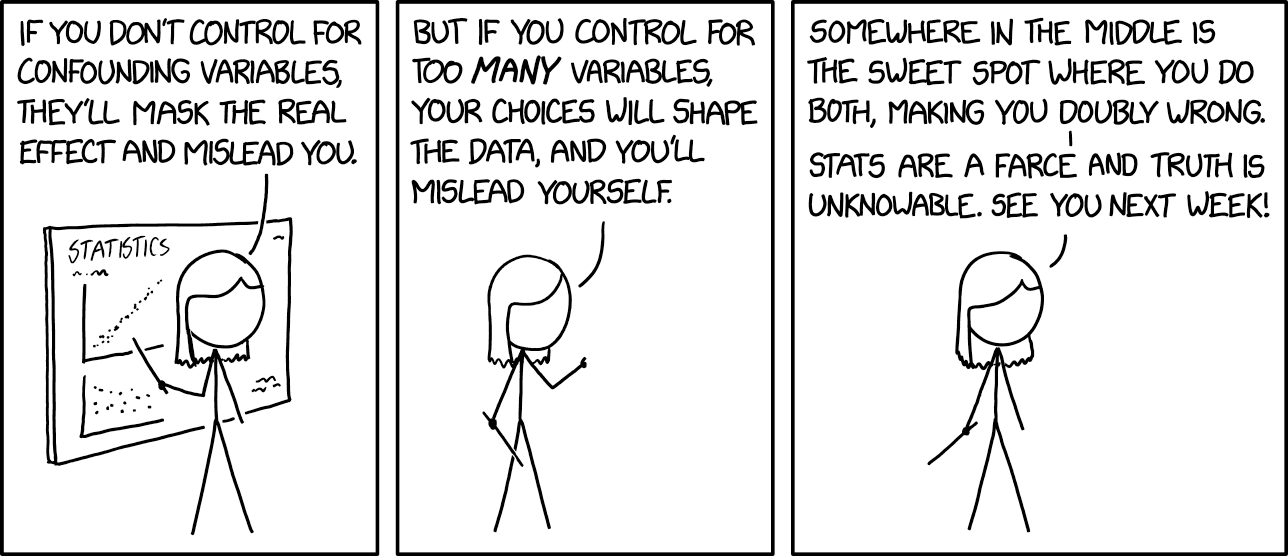
\includegraphics{images/confounding_variables.png}
\end{center}

\setlength{\abovedisplayskip}{-5pt}
\setlength{\abovedisplayshortskip}{-5pt}

{
\hypersetup{linkcolor=}
\setcounter{tocdepth}{2}
\tableofcontents
}
\listoffigures
\listoftables
\hypertarget{prefazione}{%
\chapter*{Prefazione}\label{prefazione}}


\emph{Data Science per psicologi} contiene il materiale delle lezioni dell'insegnamento di \emph{Psicometria B000286} (A.A. 2021/2022) rivolto agli studenti del primo anno del Corso di Laurea in Scienze e Tecniche Psicologiche dell'Università degli Studi di Firenze. \emph{Psicometria} si propone di fornire agli studenti un'introduzione all'analisi dei dati in psicologia. Le conoscenze/competenze che verranno sviluppate in questo insegnamento sono quelle della Data science, ovvero un insieme di conoscenze/competenze che si pongono all'intersezione tra statistica (ovvero, richiedono la capacità di comprendere teoremi statistici) e informatica (ovvero, richiedono la capacità di sapere utilizzare un software).

\hypertarget{la-psicologia-e-la-data-science}{%
\section*{La psicologia e la Data science}\label{la-psicologia-e-la-data-science}}


Sembra sensato spendere due parole su un tema che è importante per gli studenti: quello indicato dal titolo di questo Capitolo. È ovvio che agli studenti di psicologia la statistica non piace. Se piacesse, forse studierebbero Data science e non psicologia; ma non lo fanno. Di conseguenza, gli studenti di psicologia si chiedono: ``perché dobbiamo perdere tanto tempo a studiare queste cose quando in realtà quello che ci interessa è tutt'altro?'' Questa è una bella domanda.

C'è una ragione molto semplice che dovrebbe farci capire perché la Data science è così importante per la psicologia. Infatti, a ben pensarci, la psicologia è una disciplina intrinsecamente statistica, se per statistica intendiamo quella disciplina che studia la variazione delle caratteristiche degli individui nella popolazione. La psicologia studia \emph{gli individui} ed è proprio la variabilità inter- e intra-individuale ciò che vogliamo descrivere e, in certi casi, predire. In questo senso, la psicologia è molto diversa dall'ingegneria, per esempio. Le proprietà di un determinato ponte sotto certe condizioni, ad esempio, sono molto simili a quelle di un altro ponte, sotto le medesime condizioni. Quindi, per un ingegnere la statistica è poco importante: le proprietà dei materiali sono unicamente dipendenti dalla loro composizione e restano costanti. Ma lo stesso non può dirsi degli individui: ogni individuo è unico e cambia nel tempo. E le variazioni tra gli individui, e di un individuo nel tempo, sono l'oggetto di studio proprio della psicologia: è dunque chiaro che i problemi che la psicologia si pone sono molto diversi da quelli affrontati, per esempio, dagli ingegneri. Questa è la ragione per cui abbiamo tanto bisogno della Data science in psicologia: perché la Data science ci consente di descrivere la variazione e il cambiamento. E queste sono appunto le caratteristiche di base dei fenomeni psicologici.

Sono sicuro che, leggendo queste righe, a molti studenti sarà venuta in mente la seguente domanda: perché non chiediamo a qualche esperto di fare il ``lavoro sporco'' (ovvero le analisi statistiche) per noi, mentre noi (gli psicologi) ci occupiamo solo di ciò che ci interessa, ovvero dei problemi psicologici slegati dai dettagli ``tecnici'' della Data science? La risposta a questa domanda è che non è possibile progettare uno studio psicologico sensato senza avere almeno una comprensione rudimentale della Data science. Le tematiche della Data science non possono essere ignorate né dai ricercatori in psicologia né da coloro che svolgono la professione di psicologo al di fuori dell'Università. Infatti, anche i professionisti al di fuori dall'università non possono fare a meno di leggere la letteratura psicologica più recente: il continuo aggiornamento delle conoscenze è infatti richiesto dalla deontologia della professione. Ma per potere fare questo è necessario conoscere un bel po' di Data science! Basta aprire a caso una rivista specialistica di psicologia per rendersi conto di quanto ciò sia vero: gli articoli che riportano i risultati delle ricerche psicologiche sono zeppi di analisi statistiche e di modelli formali. E la comprensione della letteratura psicologica rappresenta un requisito minimo nel bagaglio professionale dello psicologo.

Le considerazioni precedenti cercano di chiarire il seguente punto: la Data science non è qualcosa da studiare a malincuore, in un singolo insegnamento universitario, per poi poterla tranquillamente dimenticare. Nel bene e nel male, gli psicologi usano gli strumenti della Data science in tantissimi ambiti della loro attività professionale: in particolare quando costruiscono, somministrano e interpretano i test psicometrici. È dunque chiaro che possedere delle solide basi di Data science è un tassello imprescindibile del bagaglio professionale dello psicologo. In questo insegnamento verrano trattati i temi base della Data science e verrà adottato un punto di vista bayesiano, che corrisponde all'approccio più recente e sempre più diffuso in psicologia.

\hypertarget{come-studiare}{%
\section*{Come studiare}\label{come-studiare}}


Il giusto metodo di studio per prepararsi all'esame di Psicometria è quello di seguire attivamente le lezioni, assimilare i concetti via via che essi vengono presentati e verificare in autonomia le procedure presentate a lezione. Incoraggio gli studenti a farmi domande per chiarire ciò che non è stato capito appieno. Incoraggio gli studenti a utilizzare i forum attivi su Moodle e, soprattutto, a svolgere gli esercizi proposti su Moodle. I problemi forniti su Moodle rappresentano il livello di difficoltà richiesto per superare l'esame e consentono allo studente di comprendere se le competenze sviluppate fino a quel punto sono sufficienti rispetto alle richieste dell'esame.

La prima fase dello studio, che è sicuramente individuale, è quella in cui è necessario acquisire le conoscenze teoriche relative ai problemi che saranno presentati all'esame. La seconda fase di studio, che può essere facilitata da scambi con altri e da incontri di gruppo, porta ad acquisire la capacità di applicare le conoscenze: è necessario capire come usare un software (\(\textsf{R}\)) per applicare i concetti statistici alla specifica situazione del problema che si vuole risolvere. Le due fasi non sono però separate: il saper fare molto spesso ci aiuta a capire meglio.

\hypertarget{sviluppare-un-metodo-di-studio-efficace}{%
\section*{Sviluppare un metodo di studio efficace}\label{sviluppare-un-metodo-di-studio-efficace}}


Avendo insegnato molte volte in passato un corso introduttivo di analisi dei dati ho notato nel corso degli anni che gli studenti con l'atteggiamento mentale che descriverò qui sotto generalmente ottengono ottimi risultati. Alcuni studenti sviluppano naturalmente questo approccio allo studio, ma altri hanno bisogno di fare uno sforzo per maturarlo. Fornisco qui sotto una breve descrizione del ``metodo di studio'' che, nella mia esperienza, è il più efficace per affrontare le richieste di questo insegnamento.

\begin{itemize}
\tightlist
\item
  Dedicate un tempo sufficiente al materiale di base, apparentemente facile; assicuratevi di averlo capito bene. Cercate le lacune nella vostra comprensione. Leggere presentazioni diverse dello stesso materiale (in libri o articoli diversi) può fornire nuove intuizioni.
\item
  Gli errori che facciamo sono i nostri migliori maestri. Istintivamente cerchiamo di dimenticare subito i nostri errori. Ma il miglior modo di imparare è apprendere dagli errori che commettiamo. In questo senso, una soluzione corretta è meno utile di una soluzione sbagliata. Quando commettiamo un errore questo ci fornisce un'informazione importante: ci fa capire qual è il materiale di studio sul quale dobbiamo ritornare e che dobbiamo capire meglio.
\item
  C'è ovviamente un aspetto ``psicologico'' nello studio. Quando un esercizio o problema ci sembra incomprensibile, la cosa migliore da fare è dire: ``mi arrendo'', ``non ho idea di cosa fare!''. Questo ci rilassa: ci siamo già arresi, quindi non abbiamo niente da perdere, non dobbiamo più preoccuparci. Ma non dobbiamo fermarci qui. Le cose ``migliori'' che faccio (se ci sono) le faccio quando non ho voglia di lavorare. Alle volte, quando c'è qualcosa che non so fare e non ho idea di come affontare, mi dico: ``oggi non ho proprio voglia di fare fatica'', non ho voglia di mettermi nello stato mentale per cui ``in 10 minuti devo risolvere il problema perché dopo devo fare altre cose''. Però ho voglia di \emph{divertirmi} con quel problema e allora mi dedico a qualche aspetto ``marginale'' del problema, che so come affrontare, oppure considero l'aspetto più difficile del problema, quello che non so come risolvere, ma invece di cercare di risolverlo, guardo come altre persone hanno affrontato problemi simili, opppure lo stesso problema in un altro contesto. Non mi pongo l'obiettivo ``risolvi il problema in 10 minuti'', ma invece quello di farmi un'idea ``generale'' del problema, o quello di capire un caso più specifico e più semplice del problema. Senza nessuna pressione. Infatti, in quel momento ho deciso di non lavorare (ovvero, di non fare fatica). Va benissimo se ``parto per la tangente'', ovvero se mi metto a leggere del materiale che sembra avere poco a che fare con il problema centrale (le nostre intuizioni e la nostra curiosità solitamente ci indirizzano sulla strada giusta). Quando faccio così, molto spesso trovo la soluzione del problema che mi ero posto e, paradossalmente, la trovo in un tempo minore di quello che, in precedenza, avevo dedicato a ``lavorare'' al problema. Allora perché non faccio sempre così? C'è ovviamente l'aspetto dei ``10 minuti'' che non è sempre facile da dimenticare. Sotto pressione, possiamo solo agire in maniera automatica, ovvero possiamo solo applicare qualcosa che già sappiamo fare. Ma se dobbiamo imparare qualcosa di nuovo, la pressione è un impedimento.
\item
  È utile farsi da soli delle domande sugli argomenti trattati, senza limitarsi a cercare di risolvere gli esercizi che vengono assegnati. Quando studio qualcosa mi viene in mente: ``se questo è vero, allora deve succedere quest'altra cosa''. Allora verifico se questo è vero, di solito con una simulazione. Se i risultati della simulazione sono quelli che mi aspetto, allora vuol dire che ho capito. Se i risultati sono diversi da quelli che mi aspettavo, allora mi rendo conto di non avere capito e ritorno indietro a studiare con più attenzione la teoria che pensavo di avere capito -- e ovviamente mi rendo conto che c'era un aspetto che avevo frainteso. Questo tipo di verifica è qualcosa che dobbiamo fare da soli, in prima persona: nessun altro può fare questo al posto nostro.
\item
  Non aspettatevi di capire tutto la prima volta che incontrate un argomento nuovo.\footnote{Ricordatevi inoltre che gli individui tendono a sottostimare la propria capacità di apprendere \citep{horn2021underestimating}.} È utile farsi una nota mentalmente delle lacune nella vostra comprensione e tornare su di esse in seguito per carcare di colmarle. L'atteggiamento naturale, quando non capiamo i dettagli di qualcosa, è quello di pensare: ``non importa, ho capito in maniera approssimativa questo punto, non devo preoccuparmi del resto''. Ma in realtà non è vero: se la nostra comprensione è superficiale, quando il problema verrà presentato in una nuova forma, non riusciremo a risolverlo. Per cui i dubbi che ci vengono quando studiamo qualcosa sono il nostro alleato più prezioso: ci dicono esattamente quali sono gli aspetti che dobbiamo approfondire per potere migliorare la nostra preparazione.
\item
  È utile sviluppare una visione d'insieme degli argomenti trattati, capire l'obiettivo generale che si vuole raggiungere e avere chiaro il contributo che i vari pezzi di informazione forniscono al raggiungimento di tale obiettivo. Questa organizzazione mentale del materiale di studio facilita la comprensione. È estremamente utile creare degli schemi di ciò che si sta studiando. Non aspettate che sia io a fornirvi un riepilogo di ciò che dovete imparare: sviluppate da soli tali schemi e tali riassunti.
\item
  Tutti noi dobbiamo imparare l'arte di trovare le informazioni, non solo nel caso di questo insegnamento. Quando vi trovate di fronte a qualcosa che non capite, o ottenete un oscuro messaggio di errore da un software, ricordatevi: ``Google is your friend''!
\end{itemize}

\begin{flushright}
Corrado Caudek\\
Marzo 2022 \end{flushright}

\mainmatter

\hypertarget{part-inferenza-bayesiana}{%
\part{Inferenza bayesiana}\label{part-inferenza-bayesiana}}

\hypertarget{ch:intro-bayes-inference}{%
\chapter{Flusso di lavoro bayesiano}\label{ch:intro-bayes-inference}}

La moderna statistica bayesiana viene per lo più eseguita utilizzando un linguaggio di programmazione probabilistico implementato su computer. Ciò ha cambiato radicalmente il modo in cui venivano eseguite le statistiche bayesiane anche fin pochi decenni fa. La complessità dei modelli che possiamo costruire è aumentata e la barriera delle competenze matematiche e computazionali che sono richieste è diminuita. Inoltre, il processo di modellazione iterativa è diventato, sotto molti aspetti, molto più facile da eseguire. Anche se formulare modelli statistici complessi è diventato più facile che mai, la statistica è un campo pieno di sottigliezze che non scompaiono magicamente utilizzando potenti metodi computazionali. Pertanto, avere una buona preparazione sugli aspetti teorici, specialmente quelli rilevanti nella pratica, è estremamente utile per applicare efficacemente i metodi statistici.

\hypertarget{modellizzazione-bayesiana}{%
\section{Modellizzazione bayesiana}\label{modellizzazione-bayesiana}}

L'analisi bayesiana corrisponde alla costruzione di un modello statistico che si può rappresentare con una quaterna

\begin{equation}
(\mathcal{Y}, p(y \mid \theta), p(\theta), \theta \in \Theta),
\end{equation}

dove \(\mathcal{Y}\) è l'insieme di tutti i possibili risultati ottenuti dall'esperimento casuale e \(p(y \mid \theta)\) è una famiglia di leggi di probabilità, indicizzata dal parametro \(\theta \in \Theta\), che descrive l'incertezza sull'esito dell'esperimento. Secondo l'approccio bayesiano, il parametro incognito \(\theta\) è considerato una variabile casuale che segue la legge di probabilità \(p(\theta)\). L'incertezza su \(\theta\) è la sintesi delle opinioni e delle informazioni che si hanno sul parametro prima di avere osservato il risultato dell'esperimento e prende il nome di \emph{distribuzione a priori}. La costruzione del modello statistico passa attraverso la scelta di una densità \(p(y \mid \theta)\) che rappresenta, in senso probabilistico, il fenomeno d'interesse, e attraverso la scelta di una distribuzione a priori \(p(\theta)\). Le informazioni che si hanno a priori sul parametro di interesse \(\theta\), contenute in \(p(\theta)\), vengono aggiornate attraverso quelle provenienti dal campione osservato \(y = (y_1, \dots, y_n)\) contenute nella funzione \(p(y \mid \theta)\), che, osservata come funzione di \(\theta\) per \(y\), prende il nome di \emph{funzione di verosimiglianza}. L'aggiornamento delle informazioni avviene attraverso la formula di Bayes

\begin{equation}
p(\theta \mid y) = \frac{p(y \mid \theta) p(\theta)}{\int_{\Theta}p(y \mid \theta) p(\theta) \,\operatorname {d}\!\theta} \quad \theta \in \Theta,
 \label{eq:bayes-intro}
\end{equation}

in cui \(p(\theta \mid y)\) prende il nome di \emph{distribuzione a posteriori}.

Il denominatore del Teorema di Bayes \eqref{eq:bayes-intro}, che costituisce la costante di normalizzazione, è la densità marginale dei dati (o verosimiglianza marginale). In ambito bayesiano la distribuzione a posteriori viene utilizzata per calcolare le principali quantità di interesse dell'inferenza, ad esempio la media a posteriori di \(\theta\).

Possiamo descrivere la modellazione bayesiana distinguendo tre passaggi \citep{martin2022bayesian}.

\begin{enumerate}
\def\labelenumi{\arabic{enumi}.}
\tightlist
\item
  Dati alcuni dati e alcune ipotesi su come questi dati potrebbero essere stati generati, progettiamo un modello combinando e trasformando variabili casuali.
\item
  Usiamo il teorema di Bayes per condizionare i nostri modelli ai dati disponibili. Chiamiamo questo processo ``inferenza'' e come risultato otteniamo una distribuzione a posteriori.
\item
  Critichiamo il modello verificando se il modello abbia senso utilizzando criteri diversi, inclusi i dati e la nostra conoscenza del dominio. Poiché generalmente siamo incerti sui modelli, a volte confrontiamo modelli diversi.
\end{enumerate}

Questi tre passaggi vengono eseguiti in modo iterativo e danno luogo a quello che è chiamato ``flusso di lavoro bayesiano'' (\emph{bayesian workflow}).

\hypertarget{notazione}{%
\subsection{Notazione}\label{notazione}}

Per fissare la notazione, nel seguito \(y\) rappresenterà i dati e \(\theta\) rappresenterà i parametri incogniti di un modello statistico. Sia \(y\) che \(\theta\) vengono concepiti come variabili casuali. Con \(x\) vengono invece denotate le quantità note, come ad esempio i predittori del modello lineare. Per rappresentare in un modo conciso i modelli probabilistici viene usata una notazione particolare. Ad esempio, invece di scrivere \(p(\theta) = \mbox{Beta}(1, 1)\) scriviamo \(\theta \sim \mbox{Beta}(1, 1)\). Il simbolo ``\(\sim\)'' viene spesso letto ``è distribuito come''. Possiamo anche pensare che significhi che \(\theta\) costituisce un campione casuale estratto dalla distribuzione Beta(1, 1). Allo stesso modo, ad esempio, la verosimiglianza del modello binomiale può essere scritta come \(y \sim \text{Bin}(n, \theta)\).

\hypertarget{distribuzioni-a-priori}{%
\section{Distribuzioni a priori}\label{distribuzioni-a-priori}}

Quando adottiamo un approccio bayesiano, i parametri della distribuzione di riferimento non venono considerati come delle costanti incognite ma bensì vengono trattati come variabili casuali; di conseguenza, i parametri assumono una particolare distribuzione che nelle statistica bayesiana viene definita ``a priori''. I parametri (o il parametro), che possiamo indicare con \(\theta\), possono assumere delle distribuzioni a priori differenti: a seconda delle informazioni disponibili bisogna selezionare una distribuzione di \(\theta\) in modo tale che venga assegnata una probabilità maggiore a quei valori che si ritengono più plausibili per \(\theta\). Idealmente, le credenze a priori che portano alla specificazione di una distribuzione a priori dovrebbero essere supportate da una qualche motivazione, come ad esempio i risultati di ricerche precedenti.

\hypertarget{tipologie-di-distribuzioni-a-priori}{%
\subsection{Tipologie di distribuzioni a priori}\label{tipologie-di-distribuzioni-a-priori}}

Possiamo distinguere tra diverse distribuzioni a priori in base a quanto fortemente impegnano il ricercatore a ritenere come plausibile un particolare intervallo di valori dei parametri. Il caso più estremo è quello che rivela una totale assenza di conoscenze a priori, il che conduce alle \emph{distribuzioni a priori non informative}, ovvero quelle che assegnano lo stesso livello di credibilità a tutti i valori dei parametri. Le distribuzioni a priori informative, d'altra parte, possono essere \emph{debolmente informative} o \emph{fortemente informative}, a seconda della forza della credenza che esprimono. Il caso più estremo di credenza a priori è quello che riassume il punto di vista del ricercatore nei termini di un \emph{unico valore} del parametro, il che assegna tutta la probabilità (massa o densità) ad di un singolo valore del parametro. Poiché questa non è più una distribuzione di probabilità, sebbene ne soddisfi la definizione, in questo caso si parla di una \emph{distribuzione a priori degenerata}. La figura seguente motra alcuni esempi di distribuzioni a priori per il modello Binomiale:

\begin{itemize}
\tightlist
\item
  distribuzione \emph{non informativa}: \(\theta_c \sim \mbox{Beta}(1,1)\);
\item
  distribuzione \emph{debolmente informativa}: \(\theta_c \sim \mbox{Beta}(5,2)\);
\item
  distribuzione \emph{fortemente informativa}: \(\theta_c \sim \mbox{Beta}(50,20)\);
\item
  \emph{valore puntuale}: \(\theta_c \sim \mbox{Beta}(\alpha, \beta)\) con \(\alpha, \beta \rightarrow \infty\) e \(\frac{\alpha}{\beta} = \frac{5}{2}\).
\end{itemize}

\begin{figure}[h]

{\centering 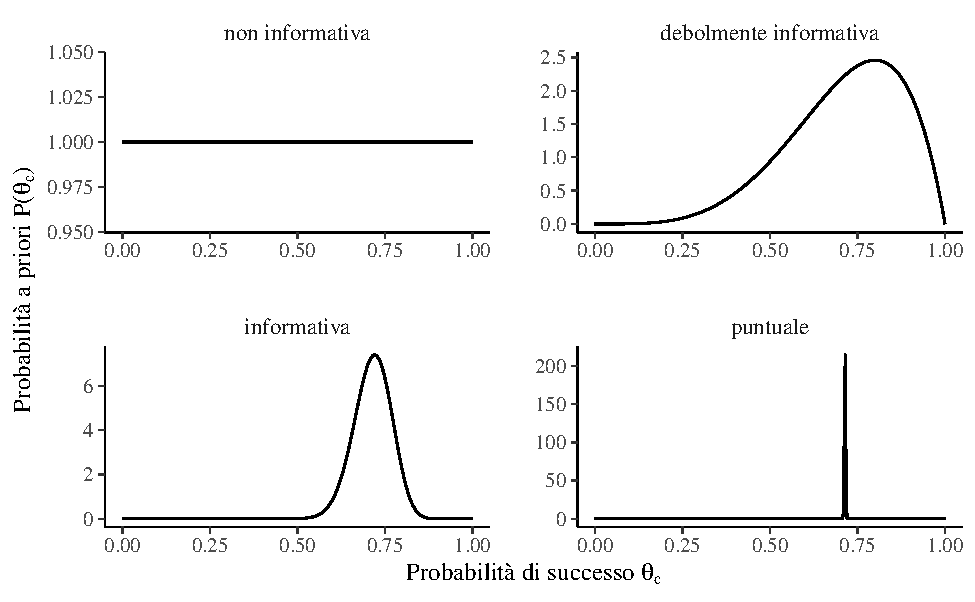
\includegraphics{ds4psy_files/figure-latex/unnamed-chunk-3-1} 

}

\caption{Esempi di distribuzioni a priori per il parametro $\theta_c$ nel Modello Binomiale.}\label{fig:unnamed-chunk-3}
\end{figure}

\hypertarget{selezione-della-distribuzione-a-priori}{%
\subsection{Selezione della distribuzione a priori}\label{selezione-della-distribuzione-a-priori}}

La selezione delle distribuzioni a priori è stata spesso vista come una delle scelte più importanti che un ricercatore fa quando implementa un modello bayesiano in quanto può avere un impatto sostanziale sui risultati finali. La soggettività delle distribuzioni a priori è evidenziata dai critici come un potenziale svantaggio dei metodi bayesiani. A questa critica, \citet{vandeSchoot2021modelling} rispondono dicendo che, al di là della scelta delle distribuzioni a priori, ci sono molti elementi del processo di inferenza statistica che sono soggettivi, ovvero la scelta del modello statistico e le ipotesi sulla distribuzione degli errori. In secondo luogo, \citet{vandeSchoot2021modelling} notano come le distribuzioni a priori svolgono due importanti ruoli statistici: quello della ``regolarizzazione della stima'', ovvero, il processo che porta ad indebolire l'influenza indebita di osservazioni estreme, e quello del miglioramento dell'efficienza della stima, ovvero, la facilitazione dei processi di calcolo numerico di stima della distribuzione a posteriori. L'effetto della distribuzione a priori sulla distribuzione a posteriori verrà discusso in dettaglio nel Capitolo \ref{chapter-balance}.

\hypertarget{un-esempio-concreto}{%
\subsection{Un esempio concreto}\label{un-esempio-concreto}}

Per introdurre la modelizzazione bayesiana useremo qui i dati riportati da \citet{zetschefuture2019} (si veda l'appendice \ref{appendix:future-exp}). Tali dati corrispondono a 23 ``successi'' in 30 prove e possono dunque essere considerati la manifestazione di una variabile casuale Bernoulliana.

Se non abbiamo alcuna informazione a priori su \(\theta\) (ovvero, la probabilità che l'aspettativa dell'umore futuro del partecipante sia distorta negativamente), potremmo pensare di usare una distribuzione a priori uniforme, ovvero una Beta di parametri \(\alpha=1\) e \(\beta=1\). Una tale scelta, tuttavia, è sconsigliata in quanto è più vantaggioso usare una distribuzione debolmente informativa, come ad esempio \(\mbox{Beta}(2, 2)\), che ha come scopo la regolarizzazione, cioè quello di mantenere le inferenze in un intervallo ragionevole. Qui useremo una \(\mbox{Beta}(2, 10)\).

\[
p(\theta) = \frac{\Gamma(12)}{\Gamma(2)\Gamma(10)}\theta^{2-1} (1-\theta)^{10-1}.
\]

\begin{Shaded}
\begin{Highlighting}[]
\NormalTok{bayesrules}\SpecialCharTok{::}\FunctionTok{plot\_beta}\NormalTok{(}\AttributeTok{alpha =} \DecValTok{2}\NormalTok{, }\AttributeTok{beta =} \DecValTok{10}\NormalTok{, }\AttributeTok{mean =} \ConstantTok{TRUE}\NormalTok{, }\AttributeTok{mode =} \ConstantTok{TRUE}\NormalTok{)}
\end{Highlighting}
\end{Shaded}

\begin{center}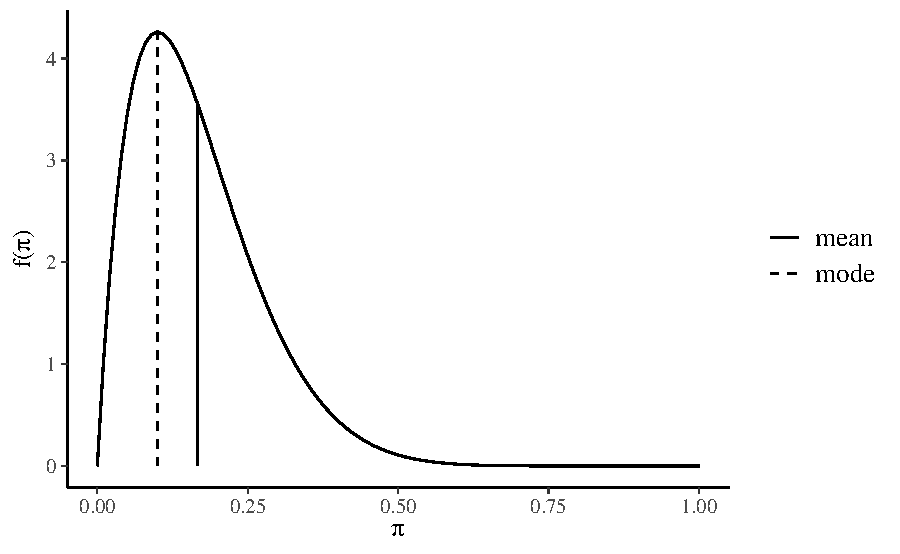
\includegraphics{ds4psy_files/figure-latex/unnamed-chunk-4-1} \end{center}

La \(\mbox{Beta}(2, 10)\) esprime la credenza che \(\theta\) assume valori \(< 0.5\), con il valore più plausibile pari a circa 0.1. Questo è assolutamente implausibile per il caso dell'esempio in discussione: la \(\mbox{Beta}(2, 10)\) verrà usata solo per scopi didattici, ovvero, per esplorare le conseguenze di tale scelta sulla distribuzione a posteriori.

\hypertarget{la-funzione-di-verosimiglianza}{%
\section{La funzione di verosimiglianza}\label{la-funzione-di-verosimiglianza}}

Iniziamo con una definizione.

\begin{definition}
La \emph{funzione di verosimiglianza} \(\mathcal{L}(\theta \mid y) = f(y \mid \theta), \theta \in \Theta,\) è la funzione di massa o di densità di probabilità dei dati \(y\) vista come una funzione del parametro sconosciuto (o dei parametri sconosciuti) \(\theta\).
\end{definition}

Detto in altre parole, le funzioni di verosimiglianza e di (massa o densità di) probabilità sono formalmente identiche, ma è completamente diversa la loro interpretazione. Nel caso della funzione di massa o di densità di probabilità la distribuzione del vettore casuale delle osservazioni campionarie \(y\) dipende dai valori assunti dal parametro (o dai parametri) \(\theta\); nel caso della la funzione di verosimiglianza la credibilità assegnata a ciascun possibile valore \(\theta\) viene determinata avendo acquisita l'informazione campionaria \(y\) che rappresenta l'elemento condizionante. In altri termini, la funzione di verosimiglianza descrive in termini relativi il sostegno empirico che \(\theta \in \Theta\) riceve da \(y\). Infatti, la funzione di verosimiglianza assume forme diverse al variare di \(y\). Possiamo dunque pensare alla funzione di verosimiglianza come alla risposta alla seguente domanda: avendo osservato i dati \(y\), quanto risultano (relativamente) credibili i diversi valori del parametro \(\theta\)? In termini più formali possiamo dire: sulla base dei dati, \(\theta_1 \in \Theta\) risulta più credibile di \(\theta_2 \in \Theta\) quale indice del modello probabilistico generatore dei dati se \(\mathcal{L}(\theta_1) > \mathcal{L}(\theta_1)\).

Notiamo un punto importante: la funzione \(\mathcal{L}(\theta \mid y)\) non è una funzione di densità. Infatti, essa non racchiude un'area unitaria.

\hypertarget{notazione-1}{%
\subsection{Notazione}\label{notazione-1}}

Seguendo una pratica comune, in questa dispensa spesso useremo la notazione \(p(\cdot)\) per rappresentare due quantità differenti, ovvero la funzione di verosimiglianza e la distribuzione a priori. Questo piccolo abuso di notazione riflette il seguente punto di vista: anche se la verosimiglianza non è una funzione di densità di probabilità, noi non vogliamo stressare questo aspetto, ma vogliamo piuttosto pensare alla verosimiglianza e alla distribuzione a priori come a due elementi che sono egualmente necessari per calcolare la distribuzione a posteriori. In altri termini, per così dire, questa notazione assegna lo stesso status epistemologico alle due diverse quantità che si trovano al numeratore della regola di Bayes.

\hypertarget{la-log-verosimiglianza}{%
\subsection{La log-verosimiglianza}\label{la-log-verosimiglianza}}

Dal punto di vista pratico risulta più conveniente utilizzare, al posto della funzione di verosimiglianza, il suo logaritmo naturale, ovvero la funzione di log-verosimiglianza:

\begin{equation}
\ell(\theta) = \log \mathcal{L}(\theta).
\end{equation}

Poiché il logaritmo è una funzione strettamente crescente (usualmente si considera il logaritmo naturale), allora \(\mathcal{L}(\theta)\) e \(\ell(\theta)\) assumono il massimo (o i punti di massimo) in corrispondenza degli stessi valori di \(\theta\) (per un approfondimento, si veda l'Appendice \ref{appendix:max-like}):

\[
\hat{\theta} = \argmax_{\theta \in \Theta} \ell(\theta) = \argmax_{\theta \in \Theta} \mathcal{L}(\theta).
\]

Per le proprietà del logaritmo, si ha

\begin{equation}
\ell(\theta) = \log \left( \prod_{i = 1}^n f(y \mid \theta) \right) = \sum_{i = 1}^n \log f(y \mid \theta).
\end{equation}

Si noti che non è necessario lavorare con i logaritmi, ma è fortemente consigliato. Il motivo è che i valori della verosimiglianza, in cui si moltiplicano valori di probabilità molto piccoli, possono diventare estremamente piccoli -- qualcosa come \(10^{-34}\). In tali circostanze, non è sorprendente che i programmi dei computer mostrino problemi di arrotondamento numerico. Le trasformazioni logaritmiche risolvono questo problema.

\hypertarget{un-esempio-concreto-1}{%
\subsection{Un esempio concreto}\label{un-esempio-concreto-1}}

Se i dati di \citet{zetschefuture2019} possono essere riassunti da una proporzione allora è sensato adottare un modello probabilistico binomiale quale meccanismo generatore dei dati:

\begin{equation}
y  \sim \mbox{Bin}(n, \theta),
\label{eq:binomialmodel}
\end{equation}

laddove \(\theta\) è la probabiltà che una prova Bernoulliana assuma il valore 1 e \(n\) corrisponde al numero di prove Bernoulliane. Questo modello assume che le prove Bernoulliane \(y_i\) che costituiscono il campione \(y\) siano tra loro indipendenti e che ciascuna abbia la stessa probabilità \(\theta \in [0, 1]\) di essere un ``successo'' (valore 1). In altre parole, il modello generatore dei dati avrà una funzione di massa di probabilità

\[
p(y \mid \theta)
\ = \
\mbox{Bin}(y \mid n, \theta).
\]

Nei capitoli precedenti è stato mostrato come, sulla base del modello binomiale, sia possibile assegnare una probabilità a ciascun possibile valore \(y \in \{0, 1, \dots, n\}\) \emph{assumendo noto il valore del parametro} \(\theta\). Ma ora abbiamo il problema inverso, ovvero quello di fare inferenza su \(\theta\) alla luce dei dati campionari \(y\). In altre parole, riteniamo di conoscere il modello probabilistico che ha generato i dati, ma di tale modello non conosciamo i parametri: vogliamo dunque ottenere informazioni su \(\theta\) avendo osservato i dati \(y\).

Per i dati di \citet{zetschefuture2019} la funzione di verosimiglianza corrisponde alla funzione binomiale di parametro \(\theta \in [0, 1]\) sconosciuto. Abbiamo osservato un ``successo'' 23 volte in 30 ``prove'', dunque, \(y = 23\) e \(n = 30\). La funzione di verosimiglianza diventa

\begin{equation}
\mathcal{L}(\theta \mid y) = \frac{(23 + 7)!}{23!7!} \theta^{23} + (1-\theta)^7.
\label{eq:likebino23}
\end{equation}

Per costruire la funzione di verosimiglianza dobbiamo applicare la \eqref{eq:likebino23} tante volte, cambiando ogni volta il valore \(\theta\) ma \emph{tenendo sempre costante il valore dei dati}. Per esempio, se poniamo \(\theta = 0.1\)

\[
\mathcal{L}(\theta \mid y) = \frac{(23 + 7)!}{23!7!} 0.1^{23} + (1-0.1)^7
\]

otteniamo

\begin{Shaded}
\begin{Highlighting}[]
\FunctionTok{dbinom}\NormalTok{(}\DecValTok{23}\NormalTok{, }\DecValTok{30}\NormalTok{, }\FloatTok{0.1}\NormalTok{)}
\CommentTok{\#\textgreater{} [1] 9.737e{-}18}
\end{Highlighting}
\end{Shaded}

Se poniamo \(\theta = 0.2\)

\[
\mathcal{L}(\theta \mid y) = \frac{(23 + 7)!}{23!7!} 0.2^{23} + (1-0.2)^7
\]

otteniamo

\begin{Shaded}
\begin{Highlighting}[]
\FunctionTok{dbinom}\NormalTok{(}\DecValTok{23}\NormalTok{, }\DecValTok{30}\NormalTok{, }\FloatTok{0.2}\NormalTok{)}
\CommentTok{\#\textgreater{} [1] 3.581e{-}11}
\end{Highlighting}
\end{Shaded}

e così via. La figura \ref{fig:likefutexpect} --- costruita utilizzando 100 valori equispaziati \(\theta \in [0, 1]\) --- fornisce una rappresentazione grafica della funzione di verosimiglianza.

\begin{Shaded}
\begin{Highlighting}[]
\NormalTok{n }\OtherTok{\textless{}{-}} \DecValTok{30}
\NormalTok{y }\OtherTok{\textless{}{-}} \DecValTok{23}
\NormalTok{theta }\OtherTok{\textless{}{-}} \FunctionTok{seq}\NormalTok{(}\DecValTok{0}\NormalTok{, }\DecValTok{1}\NormalTok{, }\AttributeTok{length.out =} \DecValTok{100}\NormalTok{)}
\NormalTok{like }\OtherTok{\textless{}{-}} \FunctionTok{choose}\NormalTok{(n, y) }\SpecialCharTok{*}\NormalTok{ theta}\SpecialCharTok{\^{}}\NormalTok{y }\SpecialCharTok{*}\NormalTok{ (}\DecValTok{1} \SpecialCharTok{{-}}\NormalTok{ theta)}\SpecialCharTok{\^{}}\NormalTok{(n }\SpecialCharTok{{-}}\NormalTok{ y)}
\FunctionTok{tibble}\NormalTok{(theta, like) }\SpecialCharTok{\%\textgreater{}\%}
  \FunctionTok{ggplot}\NormalTok{(}\FunctionTok{aes}\NormalTok{(}\AttributeTok{x =}\NormalTok{ theta, }\AttributeTok{y =}\NormalTok{ like)) }\SpecialCharTok{+}
  \FunctionTok{geom\_line}\NormalTok{() }\SpecialCharTok{+}
  \FunctionTok{labs}\NormalTok{(}
    \AttributeTok{y =} \FunctionTok{expression}\NormalTok{(}\FunctionTok{L}\NormalTok{(theta)),}
    \AttributeTok{x =} \FunctionTok{expression}\NormalTok{(}\StringTok{"Valori possibili di"} \SpecialCharTok{\textasciitilde{}}\NormalTok{ theta)}
\NormalTok{  )}
\end{Highlighting}
\end{Shaded}

\begin{figure}[h]

{\centering 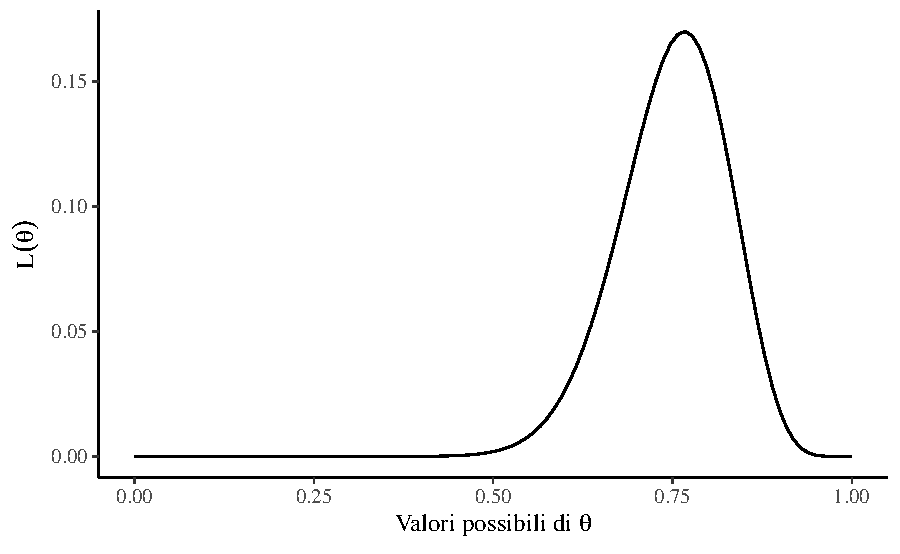
\includegraphics{ds4psy_files/figure-latex/likefutexpect-1} 

}

\caption{Funzione di verosimiglianza nel caso di 23 successi in 30 prove.}\label{fig:likefutexpect}
\end{figure}

Come possiamo interpretare la curva che abbiamo ottenuto? Per alcuni valori \(\theta\) la funzione di verosimiglianza assume valori piccoli; per altri valori \(\theta\) la funzione di verosimiglianza assume valori più grandi. Questi ultimi sono i valori di \(\theta\) più credibili e il valore 23/30 (la moda della funzione di verosimiglianza) è il valore più credibile di tutti.

\hypertarget{sec:const-normaliz-bino23}{%
\section{La verosimiglianza marginale}\label{sec:const-normaliz-bino23}}

Per il calcolo di \(p(\theta \mid y)\) è necessario dividere il prodotto tra la distribuzione a priori e la verosimiglianza per una costante di normalizzazione. Tale costante di normalizzazione, detta \emph{verosimiglianza marginale}, ha lo scopo di fare in modo che \(p(\theta \mid y)\) abbia area unitaria.

Si noti che, nel caso di variabili continue, la verosimiglianza marginale è espressa nei termini di un integrale. Tranne in pochi casi particolari, tale integrale non ha una soluzione analitica. Per questa ragione, l'inferenza bayesiana procede calcolando una approssimazione della distribuzione a posteriori mediante metodi numerici.

\hypertarget{un-esempio-concreto-2}{%
\subsection{Un esempio concreto}\label{un-esempio-concreto-2}}

Consideriamo nuovamente i dati di \citet{zetschefuture2019}. Supponiamo che nel numeratore bayesiano la verosimiglianza sia moltiplicata per una distribuzione uniforme, ovvero \(\mbox{Beta}(1, 1)\). In tali circostanze, il prodotto si riduce alla funzione di verosimiglianza. Per i dati di \citet{zetschefuture2019}, dunque, la costante di normalizzazione si ottiene marginalizzando la funzione di verosimiglianza \(p(y = 23, n = 30 \mid \theta)\) sopra \(\theta\), ovvero risolvendo l'integrale:

\begin{equation}
p(y = 23, n = 30) = \int_0^1 \binom{30}{23} \theta^{23} (1-\theta)^{7} \,\operatorname {d}\!\theta.
\label{eq:intlikebino23}
\end{equation}

Una soluzione numerica si trova facilmente usando \(\R\):

\begin{Shaded}
\begin{Highlighting}[]
\NormalTok{like\_bin }\OtherTok{\textless{}{-}} \ControlFlowTok{function}\NormalTok{(theta) \{}
  \FunctionTok{choose}\NormalTok{(}\DecValTok{30}\NormalTok{, }\DecValTok{23}\NormalTok{) }\SpecialCharTok{*}\NormalTok{ theta}\SpecialCharTok{\^{}}\DecValTok{23} \SpecialCharTok{*}\NormalTok{ (}\DecValTok{1} \SpecialCharTok{{-}}\NormalTok{ theta)}\SpecialCharTok{\^{}}\DecValTok{7}
\NormalTok{\}}
\FunctionTok{integrate}\NormalTok{(like\_bin, }\AttributeTok{lower =} \DecValTok{0}\NormalTok{, }\AttributeTok{upper =} \DecValTok{1}\NormalTok{)}\SpecialCharTok{$}\NormalTok{value}
\CommentTok{\#\textgreater{} [1] 0.03226}
\end{Highlighting}
\end{Shaded}

La derivazione analitica è fornita nell'Appendice \ref{appendix:const-norm-bino23}.

\hypertarget{distribuzione-a-posteriori}{%
\section{Distribuzione a posteriori}\label{distribuzione-a-posteriori}}

La distribuzione a postreriori si trova applicando il teorema di Bayes:

\[
\text{probabilità a posteriori} = \frac{\text{probabilità a priori} \cdot \text{verosimiglianza}}{\text{costante di normalizzazione}}
\]

Una volta trovata la distribuzione a posteriori, possiamo usarla per derivare altre quantità di interesse. Questo viene generalmente ottenuto calcolando il valore atteso:

\[
J = \int f(\theta) p(\theta \mid y) \,\operatorname {d}\!y
\]

Se \(f(\cdot)\) è la funzione identità, ad esempio, \(J\) risulta essere la media di \(\theta\):

\[
\bar{\theta} = \int_{\Theta} \theta p(\theta \mid y) \,\operatorname {d}\!\theta .
\]

Ripeto qui quanto detto sopra: le quantità di interesse della statistica bayesiana(costante di normalizzazione, valore atteso della distribuzione a posteriori, ecc.) contengono integrali che risultano, nella maggior parte dei casi, impossibili da risolvere analiticamente. Per questo motivo, si ricorre a metodi di stima numerici, in particolare a quei metodi Monte Carlo basati sulle proprietà delle catene di Markov (MCMC). Questo argomento verrà discusso nel Capitolo \ref{ch:metropolis}.

\hypertarget{distribuzione-predittiva-a-priori}{%
\section{Distribuzione predittiva a priori}\label{distribuzione-predittiva-a-priori}}

La distribuzione a posteriori è l'oggetto centrale nella statistica bayesiana, ma non è l'unico. Oltre a fare inferenze sui valori dei parametri, potremmo voler fare inferenze sui dati. Questo può essere fatto calcolando la \emph{distribuzione predittiva a priori}:

\begin{equation}
p(y^*) = \int_\Theta p(y^* \mid \theta) p(\theta) \,\operatorname {d}\!\theta .
\label{eq:prior-pred-distr}
\end{equation}

La \eqref{eq:prior-pred-distr} descrive la distribuzione prevista dei dati in base al modello (che include la distribuzione a priori e la verosimiglianza), ovvero descrive i dati \(y^*\) che ci aspettiamo di osservare, dato il modello, prima di avere osservato i dati del campione.

È possibile utilizzare campioni dalla distribuzione predittiva a priori per valutare e calibrare i modelli utilizzando le nostre conoscenze dominio-specifiche. Ad esempio, ci possiamo chiedere: ``È sensato che un modello dell'altezza umana preveda che un essere umano sia alto -1.5 metri?''. Già prima di misurare una singola persona, possiamo renderci conto dell'assurdità di questa domanda. Se la distribuzione prevista dei dati consente domande di questo tipo (ovvero, prevede di osservare dati che risultano insensati alla luce delle nostre conoscenze dominio-specifiche), è chiaro che il modello deve essere riformulato.

\hypertarget{distribuzione-predittiva-a-posteriori}{%
\section{Distribuzione predittiva a posteriori}\label{distribuzione-predittiva-a-posteriori}}

Un'altra quantità utile da calcolare è la distribuzione predittiva a posteriori:

\begin{equation}
p(\tilde{y} \mid y) = \int_\Theta p(\tilde{y} \mid \theta) p(\theta \mid y) \,\operatorname {d}\!\theta .
\label{eq:post-pred-distr}
\end{equation}

Questa è la distribuzione dei dati attesi futuri \(\tilde{y}\) alla luce della distribuzione a posteriori \(p(\theta \mid y)\), che a sua volta è una conseguenza del modello adottato (distribuzione a priori e verosimiglianza) e dei dati osservati. In altre parole, questi sono i dati che il modello si aspetta dopo aver osservato i dati de campione. Dalla \eqref{eq:post-pred-distr} possiamo vedere che le previsioni sui dati attesi futuri sono calcolate integrando (o marginalizzando) sulla distribuzione a posteriori dei parametri. Di conseguenza, le previsioni calcolate in questo modo incorporano l'incertezza relativa alla stima dei parametri del modello.

\hypertarget{commenti-e-considerazioni-finali}{%
\section*{Commenti e considerazioni finali}\label{commenti-e-considerazioni-finali}}


Questo Capitolo ha brevemente passato in rassegna i concetti di base dell'inferenza statistica bayesiana. In base all'approccio bayesiano, invece di dire che il parametro di interesse di un modello statistico ha un valore vero ma sconosciuto, diciamo che, prima di eseguire l'esperimento, è possibile assegnare una distribuzione di probabilità, che chiamano stato di credenza, a quello che è il vero valore del parametro. Questa distribuzione a priori può essere nota (per esempio, sappiamo che la distribuzione dei punteggi del QI è normale con media 100 e deviazione standard 15) o può essere del tutto arbitraria. L'inferenza bayesiana procede poi nel modo seguente: si raccolgono alcuni dati e si calcola la probabilità dei possibili valori del parametro alla luce dei dati osservati e delle credenze a priori. Questa nuova distribuzione di probabilità è chiamata ``distribuzione a posteriori'' e riassume l'incertezza dell'inferenza.

\hypertarget{chapter-distr-coniugate}{%
\chapter{Distribuzioni a priori coniugate}\label{chapter-distr-coniugate}}

Obiettivo di questo Capitolo è fornire un esempio di derivazione della distribuzione a posteriori scegliendo quale distribuzione a priori una distribuzione coniugata. Esamineremo qui il lo schema beta-binomiale.

\hypertarget{chapter-distr-priori-coniugate}{%
\section{Lo schema beta-binomiale}\label{chapter-distr-priori-coniugate}}

Iniziamo con una definizione.

\begin{definition}
Una distribuzione di probabilità a priori \(p(\theta)\) si dice \emph{coniugata} al modello usato se la distribuzione a priori e la distribuzione a posteriori hanno la stessa forma funzionale. Dunque, le due distribuzioni differiscono solo per il valore dei parametri.
\end{definition}

Ad esempio, se la distribuzione a priori è una distribuzione Beta e se la funzione di verosimiglianza è binomiale, allora anche la distribuzione a posteriori sarà una distribuzione Beta.

Da un punto di vista matematico, le distribuzioni a priori coniugate sono la scelta più conveniente in quanto ci consentono di calcolare analiticamente la distribuzione a posteriori con ``carta e penna'', senza la necessità di ricorrere a calcoli complessi. Da una prospettiva computazionale moderna, però, le distribuzioni a priori coniugate generalmente non sono migliori delle alternative, dato che i moderni metodi computazionali ci consentono di eseguire l'inferenza praticamente con qualsiasi scelta delle distribuzioni a priori, e non solo con le distribuzioni a priori che risultano matematicamente convenienti. Tuttavia, le famiglie coniugate offronto un utile ausilio didattico nello studio dell'inferenza bayesiana. Questo è il motivo per cui le esamineremo qui. Nello specifico, esamineremo quello che viene chiamato lo schema beta-binomiale.

Per fare un esempio concreto, consideriamo nuovamente i dati di \citet{zetschefuture2019}: nel campione di 30 partecipanti clinici le aspettative future di 23 partecipanti risultano negativamente distorte mentre quelle di 7 partecipanti risultano positivamente distorte. Nel seguito, indicheremo con \(\theta\) la probabilità che le aspettative di un paziente clinico siano distorte negativamente. Ci poniamo il problema di ottenere una stima a posteriori di \(\theta\) avendo osservato 23 ``successi'' in 30 prove.

I dati osservati (\(y = 23\)) possono essere considerati la manifestazione di una variabile casuale Bernoulliana. In tali circostanze, esiste una famiglia di distribuzioni che, qualora venga scelta per la distribuzione a priori, fa sì che la distribuzione a posteriori abbia la stessa forma funzionale della distribuzione a priori. Questo consente una soluzione analitica dell'integrale che compare a denominatore nella formula di Bayes. Nel caso presente, la famiglia di distribuzioni che ha questa proprietà è la distribuzione Beta.

\hypertarget{la-specificazione-della-distribuzione-a-priori}{%
\subsection{La specificazione della distribuzione a priori}\label{la-specificazione-della-distribuzione-a-priori}}

È possibile esprimere diverse credenze iniziali rispetto a \(\theta\) mediante la distribuzione Beta. Ad esempio, la scelta di una \(\mbox{Beta}(\alpha = 4, \beta = 4)\) quale distribuzione a priori per il parametro \(\theta\) corrisponde alla credenza a priori che associa all'evento ``presenza di una aspettativa futura distorta negativamente'' una grande incertezza: il valore 0.5 è il valore di \(\theta\) più plausibile, ma anche gli altri valori del parametro (tranne gli estremi) sono ritenuti piuttosto plausibili. Questa distribuzione a priori esprime la credenza che sia egualmente probabile per un'aspettativa futura essere distorta negativamente o positivamente.

\begin{Shaded}
\begin{Highlighting}[]
\FunctionTok{library}\NormalTok{(}\StringTok{"bayesrules"}\NormalTok{)}
\FunctionTok{plot\_beta}\NormalTok{(}\AttributeTok{alpha =} \DecValTok{4}\NormalTok{, }\AttributeTok{beta =} \DecValTok{4}\NormalTok{, }\AttributeTok{mean =} \ConstantTok{TRUE}\NormalTok{, }\AttributeTok{mode =} \ConstantTok{TRUE}\NormalTok{)}
\end{Highlighting}
\end{Shaded}

\begin{center}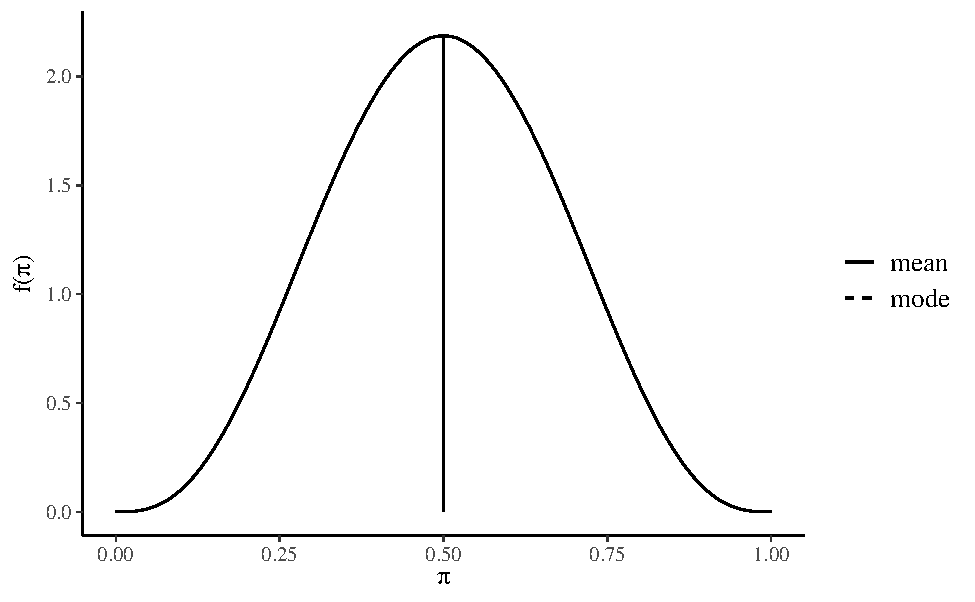
\includegraphics{ds4psy_files/figure-latex/unnamed-chunk-9-1} \end{center}

Possiamo quantificare la nostra incertezza calcolando, con un grado di fiducia del 95\%, la regione nella quale, in base a tale credenza a priori, si trova il valore del parametro. Per ottenere tale intervallo di credibilità a priori, usiamo la funzione \texttt{qbeta()} di \(\R\). In \texttt{qbeta()} i parametri \(\alpha\) e \(\beta\) sono chiamati \texttt{shape1} e \texttt{shape2}:

\begin{Shaded}
\begin{Highlighting}[]
\FunctionTok{qbeta}\NormalTok{(}\FunctionTok{c}\NormalTok{(}\FloatTok{0.025}\NormalTok{, }\FloatTok{0.975}\NormalTok{), }\AttributeTok{shape1 =} \DecValTok{4}\NormalTok{, }\AttributeTok{shape2 =} \DecValTok{4}\NormalTok{)}
\CommentTok{\#\textgreater{} [1] 0.1841 0.8159}
\end{Highlighting}
\end{Shaded}

Se poniamo \(\alpha=10\) e \(\beta=10\), questo corrisponde ad una credenza a priori che sia egualmente probabile per un'aspettativa futura essere distorta negativamente o positivamente,

\begin{Shaded}
\begin{Highlighting}[]
\FunctionTok{plot\_beta}\NormalTok{(}\AttributeTok{alpha =} \DecValTok{10}\NormalTok{, }\AttributeTok{beta =} \DecValTok{10}\NormalTok{, }\AttributeTok{mean =} \ConstantTok{TRUE}\NormalTok{, }\AttributeTok{mode =} \ConstantTok{TRUE}\NormalTok{)}
\end{Highlighting}
\end{Shaded}

\begin{center}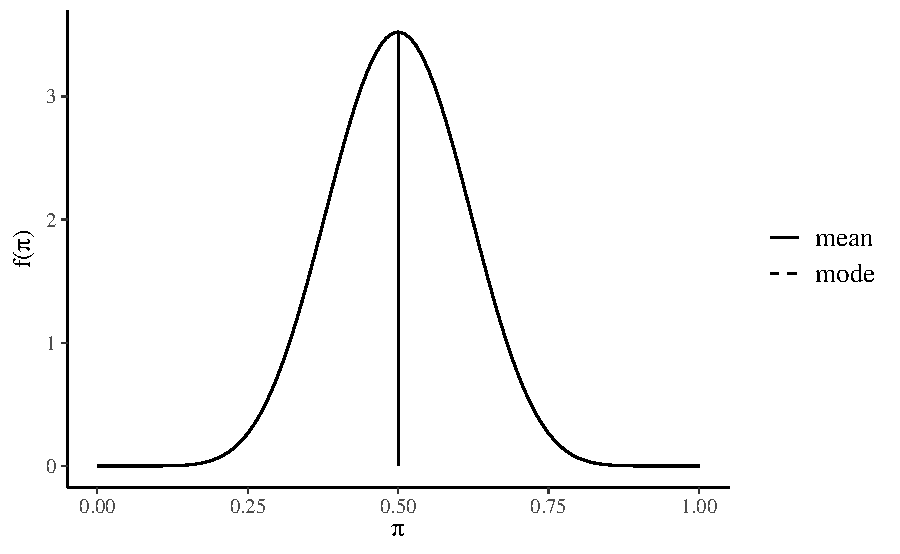
\includegraphics{ds4psy_files/figure-latex/unnamed-chunk-11-1} \end{center}

ma ora la nostra certezza a priori sul valore del parametro è maggiore, come indicato dall'intervallo al 95\%:

\begin{Shaded}
\begin{Highlighting}[]
\FunctionTok{qbeta}\NormalTok{(}\FunctionTok{c}\NormalTok{(}\FloatTok{0.025}\NormalTok{, }\FloatTok{0.975}\NormalTok{), }\AttributeTok{shape1 =} \DecValTok{10}\NormalTok{, }\AttributeTok{shape2 =} \DecValTok{10}\NormalTok{)}
\CommentTok{\#\textgreater{} [1] 0.2886 0.7114}
\end{Highlighting}
\end{Shaded}

Quale distribuzione a priori dobbiamo scegliere? In un problema concreto di analisi dei dati, la scelta della distribuzione a priori dipende dalle credenze a priori che vogliamo includere nell'analisi dei dati. Se non abbiamo alcuna informazione a priori, potremmo usare \(\alpha=1\) e \(\beta=1\), che produce una distribuzione a priori uniforme. Ma l'uso di distribuzioni a priori uniformi è sconsigliato per vari motivi, inclusa l'instabilità numerica della stima dei parametri. È meglio invece usare una distribuzione a priori debolmente informativa, come \(\mbox{Beta}(2, 2)\).

Nella discussione presente, solo per fare un esempio, useremo quale distribuzione a priori una \(\mbox{Beta}(2, 10)\), ovvero:

\[
p(\theta) = \frac{\Gamma(12)}{\Gamma(2)\Gamma(10)}\theta^{2-1} (1-\theta)^{10-1}.
\]

\begin{Shaded}
\begin{Highlighting}[]
\FunctionTok{plot\_beta}\NormalTok{(}\AttributeTok{alpha =} \DecValTok{2}\NormalTok{, }\AttributeTok{beta =} \DecValTok{10}\NormalTok{, }\AttributeTok{mean =} \ConstantTok{TRUE}\NormalTok{, }\AttributeTok{mode =} \ConstantTok{TRUE}\NormalTok{)}
\end{Highlighting}
\end{Shaded}

\begin{center}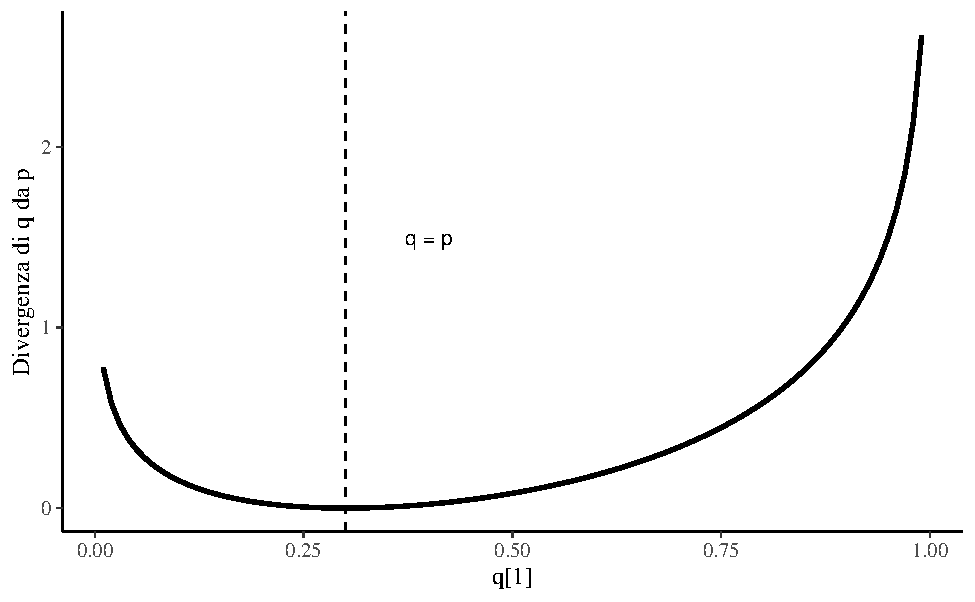
\includegraphics{ds4psy_files/figure-latex/unnamed-chunk-13-1} \end{center}

La \(\mbox{Beta}(2, 10)\) esprime la credenza che \(\theta < 0.5\), con il valore più plausibile pari a cicrca 0.1.

\hypertarget{la-specificazione-della-distribuzione-a-posteriori}{%
\subsection{La specificazione della distribuzione a posteriori}\label{la-specificazione-della-distribuzione-a-posteriori}}

Una volta scelta una distribuzione a priori di tipo Beta, i cui parametri rispecchiano le nostre credenze iniziali su \(\theta\), la distribuzione a posteriori viene specificata dalla formula di Bayes:

\[
\text{distribuzione a posteriori} = \frac{\text{verosimiglianza}\cdot\text{distribuzione a priori}}{\text{verosimiglianza marginale}}.
\]

Nel caso presente abbiamo

\[
p(\theta \mid n=30, y=23) = \frac{\Big[\binom{30}{23}\theta^{23}(1-\theta)^{30-23}\Big]\Big[\frac{\Gamma(12)}{\Gamma(2)\Gamma(10)}\theta^{2-1} (1-\theta)^{10-1}\Big]}{p(y = 23)},
\]

laddove \(p(y = 23)\), ovvero la verosimiglianza marginale, è una costante di normalizzazione.

Riscriviamo l'equazione precedente in termini più generali:

\[
p(\theta \mid n, y) = \frac{\Big[\binom{n}{y}\theta^{y}(1-\theta)^{n-y}\Big]\Big[\frac{\Gamma(a+b)}{\Gamma(a)\Gamma(b)}\theta^{a-1} (1-\theta)^{b-1}\Big]}{p(y)}
\]

Raccogliendo tutte le costanti otteniamo:

\[
p(\theta \mid n, y) =\left[\frac{\binom{n}{y}\frac{\Gamma(a+b)}{\Gamma(a)\Gamma(b)}}{p(y)}\right] \theta^{y}(1-\theta)^{n-y}\theta^{a-1} (1-\theta)^{b-1}.
\]

Se ignoriamo il termine costante all'interno della parentesi quadra

\begin{align}
p(\theta \mid n, y) &\propto \theta^{y}(1-\theta)^{n-y}\theta^{a-1} (1-\theta)^{b-1},\notag\\
&\propto \theta^{a+y-1}(1-\theta)^{b+n-y-1},\notag
\end{align}

il termine di destra dell'equazione precedente identifica il \emph{kernel} della distribuzione a posteriori e corrisponde ad una Beta \emph{non normalizzata} di parametri \(a + y\) e \(b + n - y\).

Per ottenere una distribuzione di densità, dobbiamo aggiungere una costante di normalizzazione al kernel della distribuzione a posteriori. In base alla definizione della distribuzione Beta, ed essendo \(a' = a+y\) e \(b' = b+n-y\), tale costante di normalizzazione sarà uguale a

\[
\frac{\Gamma(a'+b')}{\Gamma(a')\Gamma(b')} = \frac{\Gamma(a+b+n)}{\Gamma(a+y)\Gamma(b+n-y)}.
\]

In altri termini, nel caso dello schema beta-binomiale, la distribuzione a posteriori è una \(\mbox{Beta}(a+y, b+n-y)\):

\[
\mbox{Beta}(a+y, b+n-y) = \frac{\Gamma(a+b+n)}{\Gamma(a+y)\Gamma(b+n-y)} \theta^{a+y-1}(1-\theta)^{b+n-y-1}.
\]

In sintesi, moltiplicando verosimiglianza \(\mbox{Bin}(n = 30, y = 23 \mid \theta)\) per la la distribuzione a priori \(\theta \sim \mbox{Beta}(2, 10)\) e dividendo per la costante di normalizzazione, abbiamo ottenuto la distribuzione a posteriori \(p(\theta \mid n, y) \sim \mbox{Beta}(25, 17)\). Questo è un esempio di analisi coniugata. La presente combinazione di verosimiglianza e distribuzione a priori è chiamata caso coniugato \emph{beta-binomiale} ed è descritta dal seguente teorema.

\begin{theorem}
\protect\hypertarget{thm:post-beta-bin-1}{}\label{thm:post-beta-bin-1}Sia data la funzione di verosimiglianza \(\mbox{Bin}(n, y \mid \theta)\) e sia \(\mbox{Beta}(\alpha, \beta)\) una distribuzione a priori. In tali circostanze, la distribuzione a posteriori del parametro \(\theta\) sarà una distribuzione \(\mbox{Beta}(\alpha + y, \beta + n - y)\).
\end{theorem}

È facile calcolare il valore atteso a posteriori di \(\theta\). Essendo \(\E[\mbox{Beta}(\alpha, \beta)] = \frac{\alpha}{\alpha + \beta}\), il risultato cercato diventa

\begin{equation}
\E_{\text{post}} [\mathrm{Beta}(\alpha + y, \beta + n - y)] = \frac{\alpha + y}{\alpha + \beta +n}.
\label{eq:ev-post-beta-bin-1}
\end{equation}

\begin{exercise}

Si rappresenti in maniera grafica e si descriva in forma numerica l'aggiornamento bayesiano beta-binomiale per i dati di \citet{zetschefuture2019}. Si assuma una distribuzione a priori \(\mbox{Beta}(2, 10)\).

Per i dati in questione, l'aggiornamento bayesiano può essere rappresentato in forma grafica usando la funzione \texttt{plot\_beta\_binomial()} del pacchetto \texttt{bayesrules}:

\begin{Shaded}
\begin{Highlighting}[]
\NormalTok{bayesrules}\SpecialCharTok{::}\FunctionTok{plot\_beta\_binomial}\NormalTok{(}
  \AttributeTok{alpha =} \DecValTok{2}\NormalTok{, }\AttributeTok{beta =} \DecValTok{10}\NormalTok{, }\AttributeTok{y =} \DecValTok{23}\NormalTok{, }\AttributeTok{n =} \DecValTok{30}
\NormalTok{  ) }
\end{Highlighting}
\end{Shaded}

\begin{center}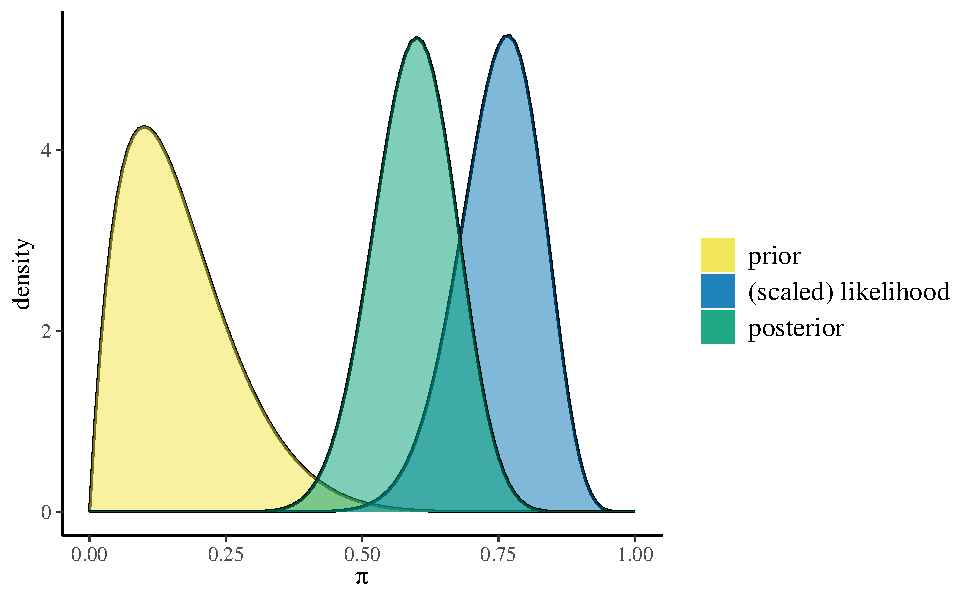
\includegraphics{ds4psy_files/figure-latex/unnamed-chunk-14-1} \end{center}

Oppure, possiamo scrivere noi stessi una funzione, come ad esempio la funzione \texttt{plot\_beta\_binom()} riportata in Appendice \ref{appendix:beta-binom}. Mediante tale la funzione otteniamo

\begin{Shaded}
\begin{Highlighting}[]
\FunctionTok{plot\_beta\_bin}\NormalTok{(}\DecValTok{2}\NormalTok{, }\DecValTok{10}\NormalTok{, }\DecValTok{23}\NormalTok{, }\DecValTok{30}\NormalTok{)}
\end{Highlighting}
\end{Shaded}

\begin{center}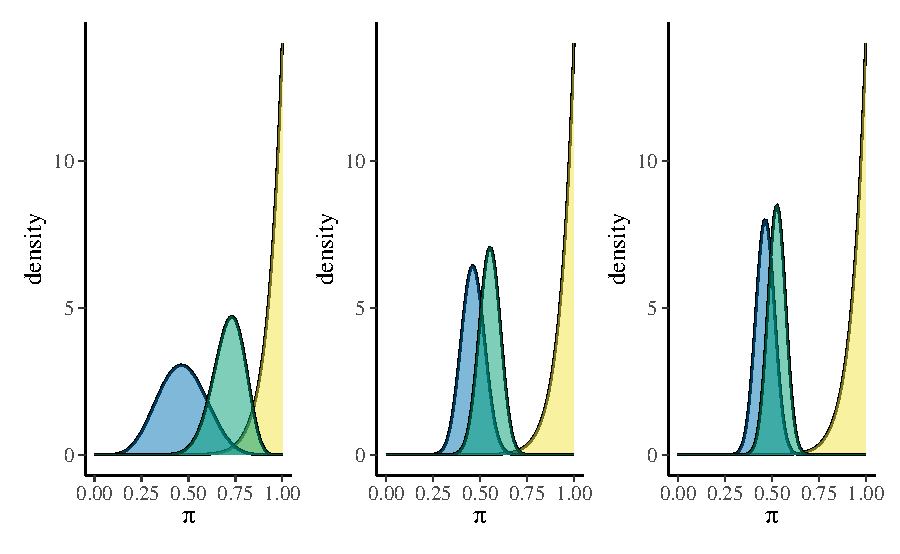
\includegraphics{ds4psy_files/figure-latex/unnamed-chunk-16-1} \end{center}

Un sommario delle distribuzioni a priori e a posteriori può essere ottenuto, ad esempio, usando la funzione \texttt{summarize\_beta\_binomial()} del pacchetto \texttt{bayesrules}:

\begin{Shaded}
\begin{Highlighting}[]
\NormalTok{bayesrules}\SpecialCharTok{:::}\FunctionTok{summarize\_beta\_binomial}\NormalTok{(}
  \AttributeTok{alpha =} \DecValTok{2}\NormalTok{, }\AttributeTok{beta =} \DecValTok{10}\NormalTok{, }\AttributeTok{y =} \DecValTok{23}\NormalTok{, }\AttributeTok{n =} \DecValTok{30}
\NormalTok{)}
\CommentTok{\#\textgreater{}       model alpha beta   mean mode      var      sd}
\CommentTok{\#\textgreater{} 1     prior     2   10 0.1667  0.1 0.010684 0.10336}
\CommentTok{\#\textgreater{} 2 posterior    25   17 0.5952  0.6 0.005603 0.07485}
\end{Highlighting}
\end{Shaded}

\end{exercise}

\begin{exercise}

Per i dati di \citet{zetschefuture2019}, si trovino la media, la moda, la deviazione standard della distribuzione a posteriori di \(\theta\). Si trovi inoltre l'intervallo di credibilità a posteriori del 95\% per il parametro \(\theta\).

Usando il Teorema \ref{thm:post-beta-bin-1}, l'intervallo di credibilità a posteriori del 95\% per il parametro \(\theta\) è:

\begin{Shaded}
\begin{Highlighting}[]
\FunctionTok{qbeta}\NormalTok{(}\FunctionTok{c}\NormalTok{(}\FloatTok{0.025}\NormalTok{, }\FloatTok{0.975}\NormalTok{), }\AttributeTok{shape1 =} \DecValTok{25}\NormalTok{, }\AttributeTok{shape2 =} \DecValTok{17}\NormalTok{)}
\CommentTok{\#\textgreater{} [1] 0.4450 0.7368}
\end{Highlighting}
\end{Shaded}

Usando la \eqref{eq:ev-post-beta-bin-1}, la media della distribuzione a posteriori è

\begin{Shaded}
\begin{Highlighting}[]
\DecValTok{25} \SpecialCharTok{/}\NormalTok{ (}\DecValTok{25} \SpecialCharTok{+} \DecValTok{17}\NormalTok{)}
\CommentTok{\#\textgreater{} [1] 0.5952}
\end{Highlighting}
\end{Shaded}

Per le proprietà della distribuzione Beta, la moda della distribuzione a posteriori è

\begin{Shaded}
\begin{Highlighting}[]
\NormalTok{(}\DecValTok{25} \SpecialCharTok{{-}} \DecValTok{1}\NormalTok{) }\SpecialCharTok{/}\NormalTok{ (}\DecValTok{25} \SpecialCharTok{+} \DecValTok{17} \SpecialCharTok{{-}} \DecValTok{2}\NormalTok{)}
\CommentTok{\#\textgreater{} [1] 0.6}
\end{Highlighting}
\end{Shaded}

e la deviazione standard della distribuzione a priori è

\begin{Shaded}
\begin{Highlighting}[]
\FunctionTok{sqrt}\NormalTok{((}\DecValTok{25} \SpecialCharTok{*} \DecValTok{17}\NormalTok{) }\SpecialCharTok{/}\NormalTok{ ((}\DecValTok{25} \SpecialCharTok{+} \DecValTok{17}\NormalTok{)}\SpecialCharTok{\^{}}\DecValTok{2} \SpecialCharTok{*}\NormalTok{ (}\DecValTok{25} \SpecialCharTok{+} \DecValTok{17} \SpecialCharTok{+} \DecValTok{1}\NormalTok{)))}
\CommentTok{\#\textgreater{} [1] 0.07485}
\end{Highlighting}
\end{Shaded}

\end{exercise}

\begin{exercise}

Si trovino i parametri e le proprietà della distribuzione a posteriori del parametro \(\theta\) per i dati dell'esempio relativo alla ricerca di Stanley Milgram discussa da \citet{Johnson2022bayesrules}.

Nel 1963, Stanley Milgram presentò una ricerca sulla propensione delle persone a obbedire agli ordini di figure di autorità, anche quando tali ordini possono danneggiare altre persone \citep{milgram1963behavioral}. Nell'articolo, Milgram descrive lo studio come \emph{``consist{[}ing{]} of ordering a naive subject to administer electric shock to a victim. A simulated shock generator is used, with 30 clearly marked voltage levels that range from IS to 450 volts. The instrument bears verbal designations that range from Slight Shock to Danger: Severe Shock. The responses of the victim, who is a trained confederate of the experimenter, are standardized. The orders to administer shocks are given to the naive subject in the context of a `learning experiment' ostensibly set up to study the effects of punishment on memory. As the experiment proceeds the naive subject is commanded to administer increasingly more intense shocks to the victim, even to the point of reaching the level marked Danger: Severe Shock.''}

All'insaputa del partecipante, gli shock elettrici erano falsi e l'attore stava solo fingendo di provare il dolore dello shock.

\citet{Johnson2022bayesrules} fanno inferenza sui risultati dello studio di Milgram mediante il modello Beta-Binomiale. Il parametro di interesse è \(\theta\), la probabiltà che una persona obbedisca all'autorità (in questo caso, somministrando lo shock più severo), anche se ciò significa recare danno ad altri. \citet{Johnson2022bayesrules} ipotizzano che, prima di raccogliere dati, le credenze di Milgram relative a \(\theta\) possano essere rappresentate mediante una \(\mbox{Beta}(1, 10)\). Sia \(y = 26\) il numero di soggetti che, sui 40 partecipanti allo studio, aveva accettato di infliggere lo shock più severo. Assumendo che ogni partecipante si comporti indipendentemente dagli altri, possiamo modellare la dipendenza di \(y\) da \(\theta\) usando la distribuzione binomiale. Giungiamo dunque al seguente modello bayesiano Beta-Binomiale:

\begin{align}
y \mid \theta & \sim \mbox{Bin}(n = 40, \theta) \notag\\
\theta & \sim \text{Beta}(1, 10) \; . \notag
\end{align}

Usando le funzioni di \texttt{bayesrules} possiamo facilmente calcolare i parametri e le proprietà della distribuzione a posteriori:

\begin{Shaded}
\begin{Highlighting}[]
\NormalTok{bayesrules}\SpecialCharTok{:::}\FunctionTok{summarize\_beta\_binomial}\NormalTok{(}
  \AttributeTok{alpha =} \DecValTok{1}\NormalTok{, }\AttributeTok{beta =} \DecValTok{10}\NormalTok{, }\AttributeTok{y =} \DecValTok{26}\NormalTok{, }\AttributeTok{n =} \DecValTok{40}
\NormalTok{)}
\CommentTok{\#\textgreater{}       model alpha beta    mean   mode      var      sd}
\CommentTok{\#\textgreater{} 1     prior     1   10 0.09091 0.0000 0.006887 0.08299}
\CommentTok{\#\textgreater{} 2 posterior    27   24 0.52941 0.5306 0.004791 0.06922}
\end{Highlighting}
\end{Shaded}

Il processo di aggiornamento bayesiano è descritto dalla figura seguente:

\begin{Shaded}
\begin{Highlighting}[]
\FunctionTok{plot\_beta\_bin}\NormalTok{(}\DecValTok{1}\NormalTok{, }\DecValTok{10}\NormalTok{, }\DecValTok{26}\NormalTok{, }\DecValTok{40}\NormalTok{)}
\end{Highlighting}
\end{Shaded}

\begin{center}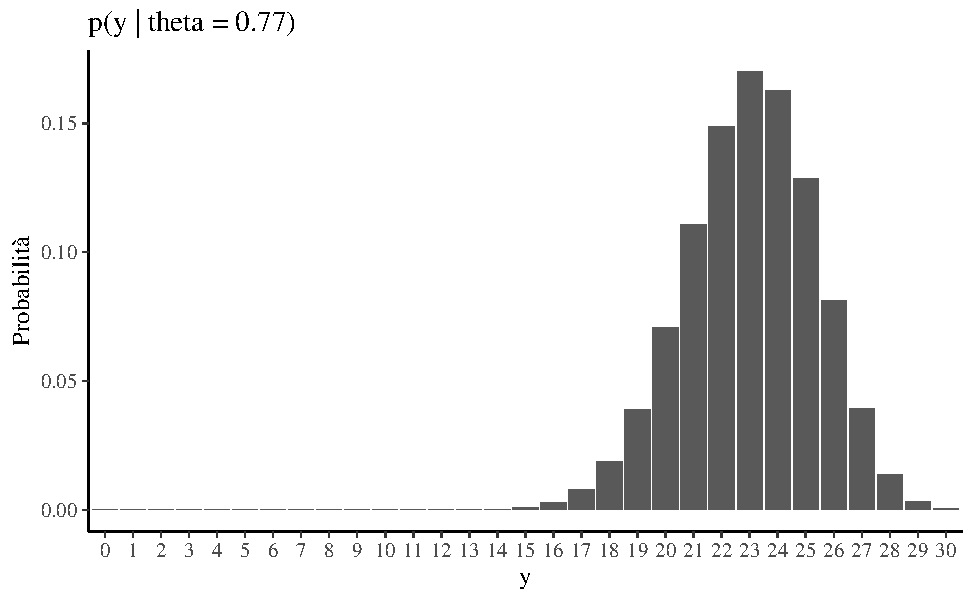
\includegraphics{ds4psy_files/figure-latex/unnamed-chunk-23-1} \end{center}

\end{exercise}

\hypertarget{principali-distribuzioni-coniugate}{%
\section{Principali distribuzioni coniugate}\label{principali-distribuzioni-coniugate}}

Esistono molte altre combinazioni simili di verosimiglianza e distribuzione a priori le quali producono una distribuzione a posteriori che ha la stessa densità della distribuzione a priori. Sono elencate qui sotto le più note coniugazioni tra modelli statistici e distribuzioni a priori.

\begin{itemize}
\tightlist
\item
  Per il modello Normale-Normale \(\mathcal{N}(\mu, \sigma^2_0)\), la distribizione iniziale è \(\mathcal{N}(\mu_0, \tau^2)\) e la distribuzione finale è \(\mathcal{N}\left(\frac{\mu_0\sigma^2 + \bar{y}n\tau^2}{\sigma^2 + n\tau^2}, \frac{\sigma^2\tau^2}{\sigma^2 + n\tau^2} \right)\).
\item
  Per il modello Poisson-gamma \(\text{Po}(\theta)\), la distribizione iniziale è \(\Gamma(\lambda, \delta)\) e la distribuzione finale è \(\Gamma(\lambda + n \bar{y}, \delta +n)\).
\item
  Per il modello esponenziale \(\text{Exp}(\theta)\), la distribizione iniziale è \(\Gamma(\lambda, \delta)\) e la distribuzione finale è \(\Gamma(\lambda + n, \delta +n\bar{y})\).
\item
  Per il modello uniforme-Pareto \(\text{U}(0, \theta)\), la distribizione iniziale è \(\mbox{Pa}(\alpha, \varepsilon)\) e la distribuzione finale è \(\mbox{Pa}(\alpha + n, \max(y_{(n)}, \varepsilon))\).
\end{itemize}

\hypertarget{commenti-e-considerazioni-finali-1}{%
\section*{Commenti e considerazioni finali}\label{commenti-e-considerazioni-finali-1}}


Lo scopo di questa discussione è mostrare come sia possibile combinare le nostre conoscenze a priori (espresse nei termini di una densità di probabilità) con le evidenze fornite dai dati (espresse nei termini della funzione di verosimiglianza), così da determinare, mediante il teorema di Bayes, una distribuzione a posteriori, la quale condensa l'incertezza che abbiamo sul parametro \(\theta\). Per illustrare tale problema, abbiamo considerato una situazione nella quale \(\theta\) corrisponde alla probabilità di successo in una sequenza di prove Bernoulliane. In tali circostanze è ragionevole esprimere le nostre credenze a priori mediante la densità Beta, con opportuni parametri. L'inferenza rispetto a \(\theta\) può essere svolta utilizzando una distribuzione a priori Beta e una verosimiglianza binomiale. Così facendo, la distribuzione a posteriori diventa essa stessa una distribuzione Beta -- questo è il cosiddetto schema beta-binomiale. Dato che utilizza una distribuzione a priori coniugata, lo schema beta-binomiale rende possibile la determinazione analitica dei parametri della distribuzione a posteriori.

\hypertarget{chapter-balance}{%
\chapter{L'influenza della distribuzione a priori}\label{chapter-balance}}

La notazione \(p(\theta \mid y) \propto p(\theta) \ p(y \mid \theta)\) rende particolarmente chiaro che la distribuzione a posteriori è un ``miscuglio'' della distribuzione a priori e della verosimiglianza. Prima di preoccuparci di come calcolare la distribuzione a posteriori, cerchiamo di capire meglio cosa significa ``mescolare'' la distribuzione a priori e la verosimiglianza. Considereremo qui un esempio discusso da \citet{Johnson2022bayesrules}.

\hypertarget{il-test-di-benchdel}{%
\section{Il test di Benchdel}\label{il-test-di-benchdel}}

Nel fumetto di Alison Bechdel \emph{The Rule}, un personaggio afferma di guardare un film solo se soddisfa le seguenti tre regole \citep{Bechdel1986dykes}:

\begin{itemize}
\tightlist
\item
  almeno due caratteri nel film devono essere donne;
\item
  queste due donne si parlano;
\item
  parlano di qualcosa altro oltre a parlare di qualche uomo.
\end{itemize}

Questi criteri costituiscono il \emph{test di Bechdel} per la rappresentazione delle donne nei film. \citet{Johnson2022bayesrules} pongono la seguente domanda ``Quale percentuale dei film che avete visto supera il test di Bechdel?''.

Sia \(\pi \in [0, 1]\) una variabile casuale che indica la proporzione sconosciuta di film che superano il test di Bechdel. Tre amiche --- la femminista, l'ignara e l'ottimista --- hanno opionioni diverse su \(\pi\). Riflettendo sui film che ha visto, la femminista capisce che nella maggioranza dei film mancano personaggi femminili forti. L'ignara non ricorda bene i film che ha visto, quindi non sa quanti film superano il test di Bechdel. Infine, l'ottimista pensa che, in generale, le donne sono ben rappresentate all'interno dei film: secondo lei quasi tutti i film superano il test di Bechdel. Le tre amiche hanno dunque tre modelli a priori diversi di \(\pi\).

Abbiamo visto in precedenza come sia possibile usare la distribuzione Beta per rappresentare le credenze a priori. Ponendo la gran parte della massa della probabilità a priori su valori \(\pi < 0.5\), la distribuzione a priori \(\text{Beta}(5, 11)\) riflette il punto di vista femminista secondo il quale la maggioranza dei film non supera il test di Bechdel. Al contrario, la \(\text{Beta}(14,1)\) pone la gran parte della massa della distribuzione a priori su valori \(\pi\) prossimi a 1, e corrisponde quindi alle credenze a priori dell'amica ottimista. Infine, una \(\text{Beta}(1 ,1)\) o \(Unif(0, 1)\), assegna lo stesso livello di plausibilità a tutti i valori \(\pi \in [0, 1]\), e corrisponde all'incertezza a priori dell'ignara.

Nell'esempio di \citet{Johnson2022bayesrules}, le tre amiche decidono di rivedere un campione di \(n\) film e di registrare \(y\), ovvero il numero di film che superano il test di Bechdel. Se \(y\) corrisponde al numero di ``successi'' in un numero fisso di \(n\) prove Bernoulliane i.i.d., allora la dipendenza di \(y\) da \(\pi\) viene specificata nei termini di un modello binomiale. Quindi, per ciascuna delle tre amiche è possibile scrivere un modello beta-binomiale

\begin{align}
Y \mid \pi & \sim \mbox{Bin}(n, \pi)  \notag\\
\pi & \sim \mbox{Beta}(\alpha, \beta) \notag
\end{align}

che utilizza diversi parametri \(\alpha\) e \(\beta\) per la distribuzione a priori e che conduce a tre diverse distribuzioni a posteriori per il parametro sconosciuto \(\pi\):

\begin{equation}
\pi \mid (Y = y) \sim \mbox{Beta}(\alpha + y, \beta + n - y).
\end{equation}

\citet{Johnson2022bayesrules} si chiedono come le credenze a priori delle tre amiche influenzano le conclusioni a posteriori a cui esse giungono, dopo avere osservato i dati. Si chiedono inoltre in che modo la dimensione del campione moduli l'influenza della distribuzione a priori sulla distribuzione a posteriori. Per rispondere a queste domande, \citet{Johnson2022bayesrules} consideriamo tre diversi scenari:

\begin{itemize}
\tightlist
\item
  gli stessi dati osservati, ma distribuzioni a priori diverse;
\item
  dati diversi, ma la stessa distribuzione a priori;
\item
  dati diversi e distribuzioni a priori diverse.
\end{itemize}

\hypertarget{stessi-dati-ma-diverse-distribuzioni-a-priori}{%
\section{Stessi dati ma diverse distribuzioni a priori}\label{stessi-dati-ma-diverse-distribuzioni-a-priori}}

Iniziamo con lo scenario che descrive il caso in cui abbiamo gli stessi dati ma diverse distribuzioni a priori. Supponiamo che le tre amiche decidano di guardare insieme 20 film selezionati a caso:

\begin{Shaded}
\begin{Highlighting}[]
\FunctionTok{data}\NormalTok{(bechdel, }\AttributeTok{package =} \StringTok{"bayesrules"}\NormalTok{)}
\FunctionTok{set.seed}\NormalTok{(}\DecValTok{84735}\NormalTok{)}
\NormalTok{bechdel\_20 }\OtherTok{\textless{}{-}}\NormalTok{ bechdel }\SpecialCharTok{\%\textgreater{}\%} 
  \FunctionTok{sample\_n}\NormalTok{(}\DecValTok{20}\NormalTok{)}
\NormalTok{bechdel\_20 }\SpecialCharTok{\%\textgreater{}\%} 
  \FunctionTok{head}\NormalTok{(}\DecValTok{3}\NormalTok{)}
\CommentTok{\#\textgreater{} \# A tibble: 3 x 3}
\CommentTok{\#\textgreater{}    year title      binary}
\CommentTok{\#\textgreater{}   \textless{}dbl\textgreater{} \textless{}chr\textgreater{}      \textless{}chr\textgreater{} }
\CommentTok{\#\textgreater{} 1  2005 King Kong  FAIL  }
\CommentTok{\#\textgreater{} 2  1983 Flashdance PASS  }
\CommentTok{\#\textgreater{} 3  2013 The Purge  FAIL}
\end{Highlighting}
\end{Shaded}

\noindent Di questi 20 film, solo il 45\% (\(y\) = 9) passa il test di Bechdel:

\begin{Shaded}
\begin{Highlighting}[]
\NormalTok{bechdel\_20 }\SpecialCharTok{\%\textgreater{}\%} 
\NormalTok{  janitor}\SpecialCharTok{::}\FunctionTok{tabyl}\NormalTok{(binary) }\SpecialCharTok{\%\textgreater{}\%} 
\NormalTok{  janitor}\SpecialCharTok{::}\FunctionTok{adorn\_totals}\NormalTok{(}\StringTok{"row"}\NormalTok{)}
\CommentTok{\#\textgreater{}  binary  n percent}
\CommentTok{\#\textgreater{}    FAIL 11    0.55}
\CommentTok{\#\textgreater{}    PASS  9    0.45}
\CommentTok{\#\textgreater{}   Total 20    1.00}
\end{Highlighting}
\end{Shaded}

Esaminiamo ora le tre distribuzioni a posteriori. Per la femminista abbiamo:

\begin{Shaded}
\begin{Highlighting}[]
\NormalTok{bayesrules}\SpecialCharTok{:::}\FunctionTok{plot\_beta\_binomial}\NormalTok{(}
  \AttributeTok{alpha =} \DecValTok{5}\NormalTok{, }\AttributeTok{beta =} \DecValTok{11}\NormalTok{, }\AttributeTok{y =} \DecValTok{9}\NormalTok{, }\AttributeTok{n =} \DecValTok{20}
\NormalTok{  ) }
\end{Highlighting}
\end{Shaded}

\begin{center}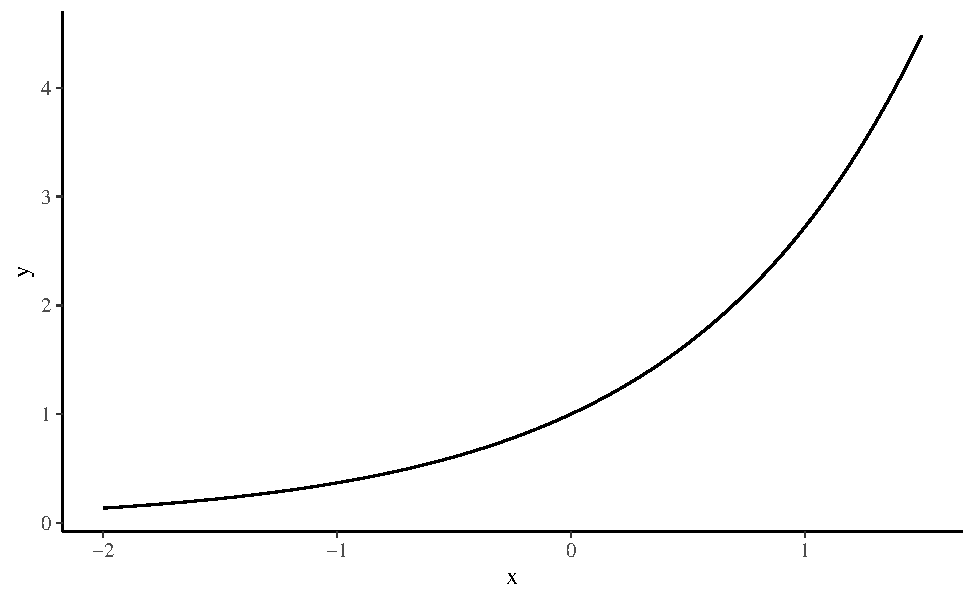
\includegraphics{ds4psy_files/figure-latex/unnamed-chunk-26-1} \end{center}

\begin{Shaded}
\begin{Highlighting}[]
\NormalTok{bayesrules}\SpecialCharTok{:::}\FunctionTok{summarize\_beta\_binomial}\NormalTok{(}
  \AttributeTok{alpha =} \DecValTok{5}\NormalTok{, }\AttributeTok{beta =} \DecValTok{11}\NormalTok{, }\AttributeTok{y =} \DecValTok{9}\NormalTok{, }\AttributeTok{n =} \DecValTok{20}
\NormalTok{)}
\CommentTok{\#\textgreater{}       model alpha beta   mean   mode      var      sd}
\CommentTok{\#\textgreater{} 1     prior     5   11 0.3125 0.2857 0.012638 0.11242}
\CommentTok{\#\textgreater{} 2 posterior    14   22 0.3889 0.3824 0.006423 0.08014}
\end{Highlighting}
\end{Shaded}

Per l'ottimista abbiamo:

\begin{Shaded}
\begin{Highlighting}[]
\NormalTok{bayesrules}\SpecialCharTok{:::}\FunctionTok{plot\_beta\_binomial}\NormalTok{(}
  \AttributeTok{alpha =} \DecValTok{14}\NormalTok{, }\AttributeTok{beta =} \DecValTok{1}\NormalTok{, }\AttributeTok{y =} \DecValTok{9}\NormalTok{, }\AttributeTok{n =} \DecValTok{20}
\NormalTok{) }
\end{Highlighting}
\end{Shaded}

\begin{center}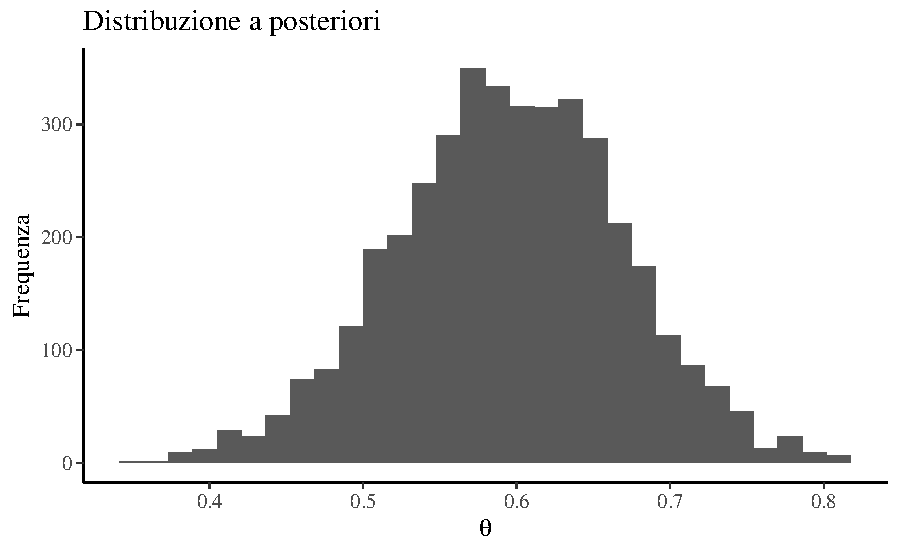
\includegraphics{ds4psy_files/figure-latex/unnamed-chunk-28-1} \end{center}

\begin{Shaded}
\begin{Highlighting}[]
\NormalTok{bayesrules}\SpecialCharTok{:::}\FunctionTok{summarize\_beta\_binomial}\NormalTok{(}
  \AttributeTok{alpha =} \DecValTok{14}\NormalTok{, }\AttributeTok{beta =} \DecValTok{1}\NormalTok{, }\AttributeTok{y =} \DecValTok{9}\NormalTok{, }\AttributeTok{n =} \DecValTok{20}
\NormalTok{)}
\CommentTok{\#\textgreater{}       model alpha beta   mean   mode      var      sd}
\CommentTok{\#\textgreater{} 1     prior    14    1 0.9333 1.0000 0.003889 0.06236}
\CommentTok{\#\textgreater{} 2 posterior    23   12 0.6571 0.6667 0.006259 0.07911}
\end{Highlighting}
\end{Shaded}

Infine, per l'ignara troviamo

\begin{Shaded}
\begin{Highlighting}[]
\NormalTok{bayesrules}\SpecialCharTok{:::}\FunctionTok{plot\_beta\_binomial}\NormalTok{(}
  \AttributeTok{alpha =} \DecValTok{1}\NormalTok{, }\AttributeTok{beta =} \DecValTok{1}\NormalTok{, }\AttributeTok{y =} \DecValTok{9}\NormalTok{, }\AttributeTok{n =} \DecValTok{20}
\NormalTok{)}
\end{Highlighting}
\end{Shaded}

\begin{center}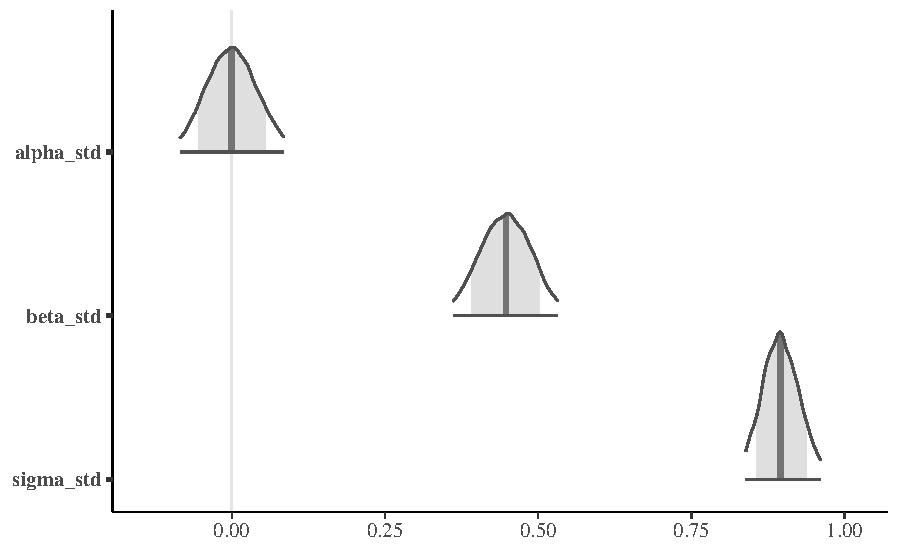
\includegraphics{ds4psy_files/figure-latex/unnamed-chunk-30-1} \end{center}

\begin{Shaded}
\begin{Highlighting}[]
\NormalTok{bayesrules}\SpecialCharTok{:::}\FunctionTok{summarize\_beta\_binomial}\NormalTok{(}
  \AttributeTok{alpha =} \DecValTok{1}\NormalTok{, }\AttributeTok{beta =} \DecValTok{1}\NormalTok{, }\AttributeTok{y =} \DecValTok{9}\NormalTok{, }\AttributeTok{n =} \DecValTok{20}
\NormalTok{)}
\CommentTok{\#\textgreater{}       model alpha beta   mean mode     var     sd}
\CommentTok{\#\textgreater{} 1     prior     1    1 0.5000  NaN 0.08333 0.2887}
\CommentTok{\#\textgreater{} 2 posterior    10   12 0.4545 0.45 0.01078 0.1038}
\end{Highlighting}
\end{Shaded}

Per calcolare la distribuzione a posteriori, ho qui usato le funzioni del pacchetto \texttt{bayesrules}. Ma per lo schema beta-binomiale è facile trovare i parametri della distribuzione a posteriori. Per esempio, nel caso dell'amica femminista, la distribuzione a posteriori è una Beta di parametri

\[
\alpha_{post} = \alpha_{prior} + y = 5+9 = 14
\] e

\[
\beta_{post} = \beta_{prior} + n - y = 11 + 20 - 9 = 22.
\]

L'aggiornamento bayesiano indica che le tre amiche ottengono valori per la media (o la moda) a posteriori per \(\pi\) molto diversi. Dunque, anche dopo avere visto 20 film, le tre amiche non si trovano d'accordo su quale sia la proporzione di film che passano il test di Bechdel.

Questo non dovrebbe sorprenderci. L'amica ottimista aveva opinioni molto forti sul valore di \(\pi\) e i \emph{pochi} nuovi dati che le sono stati forniti non sono riusciti a convincerla a cambiare idea: crede ancora che i valori \(\pi > 0.5\) siano i più plausibili. Lo stesso si può dire, all'estremo opposto, dell'amica femminista: anche lei continua a credere che i valori \(\pi < =.5\) siano i più plausibili. Infine, l'ignara non aveva nessuna opinione a priori su \(\pi\) e, anche dopo avere visto 20 film, continua a credere che il valore \(\pi\) più plausibile sia quello intermedio, nell'intorno di 0.5.

\hypertarget{dati-diversi-ma-la-stessa-distribuzione-a-priori}{%
\section{Dati diversi ma la stessa distribuzione a priori}\label{dati-diversi-ma-la-stessa-distribuzione-a-priori}}

Supponiamo ora che l'amica ottimista abbia tre amiche, Maria, Anna e Sara, tutte ottimiste come lei. L'ottimista chiede a Maria, Anna e Sara di fare loro stesse l'esperimento descritto in precedenza. Maria guarda 13 film; di questi 6 passano il test di Bechdel. Anna guarda 63 film; di questi 29 passano il test di Bechdel. Sara guarda 99 film; di questi 46 passano il test di Bechdel.

Supponiamo che Maria, Anna e Sara condividano la stessa credenza a priori su \(\pi\): ovvero, Beta(14, 1). In tali circostanze e, alla luce dei dati osservati, cosa possiamo dire delle tre distribuzioni a posteriori?

\begin{Shaded}
\begin{Highlighting}[]
\NormalTok{p1 }\OtherTok{\textless{}{-}}\NormalTok{ bayesrules}\SpecialCharTok{:::}\FunctionTok{plot\_beta\_binomial}\NormalTok{(}
  \AttributeTok{alpha =} \DecValTok{14}\NormalTok{, }\AttributeTok{beta =} \DecValTok{1}\NormalTok{, }\AttributeTok{y =} \DecValTok{6}\NormalTok{, }\AttributeTok{n =} \DecValTok{13}
\NormalTok{  ) }\SpecialCharTok{+} 
  \FunctionTok{theme}\NormalTok{(}\AttributeTok{legend.position =} \StringTok{"none"}\NormalTok{) }
\NormalTok{p2 }\OtherTok{\textless{}{-}}\NormalTok{ bayesrules}\SpecialCharTok{:::}\FunctionTok{plot\_beta\_binomial}\NormalTok{(}
  \AttributeTok{alpha =} \DecValTok{14}\NormalTok{, }\AttributeTok{beta =} \DecValTok{1}\NormalTok{, }\AttributeTok{y =} \DecValTok{29}\NormalTok{, }\AttributeTok{n =} \DecValTok{63}
\NormalTok{  ) }\SpecialCharTok{+} 
  \FunctionTok{theme}\NormalTok{(}\AttributeTok{legend.position =} \StringTok{"none"}\NormalTok{) }
\NormalTok{p3 }\OtherTok{\textless{}{-}}\NormalTok{ bayesrules}\SpecialCharTok{:::}\FunctionTok{plot\_beta\_binomial}\NormalTok{(}
  \AttributeTok{alpha =} \DecValTok{14}\NormalTok{, }\AttributeTok{beta =} \DecValTok{1}\NormalTok{, }\AttributeTok{y =} \DecValTok{46}\NormalTok{, }\AttributeTok{n =} \DecValTok{99}
\NormalTok{  ) }\SpecialCharTok{+}
  \FunctionTok{theme}\NormalTok{(}\AttributeTok{legend.position =} \StringTok{"none"}\NormalTok{) }
\NormalTok{p1 }\SpecialCharTok{+}\NormalTok{ p2 }\SpecialCharTok{+}\NormalTok{ p3}
\end{Highlighting}
\end{Shaded}

\begin{figure}[h]

{\centering 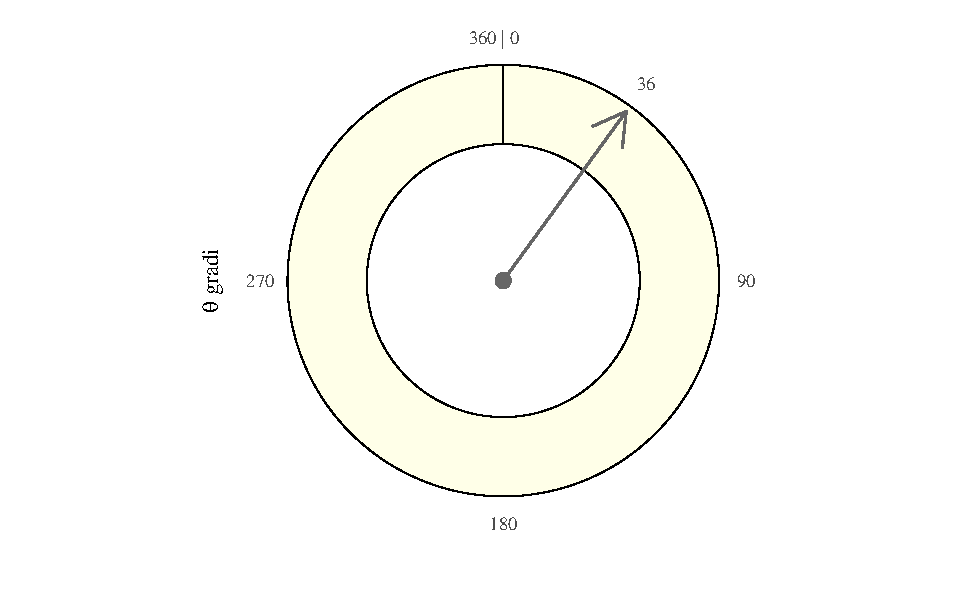
\includegraphics[width=0.95\linewidth]{ds4psy_files/figure-latex/unnamed-chunk-32-1} 

}

\caption{Aggiornamento bayesiano per le credenze di Maria, Anna e Sara.}\label{fig:unnamed-chunk-32}
\end{figure}

Notiamo due cose. All'aumentare delle informazioni disponibili (ovvero, all'aumentare dell'ampiezza del campione), la distribuzione a posteriori si allontana sempre di più dalla distribuzione a priori, e si avvicina sempre di più alla verosimiglianza. In secondo luogo, all'aumentare dell'ampiezza del campione la varianza della distribuzione a posteriori diminuisce sempre di più --- ovvero, diminuisce l'incertezza su quelli che sono i valori \(\pi\) più plausibili.

\hypertarget{dati-diversi-e-diverse-distribuzioni-a-priori}{%
\section{Dati diversi e diverse distribuzioni a priori}\label{dati-diversi-e-diverse-distribuzioni-a-priori}}

Nella figura successiva esaminiamo le distribuzioni a posteriori che si ottengono incrociando tre diversi set di dati (\(y\) = 6, \(n\) = 13;, \(y\) = 29, \(n\) = 63; \(y\) = 66, \(n\) = 99) con tre diverse distribuzioni a priori {[}Beta(14, 1), Beta(5, 11), Beta(1, 1){]}.

\begin{Shaded}
\begin{Highlighting}[]
\NormalTok{p1 }\OtherTok{\textless{}{-}}\NormalTok{ bayesrules}\SpecialCharTok{:::}\FunctionTok{plot\_beta\_binomial}\NormalTok{(}
  \AttributeTok{alpha =} \DecValTok{14}\NormalTok{, }\AttributeTok{beta =} \DecValTok{1}\NormalTok{, }\AttributeTok{y =} \DecValTok{6}\NormalTok{, }\AttributeTok{n =} \DecValTok{13}
\NormalTok{  ) }\SpecialCharTok{+}
  \FunctionTok{theme}\NormalTok{(}\AttributeTok{legend.position =} \StringTok{"none"}\NormalTok{) }
\NormalTok{p2 }\OtherTok{\textless{}{-}}\NormalTok{ bayesrules}\SpecialCharTok{:::}\FunctionTok{plot\_beta\_binomial}\NormalTok{(}
  \AttributeTok{alpha =} \DecValTok{14}\NormalTok{, }\AttributeTok{beta =} \DecValTok{1}\NormalTok{, }\AttributeTok{y =} \DecValTok{29}\NormalTok{, }\AttributeTok{n =} \DecValTok{63}
\NormalTok{  ) }\SpecialCharTok{+}
  \FunctionTok{theme}\NormalTok{(}\AttributeTok{legend.position =} \StringTok{"none"}\NormalTok{) }
\NormalTok{p3 }\OtherTok{\textless{}{-}}\NormalTok{ bayesrules}\SpecialCharTok{:::}\FunctionTok{plot\_beta\_binomial}\NormalTok{(}
  \AttributeTok{alpha =} \DecValTok{14}\NormalTok{, }\AttributeTok{beta =} \DecValTok{1}\NormalTok{, }\AttributeTok{y =} \DecValTok{46}\NormalTok{, }\AttributeTok{n =} \DecValTok{99}
\NormalTok{  ) }\SpecialCharTok{+}
  \FunctionTok{theme}\NormalTok{(}\AttributeTok{legend.position =} \StringTok{"none"}\NormalTok{) }
\NormalTok{p4 }\OtherTok{\textless{}{-}}\NormalTok{ bayesrules}\SpecialCharTok{:::}\FunctionTok{plot\_beta\_binomial}\NormalTok{(}
  \AttributeTok{alpha =} \DecValTok{5}\NormalTok{, }\AttributeTok{beta =} \DecValTok{11}\NormalTok{, }\AttributeTok{y =} \DecValTok{6}\NormalTok{, }\AttributeTok{n =} \DecValTok{13}
\NormalTok{  ) }\SpecialCharTok{+}
  \FunctionTok{theme}\NormalTok{(}\AttributeTok{legend.position =} \StringTok{"none"}\NormalTok{) }
\NormalTok{p5 }\OtherTok{\textless{}{-}}\NormalTok{ bayesrules}\SpecialCharTok{:::}\FunctionTok{plot\_beta\_binomial}\NormalTok{(}
  \AttributeTok{alpha =} \DecValTok{5}\NormalTok{, }\AttributeTok{beta =} \DecValTok{11}\NormalTok{, }\AttributeTok{y =} \DecValTok{29}\NormalTok{, }\AttributeTok{n =} \DecValTok{63}
\NormalTok{  ) }\SpecialCharTok{+}
  \FunctionTok{theme}\NormalTok{(}\AttributeTok{legend.position =} \StringTok{"none"}\NormalTok{) }
\NormalTok{p6 }\OtherTok{\textless{}{-}}\NormalTok{ bayesrules}\SpecialCharTok{:::}\FunctionTok{plot\_beta\_binomial}\NormalTok{(}
  \AttributeTok{alpha =} \DecValTok{5}\NormalTok{, }\AttributeTok{beta =} \DecValTok{11}\NormalTok{, }\AttributeTok{y =} \DecValTok{46}\NormalTok{, }\AttributeTok{n =} \DecValTok{99}
\NormalTok{  ) }\SpecialCharTok{+}
  \FunctionTok{theme}\NormalTok{(}\AttributeTok{legend.position =} \StringTok{"none"}\NormalTok{) }
\NormalTok{p7 }\OtherTok{\textless{}{-}}\NormalTok{ bayesrules}\SpecialCharTok{:::}\FunctionTok{plot\_beta\_binomial}\NormalTok{(}
  \AttributeTok{alpha =} \DecValTok{1}\NormalTok{, }\AttributeTok{beta =} \DecValTok{1}\NormalTok{, }\AttributeTok{y =} \DecValTok{6}\NormalTok{, }\AttributeTok{n =} \DecValTok{13}
\NormalTok{  ) }\SpecialCharTok{+}
  \FunctionTok{theme}\NormalTok{(}\AttributeTok{legend.position =} \StringTok{"none"}\NormalTok{) }
\NormalTok{p8 }\OtherTok{\textless{}{-}}\NormalTok{ bayesrules}\SpecialCharTok{:::}\FunctionTok{plot\_beta\_binomial}\NormalTok{(}
  \AttributeTok{alpha =} \DecValTok{1}\NormalTok{, }\AttributeTok{beta =} \DecValTok{1}\NormalTok{, }\AttributeTok{y =} \DecValTok{29}\NormalTok{, }\AttributeTok{n =} \DecValTok{63}
\NormalTok{  ) }\SpecialCharTok{+}
  \FunctionTok{theme}\NormalTok{(}\AttributeTok{legend.position =} \StringTok{"none"}\NormalTok{) }
\NormalTok{p9 }\OtherTok{\textless{}{-}}\NormalTok{ bayesrules}\SpecialCharTok{:::}\FunctionTok{plot\_beta\_binomial}\NormalTok{(}
  \AttributeTok{alpha =} \DecValTok{1}\NormalTok{, }\AttributeTok{beta =} \DecValTok{1}\NormalTok{, }\AttributeTok{y =} \DecValTok{46}\NormalTok{, }\AttributeTok{n =} \DecValTok{99}
\NormalTok{  ) }\SpecialCharTok{+}
  \FunctionTok{theme}\NormalTok{(}\AttributeTok{legend.position =} \StringTok{"none"}\NormalTok{) }
\NormalTok{(p1 }\SpecialCharTok{+}\NormalTok{ p2 }\SpecialCharTok{+}\NormalTok{ p3) }\SpecialCharTok{/}\NormalTok{ (p4 }\SpecialCharTok{+}\NormalTok{ p5 }\SpecialCharTok{+}\NormalTok{ p6) }\SpecialCharTok{/}\NormalTok{ (p7 }\SpecialCharTok{+}\NormalTok{ p8 }\SpecialCharTok{+}\NormalTok{ p9)}
\end{Highlighting}
\end{Shaded}

\begin{figure}[h]

{\centering 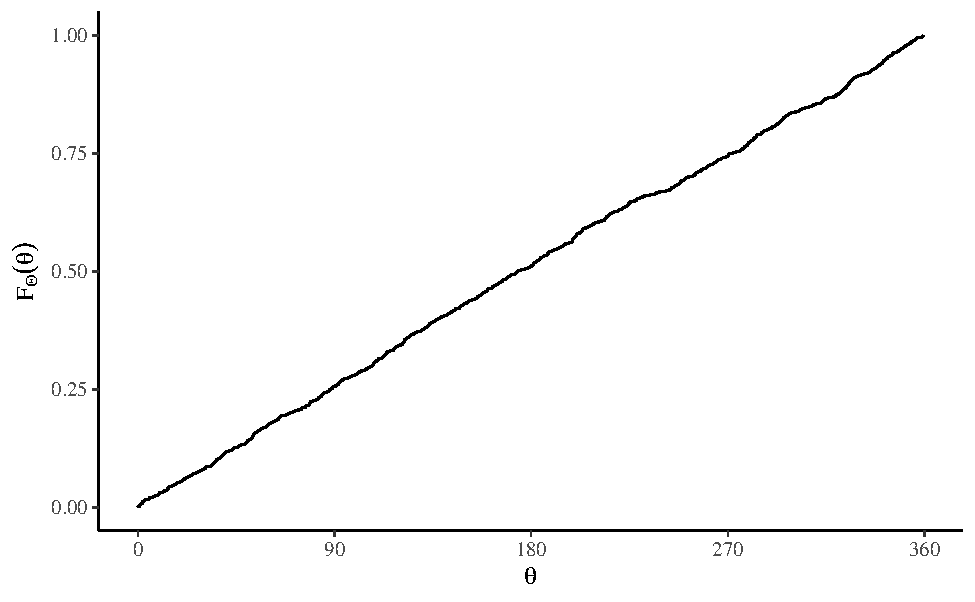
\includegraphics[width=0.95\linewidth]{ds4psy_files/figure-latex/unnamed-chunk-33-1} 

}

\caption{Sulle colonne (a partire da sinistra) i dati utilizzati sono, rispettivamente, (y = 6, n = 13), (y = 29, n = 63) e (y = 66, n = 99). Sulle righe (a partire dall'alto), le distribuzioni a priori usate sono: Beta(14, 1), Beta(5, 11) e Beta(1, 1).}\label{fig:unnamed-chunk-33}
\end{figure}

La figura indica che, se il campione è grande, una distribuzione a priori debolmente informativa ha uno scarso effetto sulla distribuzione a posteriori. Invece, se il campione è piccolo, anche una distribuzione a priori debolmente informativa ha un grande effetto sulla distribuzione a posteriori.

\hypertarget{collegare-le-intuizioni-alla-teoria}{%
\section{Collegare le intuizioni alla teoria}\label{collegare-le-intuizioni-alla-teoria}}

Il compromesso che abbiamo osservato nell'esempio precedente, che combina la distribuzione a priori con le evidenze fornite dai dati, è molto vicino alle nostre intuizioni. Ma è anche il frutto di una necessità matematica. È infatti possibile riscrivere la \eqref{eq:ev-post-beta-bin-1} nel modo seguente

\begin{align}
\E_{\text{post}} &[\text{Beta}(\alpha + y, \beta + n - y)] = \frac{\alpha + y}{\alpha + \beta +n}\notag\\ 
&= \frac{a+b}{a+b+n} \cdot \frac{a}{a+b} + \frac{n}{a+b+n} \cdot \frac{y}{n}.
\label{eq:ev-post-beta-bin}
\end{align}

Ciò indica che il valore atteso a posteriori è una media pesata fra il valore atteso a priori \(\left( \frac{\alpha}{\alpha+\beta}\right)\) e la frequenze di successi osservata \(\left(\frac{y}{n}\right)\). I pesi sono \(\left( \frac{\alpha+\beta}{\alpha+\beta+n}\right)\) e \(\left( \frac{n}{\alpha+\beta+n}\right)\). Quindi, quando \(n\) è grande rispetto ad \(\alpha + \beta\), conta molto quanto abbiamo osservato e conta poco la credenza a priori. Viceversa, quando \(n\) è piccolo rispetto a \(\alpha + \beta\), le osservazioni contano poco rispetto alla credenza a priori.

Queste osservazioni ci fanno capire come scegliere i parametri \(\alpha\) e \(\beta\): se vogliamo assumere una totale ignoranza rispetto al fenomeno in esame, la scelta coerente è \(\alpha = \beta = 1\) (ogni valore di \(\theta\) è ugualmente probabile); se invece abbiamo delle credenze a priori, allora possiamo scegliere \(\alpha\) così che sia uguale al valore atteso a priori, mentre \(\alpha + \beta\) esprime l'importanza che diamo all'informazione a priori: maggiore è il valore di \(\alpha + \beta\), tanti più dati serviranno per allontanare la distribuzione a posteriori dalla distribuzione a priori. Se \(n\) è grande, infine, la distribuzione a posteriori sarà scarsamente influenzata dalla distribuzione a priori, a meno di scelte estreme.

\hypertarget{commenti-e-considerazioni-finali-2}{%
\section*{Commenti e considerazioni finali}\label{commenti-e-considerazioni-finali-2}}


La conclusione che possiamo trarre dall'esempio di \citet{Johnson2022bayesrules} è molto chiara: l'aggiornamento bayesiano può essere paragonato ai processi di ragionamento del senso comune. Quando le nuove evidenze (i dati) sono deboli, non c'è ragione di cambiare idea (le nostre credenze ``a posteriori'' sono molto simili a ciò che pensavamo prima di avere osservato i dati). Quando le nuove evidenze sono irrefutabili, invece, è necessario modificare le nostre credenze sulla base di ciò che ci dicono i dati, quali che siano le nostre credenze pregresse --- non farlo significherebbe vivere in un mondo di fantasia e avere scarse possibilità di sopravvivere nel mondo empirico. L'aggiornamento bayesiano esprime in maniera quantitativa e precisa ciò che ci dicono le nostre intuizioni.

Incredibilmente, però, l'approccio frequentista nega questa logica. I test frequentisti non tengono conto delle conoscenze pregresse. Dunque, se un test frequentista, calcolato su un piccolo campione (ovvero, quando i dati sono molto deboli), suggerisce che dovremmo farci un'opinione di un certo tipo sul fenomeno in esame, l'indicazione è di prendere seriamente il risultato del test \emph{quali siano le evidenze precedenti} --- le quali, possibilmente, mostrano che il risultato del test non ha alcun senso. È sorprendente che un tale modo di pensare possa essere preso sul serio nella comunità scientifica, ma vi sono alcuni ricercatori che continuano a seguire questo modo di (s)ragionare. Dato che in questo Capitolo paliamo di fumetti, concluderei dicendo che la presente discussione è catturata nella maniera più chiara possibile in questa famosa \href{https://xkcd.com/1132/}{striscia}.

\hypertarget{ch:metropolis}{%
\chapter{Approssimazione della distribuzione a posteriori}\label{ch:metropolis}}

In generale, in un problema bayesiano i dati \(y\) provengono da una densità \(p(y \mid \theta)\) e al parametro \(\theta\) viene assegnata una densità a priori \(p(\theta)\). Dopo avere osservato i dati \(Y = y\), la funzione di verosimiglianza è uguale a \(\mathcal{L}(\theta) = p(y \mid \theta)\) e la densità a posteriori diventa

\begin{equation}
p(\theta \mid y) = \frac{p(y \mid \theta) p(\theta)}{\int p(y \mid \theta) p(\theta) \,\operatorname {d}\! \theta}. \notag
\end{equation}

Se vogliamo trovare la distribuzione a posteriori con metodi analitici è necessario ricorrere all'impiego di distribuzioni a priori coniugate, come nello schema beta-binomiale. Per quanto ``semplice'' in termini formali, la scelta di distribuzioni a priori coniugate limita di molto le possibili scelte del ricercatore. Inoltre, non è sempre sensato, dal punto di vista teorico, utilizzare tali distribuzioni per la stima dei parametri di interesse. Il mancato ricorso all'impiego delle distribuzioni a priori coniugate richiede necessariamente il computo dell'espressione a denominatore della formula di Bayes che solo in rare occasioni può essere ottenuta per via analitica. In altre parole, è possibile ottenere analiticamenre la distribuzione a posteriori solo per alcune specifiche combinazioni di distribuzioni a priori e verosimiglianza, il che limita considerevolmente la flessibilità della modellizzazione. Inoltre, i sommari della distribuzione a posteriori sono espressi come rapporto di integrali. Ad esempio, la media a posteriori di \(\theta\) è data da

\begin{equation}
\mathbb{E}(\theta \mid y) = \frac{\int \theta p(y \mid \theta) p(\theta) \,\operatorname {d}\! \theta}{\int p(y \mid \theta) p(\theta) \,\operatorname {d}\! \theta}.\notag
\end{equation}

Il calcolo del valore atteso a posteriori richiede dunque la valutazione di due integrali, ciascuno dei quali non esprimibile in forma chiusa. Per questa ragione, la strada principale che viene seguita nella modellistica bayesiana è quella che porta a determinare la distribuzione a posteriori non per via analitica, ma bensì mediante metodi numerici. La simulazione fornisce dunque la strategia generale del calcolo bayesiano. A questo fine vengono principalmente usati i metodi di campionamento Monte Carlo basati su Catena di Markov (MCMC). Tali metodi costituiscono una potente e praticabile alternativa per la costruzione della distribuzione a posteriori per modelli complessi e consentono di decidere quali distribuzioni a priori e quali distribuzioni di verosimiglianza usare sulla base di considerazioni teoriche soltanto, senza dovere preoccuparsi di altri vincoli.

Dato che è basata su metodi computazionalmente intensivi, la stima numerica della funzione a posteriori può essere svolta soltanto mediante software. In anni recenti i metodi Bayesiani di analisi dei dati sono diventati sempre più popolari proprio perché la potenza di calcolo necessaria per svolgere tali calcoli è ora alla portata di tutti. Questo non era vero solo pochi decenni fa.

In questo Capitolo verranno presentati due metodi di simulazione iterativa\footnote{Si veda anche l'Appendice \ref{appendix:quadratic-approx}.} che consentono di generare dalle distribuzioni a posteriori campioni dei parametri del modello:

\begin{itemize}
\tightlist
\item
  \textbf{metodi basati su griglia:} dove, sebbene non sia disponibile alcuna formula algebrica in forma chiusa, le proprietà della distribuzione a posteriori possono essere calcolate con una precisione arbitraria;
\item
  \textbf{metodi Monte Carlo:} dove, utilizzando appropriate funzioni di numeri casuali, viene generato un ampio campione di casi della variabile casuale per poi stimare empiricamente la proprietà di interesse in base al campione così otttenuto.
\end{itemize}

\hypertarget{metodo-basato-su-griglia}{%
\section{Metodo basato su griglia}\label{metodo-basato-su-griglia}}

Il metodo basato su griglia (\emph{grid-based}) è un metodo numerico esatto basato su una griglia di punti uniformemente spaziati. Anche se la maggior parte dei parametri è continua (ovvero, in linea di principio ciascun parametro può assumere un numero infinito di valori), possiamo ottenere un'eccellente approssimazione della distribuzione a posteriori considerando solo una griglia finita di valori dei parametri. In un tale metodo, la densità di probabilità a posteriori può dunque essere approssimata tramite le densità di probabilità calcolate in ciascuna cella della griglia.

Il metodo basato su griglia si sviluppa in quattro fasi:

\begin{itemize}
\tightlist
\item
  fissare una griglia discreta di possibili valori \(\theta\);
\item
  valutare la distribuzione a priori \(p(\theta)\) e la funzione di verosimiglianza \(p(y \mid \theta)\) in corrispondenza di ciascun valore \(\theta\) della griglia;
\item
  ottenere un'approssimazione discreta della densità a posteriori:

  \begin{itemize}
  \tightlist
  \item
    per ciascun valore \(\theta\) della griglia, calcolare il prodotto \(p(\theta) p(y \mid \theta)\);
  \item
    normalizzare i prodotti così ottenuti in modo tale che la loro somma sia 1;
  \end{itemize}
\item
  selezionare \(N\) valori casuali della griglia in modo tale da ottenere un campione casuale delle densità a posteriori normalizzate.
\end{itemize}

Possiamo migliorare l'approssimazione aumentando il numero di punti della griglia. Infatti utilizzando un numero infinito di punti si otterrebbe la descrizione esatta della distribuzione a posteriori, dovendo però pagare il costo dell'utilizzo di infinite risorse di calcolo. Il limite maggiore dell'approccio basato su griglia è che, al crescere della dimensionalità \(N\) dello spazio dei parametri, i punti della griglia necessari per avere una buona stima crescerebbero esponenzialmente con \(N\), rendendo questo metodo inattuabile.

\hypertarget{modello-beta-binomiale}{%
\subsection{Modello Beta-Binomiale}\label{modello-beta-binomiale}}

Per fare un esempio, consideriamo lo schema beta-binomiale di cui conosciamo la soluzione esatta. Utilizziamo nuovamente i dati di \citet{zetschefuture2019}: 23 ``successi'' in 30 prove Bernoulliane indipendenti.\footnote{Nel presente esempio useremo lo stesso codice \(\R\) utilizzato da \citet{Johnson2022bayesrules}.} Imponiamo alla distribuzione a priori su \(\theta\) (probabilità di successo in una singola prova, laddove per ``successo'' si intende una aspettativa distorta negativamente dell'umore futuro) una \(\mbox{Beta}(2, 10)\) per descrivere la nostra incertezza sul parametro prima di avere osservato i dati. Dunque, il modello diventa:

\begin{align}
Y \mid \theta & \sim \mbox{Bin}(n = 30, \theta), \notag\\
\theta & \sim \mbox{Beta}(2, 10).\notag
\end{align}

In queste circostanze, l'aggiornamento bayesiano produce una distribuzione a posteriori Beta di parametri 25 (\(y + \alpha\) = 23 + 2) e 17 (\(n - y + \beta\) = 30 - 23 + 10):

\begin{equation}
\theta \mid (y = 23) \sim \mbox{Beta}(25, 17).\notag
\end{equation}

Per approssimare la distribuzione a posteriori, fissiamo una griglia di \(n = 11\) valori equispaziati: \(\theta \in \{0, 0.1, 0.2, 0.3, 0.4, 0.5, 0.6, 0.7, 0.8, 0.9, 1\}\):

\begin{Shaded}
\begin{Highlighting}[]
\NormalTok{grid\_data }\OtherTok{\textless{}{-}} \FunctionTok{tibble}\NormalTok{(}
  \AttributeTok{theta\_grid =} \FunctionTok{seq}\NormalTok{(}\AttributeTok{from =} \DecValTok{0}\NormalTok{, }\AttributeTok{to =} \DecValTok{1}\NormalTok{, }\AttributeTok{length.out =} \DecValTok{11}\NormalTok{)}
\NormalTok{)}
\NormalTok{grid\_data}
\CommentTok{\#\textgreater{} \# A tibble: 11 x 1}
\CommentTok{\#\textgreater{}   theta\_grid}
\CommentTok{\#\textgreater{}        \textless{}dbl\textgreater{}}
\CommentTok{\#\textgreater{} 1        0  }
\CommentTok{\#\textgreater{} 2        0.1}
\CommentTok{\#\textgreater{} 3        0.2}
\CommentTok{\#\textgreater{} 4        0.3}
\CommentTok{\#\textgreater{} 5        0.4}
\CommentTok{\#\textgreater{} 6        0.5}
\CommentTok{\#\textgreater{} 7        0.6}
\CommentTok{\#\textgreater{} 8        0.7}
\CommentTok{\#\textgreater{} \# ... with 3 more rows}
\end{Highlighting}
\end{Shaded}

In corrispondenza di ciascun valore della griglia, valutiamo la distribuzione a priori \(\mbox{Beta}(2, 10)\) e la verosimiglianza \(\mbox{Bin}(y = 23, n = 30)\).

\begin{Shaded}
\begin{Highlighting}[]
\NormalTok{grid\_data }\OtherTok{\textless{}{-}}\NormalTok{ grid\_data }\SpecialCharTok{\%\textgreater{}\%}
  \FunctionTok{mutate}\NormalTok{(}
    \AttributeTok{prior =} \FunctionTok{dbeta}\NormalTok{(theta\_grid, }\DecValTok{2}\NormalTok{, }\DecValTok{10}\NormalTok{),}
    \AttributeTok{likelihood =} \FunctionTok{dbinom}\NormalTok{(}\DecValTok{23}\NormalTok{, }\DecValTok{30}\NormalTok{, theta\_grid)}
\NormalTok{  )}
\end{Highlighting}
\end{Shaded}

In ciascuna cella della griglia calcoliamo poi il prodotto della verosimiglianza e della distribuzione a priori. Troviamo così un'approssimazione discreta e non normalizzata della distribuzione a posteriori (\texttt{unnormalized}). Normalizziamo questa approssimazione dividendo ciascun valore \texttt{unnormalized} per la somma di tutti i valori del vettore:

\begin{Shaded}
\begin{Highlighting}[]
\NormalTok{grid\_data }\OtherTok{\textless{}{-}}\NormalTok{ grid\_data }\SpecialCharTok{\%\textgreater{}\%}
  \FunctionTok{mutate}\NormalTok{(}
    \AttributeTok{unnormalized =}\NormalTok{ likelihood }\SpecialCharTok{*}\NormalTok{ prior,}
    \AttributeTok{posterior =}\NormalTok{ unnormalized }\SpecialCharTok{/} \FunctionTok{sum}\NormalTok{(unnormalized)}
\NormalTok{  )}
\end{Highlighting}
\end{Shaded}

Verifichiamo:

\begin{Shaded}
\begin{Highlighting}[]
\NormalTok{grid\_data }\SpecialCharTok{\%\textgreater{}\%}
  \FunctionTok{summarize}\NormalTok{(}
    \FunctionTok{sum}\NormalTok{(unnormalized),}
    \FunctionTok{sum}\NormalTok{(posterior)}
\NormalTok{  )}
\CommentTok{\#\textgreater{} \# A tibble: 1 x 2}
\CommentTok{\#\textgreater{}   \textasciigrave{}sum(unnormalized)\textasciigrave{} \textasciigrave{}sum(posterior)\textasciigrave{}}
\CommentTok{\#\textgreater{}                 \textless{}dbl\textgreater{}            \textless{}dbl\textgreater{}}
\CommentTok{\#\textgreater{} 1            0.000869                1}
\end{Highlighting}
\end{Shaded}

Abbiamo dunque ottenuto la seguente distribuzione a posteriori discretizzata \(p(\theta \mid y)\):

\begin{Shaded}
\begin{Highlighting}[]
\FunctionTok{round}\NormalTok{(grid\_data, }\DecValTok{2}\NormalTok{)}
\CommentTok{\#\textgreater{} \# A tibble: 11 x 5}
\CommentTok{\#\textgreater{}   theta\_grid prior likelihood unnormalized posterior}
\CommentTok{\#\textgreater{}        \textless{}dbl\textgreater{} \textless{}dbl\textgreater{}      \textless{}dbl\textgreater{}        \textless{}dbl\textgreater{}     \textless{}dbl\textgreater{}}
\CommentTok{\#\textgreater{} 1        0    0          0               0      0   }
\CommentTok{\#\textgreater{} 2        0.1  4.26       0               0      0   }
\CommentTok{\#\textgreater{} 3        0.2  2.95       0               0      0   }
\CommentTok{\#\textgreater{} 4        0.3  1.33       0               0      0   }
\CommentTok{\#\textgreater{} 5        0.4  0.44       0               0      0.02}
\CommentTok{\#\textgreater{} 6        0.5  0.11       0               0      0.23}
\CommentTok{\#\textgreater{} 7        0.6  0.02       0.03            0      0.52}
\CommentTok{\#\textgreater{} 8        0.7  0          0.12            0      0.21}
\CommentTok{\#\textgreater{} \# ... with 3 more rows}
\end{Highlighting}
\end{Shaded}

La figura \ref{fig:grid-method-6points-posterior-plot} mostra un grafico della distribuzione a posteriori discretizzata così ottenuta:

\begin{Shaded}
\begin{Highlighting}[]
\NormalTok{grid\_data }\SpecialCharTok{\%\textgreater{}\%} 
  \FunctionTok{ggplot}\NormalTok{(}
    \FunctionTok{aes}\NormalTok{(}\AttributeTok{x =}\NormalTok{ theta\_grid, }\AttributeTok{y =}\NormalTok{ posterior)}
\NormalTok{  ) }\SpecialCharTok{+}
  \FunctionTok{geom\_point}\NormalTok{() }\SpecialCharTok{+}
  \FunctionTok{geom\_segment}\NormalTok{(}
    \FunctionTok{aes}\NormalTok{(}
      \AttributeTok{x =}\NormalTok{ theta\_grid, }
      \AttributeTok{xend =}\NormalTok{ theta\_grid, }
      \AttributeTok{y =} \DecValTok{0}\NormalTok{, }
      \AttributeTok{yend =}\NormalTok{ posterior)}
\NormalTok{  )}
\end{Highlighting}
\end{Shaded}

\begin{figure}[h]

{\centering 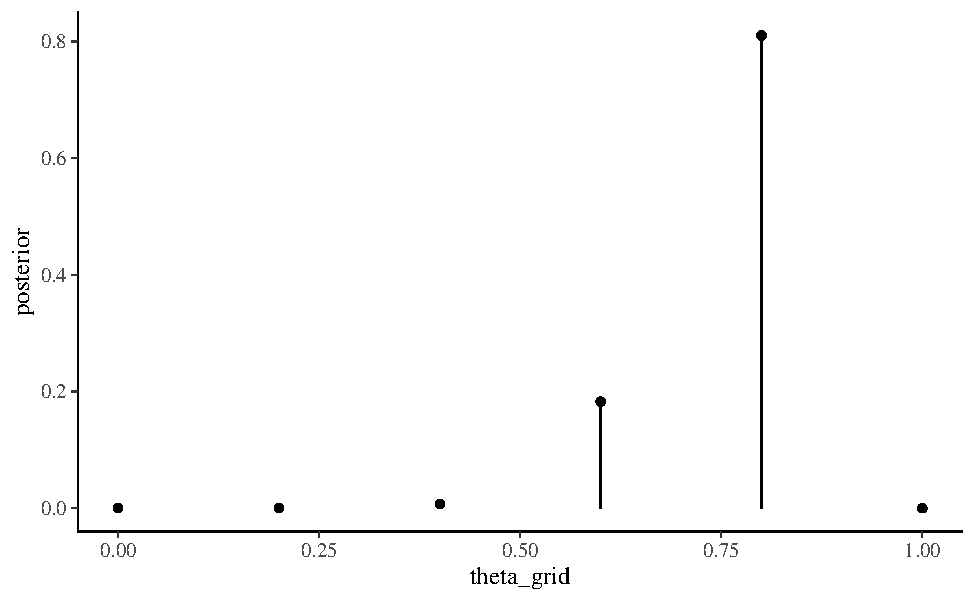
\includegraphics{ds4psy_files/figure-latex/grid-method-6points-posterior-plot-1} 

}

\caption{Distribuzione a posteriori discretizzata ottenuta con il metodo grid-based per $y$ = 23 successi in 30 prove Bernoulliane, con distribuzione a priori $\mbox{Beta}(2, 10)$. È stata utilizzata una griglia di solo $n$ = 11 punti.}\label{fig:grid-method-6points-posterior-plot}
\end{figure}

L'ultimo passo della simulazione è il campionamento dalla distribuzione a posteriori discretizzata:

\begin{Shaded}
\begin{Highlighting}[]
\FunctionTok{set.seed}\NormalTok{(}\DecValTok{84735}\NormalTok{)}
\NormalTok{post\_sample }\OtherTok{\textless{}{-}} \FunctionTok{sample\_n}\NormalTok{(}
\NormalTok{  grid\_data,}
  \AttributeTok{size =} \FloatTok{1e5}\NormalTok{,}
  \AttributeTok{weight =}\NormalTok{ posterior,}
  \AttributeTok{replace =} \ConstantTok{TRUE}
\NormalTok{)}
\end{Highlighting}
\end{Shaded}

La figura \ref{fig:grid-method-6points-posterior-plot-sampling} mostra che, con una griglia così sparsa abbiamo ottenuto una versione approssimata della vera distribuzione a posteriori (all'istogramma è stata sovrapposta l'esatta distribuzione a posteriori \(\mbox{Beta}(25, 17)\)).

\begin{Shaded}
\begin{Highlighting}[]
\FunctionTok{ggplot}\NormalTok{(post\_sample, }\FunctionTok{aes}\NormalTok{(}\AttributeTok{x =}\NormalTok{ theta\_grid)) }\SpecialCharTok{+}
  \FunctionTok{geom\_histogram}\NormalTok{(}\FunctionTok{aes}\NormalTok{(}\AttributeTok{y =}\NormalTok{ ..density..), }\AttributeTok{color =} \StringTok{"white"}\NormalTok{) }\SpecialCharTok{+}
  \FunctionTok{stat\_function}\NormalTok{(}\AttributeTok{fun =}\NormalTok{ dbeta, }\AttributeTok{args =} \FunctionTok{list}\NormalTok{(}\DecValTok{25}\NormalTok{, }\DecValTok{17}\NormalTok{)) }\SpecialCharTok{+}
  \FunctionTok{lims}\NormalTok{(}\AttributeTok{x =} \FunctionTok{c}\NormalTok{(}\DecValTok{0}\NormalTok{, }\DecValTok{1}\NormalTok{))}
\end{Highlighting}
\end{Shaded}

\begin{figure}[h]

{\centering 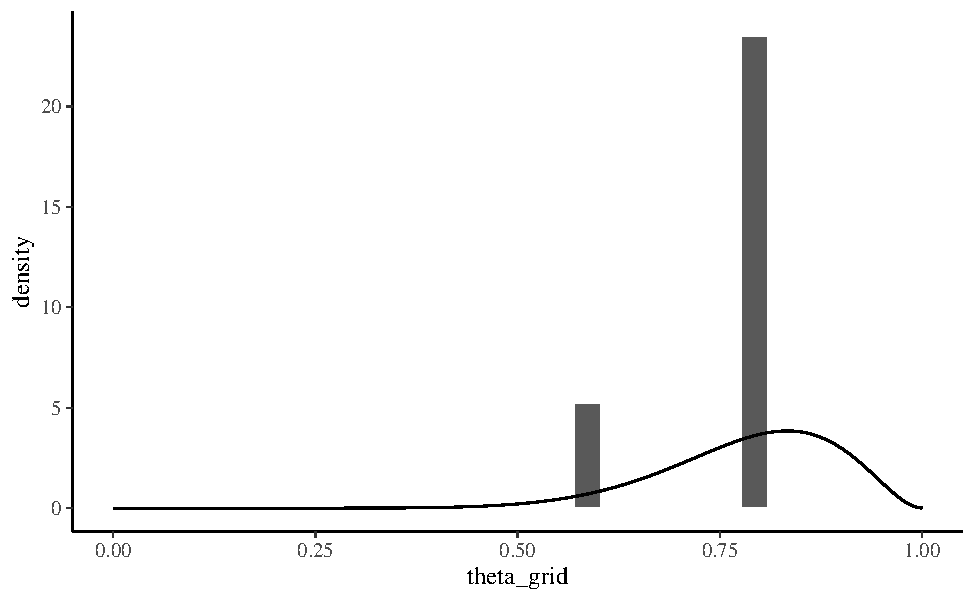
\includegraphics{ds4psy_files/figure-latex/grid-method-6points-posterior-plot-sampling-1} 

}

\caption{Campionamento dalla  distribuzione a posteriori discretizzata ottenuta con il metodo grid-based per $y$ = 23 successi in 30 prove Bernoulliane, con distribuzione a priori $\mbox{Beta}(2, 10)$. È stata utilizzata una griglia di solo $n$ = 11 punti.}\label{fig:grid-method-6points-posterior-plot-sampling}
\end{figure}

Possiamo ottenere un risultato migliore con una griglia più fine, come indicato nella figura \ref{fig:grid-method-100points-posterior-plot-sampling}:

\begin{Shaded}
\begin{Highlighting}[]
\NormalTok{grid\_data }\OtherTok{\textless{}{-}} \FunctionTok{tibble}\NormalTok{(}
  \AttributeTok{theta\_grid =} \FunctionTok{seq}\NormalTok{(}\AttributeTok{from =} \DecValTok{0}\NormalTok{, }\AttributeTok{to =} \DecValTok{1}\NormalTok{, }\AttributeTok{length.out =} \DecValTok{100}\NormalTok{)}
\NormalTok{)}
\NormalTok{grid\_data }\OtherTok{\textless{}{-}}\NormalTok{ grid\_data }\SpecialCharTok{\%\textgreater{}\%}
  \FunctionTok{mutate}\NormalTok{(}
    \AttributeTok{prior =} \FunctionTok{dbeta}\NormalTok{(theta\_grid, }\DecValTok{2}\NormalTok{, }\DecValTok{10}\NormalTok{),}
    \AttributeTok{likelihood =} \FunctionTok{dbinom}\NormalTok{(}\DecValTok{23}\NormalTok{, }\DecValTok{30}\NormalTok{, theta\_grid)}
\NormalTok{  )}
\NormalTok{grid\_data }\OtherTok{\textless{}{-}}\NormalTok{ grid\_data }\SpecialCharTok{\%\textgreater{}\%}
  \FunctionTok{mutate}\NormalTok{(}
    \AttributeTok{unnormalized =}\NormalTok{ likelihood }\SpecialCharTok{*}\NormalTok{ prior,}
    \AttributeTok{posterior =}\NormalTok{ unnormalized }\SpecialCharTok{/} \FunctionTok{sum}\NormalTok{(unnormalized)}
\NormalTok{  )}
\NormalTok{grid\_data }\SpecialCharTok{\%\textgreater{}\%}
  \FunctionTok{ggplot}\NormalTok{(}
    \FunctionTok{aes}\NormalTok{(}\AttributeTok{x =}\NormalTok{ theta\_grid, }\AttributeTok{y =}\NormalTok{ posterior)}
\NormalTok{  ) }\SpecialCharTok{+}
  \FunctionTok{geom\_point}\NormalTok{() }\SpecialCharTok{+}
  \FunctionTok{geom\_segment}\NormalTok{(}
    \FunctionTok{aes}\NormalTok{(}
      \AttributeTok{x =}\NormalTok{ theta\_grid,}
      \AttributeTok{xend =}\NormalTok{ theta\_grid,}
      \AttributeTok{y =} \DecValTok{0}\NormalTok{,}
      \AttributeTok{yend =}\NormalTok{ posterior}
\NormalTok{    )}
\NormalTok{  )}
\end{Highlighting}
\end{Shaded}

\begin{figure}[h]

{\centering 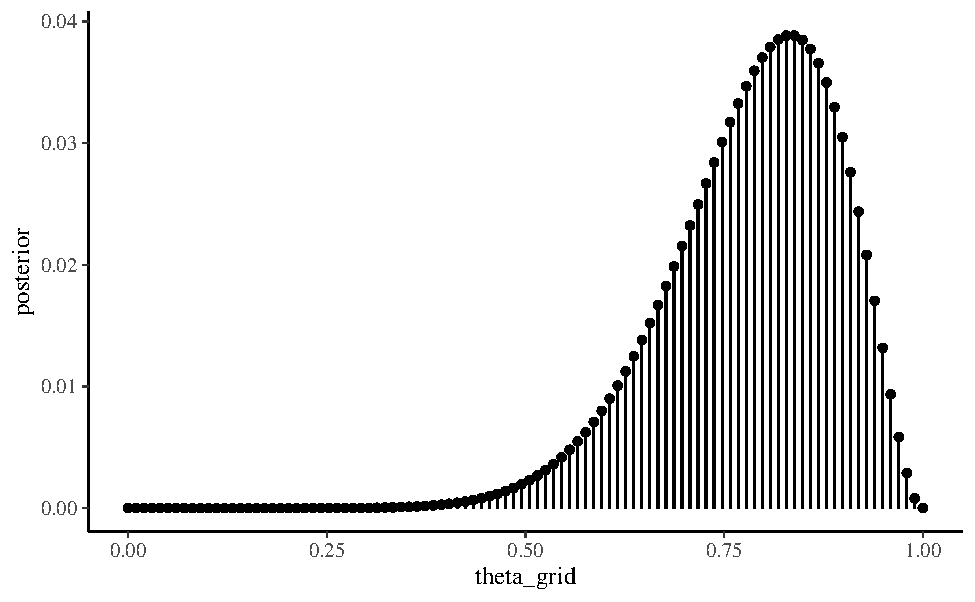
\includegraphics{ds4psy_files/figure-latex/grid-method-100points-posterior-plot-sampling-1} 

}

\caption{Distribuzione a posteriori discretizzata ottenuta con il metodo grid-based per $y$ = 23 successi in 30 prove Bernoulliane, con distribuzione a priori $\mbox{Beta}(2, 10)$. È stata utilizzata una griglia di $n$ = 100 punti.}\label{fig:grid-method-100points-posterior-plot-sampling}
\end{figure}

Campioniamo ora 10000 punti:

\begin{Shaded}
\begin{Highlighting}[]
\CommentTok{\# Set the seed}
\FunctionTok{set.seed}\NormalTok{(}\DecValTok{84735}\NormalTok{)}
\NormalTok{post\_sample }\OtherTok{\textless{}{-}} \FunctionTok{sample\_n}\NormalTok{(}
\NormalTok{  grid\_data,}
  \AttributeTok{size =} \FloatTok{1e4}\NormalTok{,}
  \AttributeTok{weight =}\NormalTok{ posterior,}
  \AttributeTok{replace =} \ConstantTok{TRUE}
\NormalTok{)}
\end{Highlighting}
\end{Shaded}

Con il campionamento dalla distribuzione a posteriori discretizzata costruita mediante una griglia più densa (\(n = 100\)) otteniamo un risultato soddisfacente (figura \ref{fig:grid-method-100points-posterior-plot-and-correct-posterior}): ora la distribuzione dei valori prodotti dalla simulazione approssima molto bene la corretta distribuzione a posteriori \(p(\theta \mid y) = \mbox{Beta}(25, 17)\).

\begin{Shaded}
\begin{Highlighting}[]
\NormalTok{post\_sample }\SpecialCharTok{\%\textgreater{}\%}
  \FunctionTok{ggplot}\NormalTok{(}\FunctionTok{aes}\NormalTok{(}\AttributeTok{x =}\NormalTok{ theta\_grid)) }\SpecialCharTok{+}
  \FunctionTok{geom\_histogram}\NormalTok{(}
    \FunctionTok{aes}\NormalTok{(}\AttributeTok{y =}\NormalTok{ ..density..),}
    \AttributeTok{color =} \StringTok{"white"}\NormalTok{,}
    \AttributeTok{bins=}\DecValTok{50}
\NormalTok{  ) }\SpecialCharTok{+}
  \FunctionTok{stat\_function}\NormalTok{(}\AttributeTok{fun =}\NormalTok{ dbeta, }\AttributeTok{args =} \FunctionTok{list}\NormalTok{(}\DecValTok{25}\NormalTok{, }\DecValTok{17}\NormalTok{)) }\SpecialCharTok{+}
  \FunctionTok{lims}\NormalTok{(}\AttributeTok{x =} \FunctionTok{c}\NormalTok{(}\DecValTok{0}\NormalTok{, }\DecValTok{1}\NormalTok{))}
\end{Highlighting}
\end{Shaded}

\begin{figure}[h]

{\centering 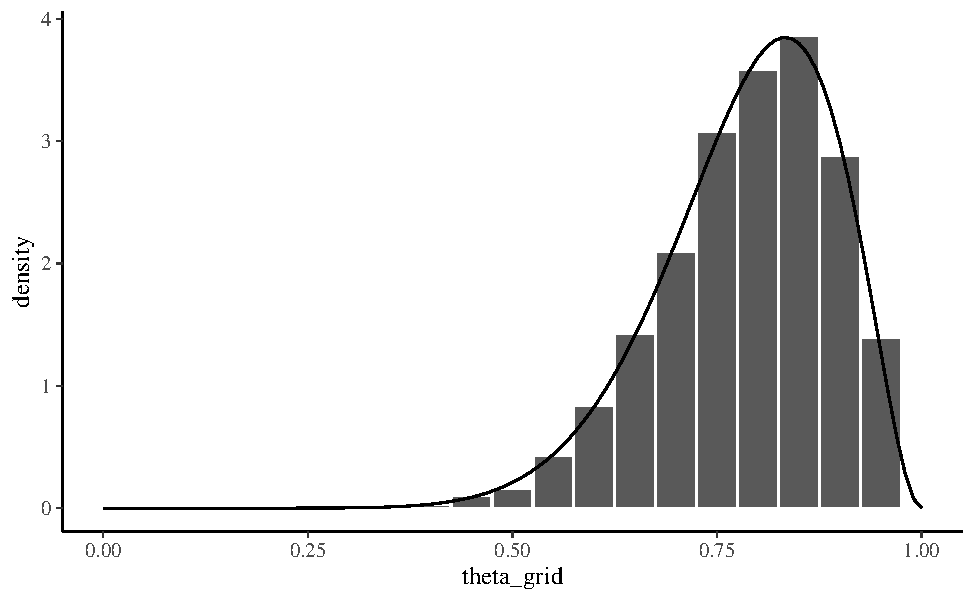
\includegraphics{ds4psy_files/figure-latex/grid-method-100points-posterior-plot-and-correct-posterior-1} 

}

\caption{Campionamento dalla  distribuzione a posteriori discretizzata ottenuta con il metodo grid-based per $y$ = 23 successi in 30 prove Bernoulliane, con distribuzione a priori $\mbox{Beta}(2, 10)$. È stata utilizzata una griglia di $n$ = 100 punti. All'istogramma è stata sovrapposta la corretta distribuzione a posteriori, ovvero la densità $\mbox{Beta}(25, 17)$.}\label{fig:grid-method-100points-posterior-plot-and-correct-posterior}
\end{figure}

In conclusione, il metodo basato su griglia è molto intuitivo e non richiede particolari competenze di programmazione per essere implementato. Inoltre, fornisce un risultato che, per tutti gli scopi pratici, può essere considerato come un campione casuale estratto da \(p(\theta \mid y)\). Tuttavia, anche se tale metodo fornisce risultati accuratissimi, esso ha un uso limitato. A causa della \emph{maledizione della dimensionalità}\footnote{Per capire cosa sia la maledizione della dimensionalità, supponiamo di utilizzare una griglia di 100 punti equispaziati. Nel caso di un solo parametro, è necessario calcolare 100 valori. Per due parametri devono essere calcolari \(100^2\) valori. Ma già per 10 parametri è necessario calcolare \(10^{10}\) valori -- è facile capire che una tale quantità di calcoli è troppo grande anche per un computer molto potente. Per modelli che richiedono la stima di un numero non piccolo di parametri è dunque necessario procedere in un altro modo.}, tale metodo può solo essere solo nel caso di semplici modelli statistici, con non più di due parametri. Nella pratica concreta tale metodo viene dunque sostituito da altre tecniche più efficienti in quanto, anche nei più comuni modelli utilizzati in psicologia, vengono solitamente stimati centinaia se non migliaia di parametri.

\hypertarget{chapter-simulazioneMC}{%
\section{Metodo Monte Carlo}\label{chapter-simulazioneMC}}

I metodi più ampiamente adottati nell'analisi bayesiana per la costruzione della distribuzione a posteriori per modelli complessi sono i metodi di campionamento MCMC. Tali metodi consentono al ricercatore di decidere quali distribuzioni a priori e quali distribuzioni di verosimiglianza usare sulla base di considerazioni teoriche soltanto, senza doversi preoccupare di altri vincoli. Dato che è basata su metodi computazionalmente intensivi, la stima numerica MCMC della funzione a posteriori può essere svolta soltanto mediante software. In anni recenti i metodi Bayesiani di analisi dei dati sono diventati sempre più popolari proprio perché la potenza di calcolo necessaria per svolgere tali calcoli è alla portata di tutti. Questo non era vero solo pochi decenni fa.

\hypertarget{integration-mc}{%
\subsection{Integrazione di Monte Carlo}\label{integration-mc}}

Il termine Monte Carlo si riferisce al fatto che la computazione fa ricorso ad un ripetuto campionamento casuale attraverso la generazione di sequenze di numeri casuali. Una delle sue applicazioni più potenti è il calcolo degli integrali mediante simulazione numerica. Data una successione di realizzazioni indipendenti \(y^{(1)}, y^{(2)},\dots, y^{(T)}\) da una distribuzione \(p(y)\) con media \(\mu\) abbiamo che

\[
\E(Y) = \int y p(y) \,\operatorname {d}\!y \approx \frac{1}{T} \sum_{i=1}^T y^{(t)}.
\]

In altre parole, l'aspettazione teorica di \(Y\) può essere approssimata dalla media campionaria di un insieme di realizzazioni indipendenti ricavate da \(p(y)\). Per la Legge Forte dei Grandi Numeri, l'approssimazione diventa arbitrariamente esatta per \(T \rightarrow \infty\). L'integrazione Monte Carlo può essere utilizzata anche per la valutazione di integrali più complessi.

Quello che è stato detto sopra non è altro che un modo sofisticato per dire che, se vogliamo calcolare un'approssimazione del valore atteso di una variabile casuale, non dobbiamo fare altro che la media aritmetica di un grande numero di realizzazioni indipendenti della variabile casuale. Come è facile intuire, l'approssimazione migliora al crescere del numero di dati che abbiamo a disposizione.

Un'altra importante funzione di \(Y\) è la funzione indicatore, \(I(l < Y < u)\), che assume valore 1 se \(Y\) giace nell'intervallo \((l,u)\) e 0 altrimenti. Il valore di aspettazione di \(I(l < X < u)\) rispetto a \(p(x)\) dà la probabilità che \(Y\) rientri nell'intervallo specificato, \(Pr(l < T < u)\), e può essere approssimato usando l'integrazione Monte Carlo, ovvero prendendo la media campionaria del valore della funzione indicatore per ogni realizzazione \(y^{(t)}\). È semplice vedere come

\[
Pr(l < Y < u) \approx \frac{\text{numero di realizzazioni } y^{(t)} \in (l, u)}{T}.
\]

Presentiamo qui l'integrazione di Monte Carlo perché può essere usata per approssimare la distribuzione a posteriori richiesta da un'analisi Bayesiana: una stima di \(p(\theta \mid y)\) viene infatti ottenuta mediante un grande numero di campioni casuali estratti dalla distribuzionea a posteriori.

\hypertarget{un-esempio-concreto-3}{%
\subsection{Un esempio concreto}\label{un-esempio-concreto-3}}

Per introdurre i metodi MCMC consideriamo nuovamente i dati di \citet{zetschefuture2019} (23 ``successi'' in 30 prove Bernoulliane) che possono essere analizzati mediante lo schema beta-binomiale. In questo caso, la distribuzione a posteriori può essere ottenuta analiticamente ed è uguale ad una \(\mbox{Beta}(25, 17)\). Se vogliamo trovare il valore della media a posteriori di \(\theta\), il risultato esatto è

\[
\bar{\theta}_{post} = \frac{\alpha}{\alpha + \beta} = \frac{25}{25 + 17} \approx 0.5952.
\]

In alternativa, sapendo che la distribuzione a posteriori di \(\theta\) è \(\mbox{Beta}(25, 17)\), possiamo estrarre un campione casuale di osservazioni da tale distribuzione e calcolare la media. Con solo 10 osservazioni otteniamo:

\begin{Shaded}
\begin{Highlighting}[]
\FunctionTok{set.seed}\NormalTok{(}\DecValTok{84735}\NormalTok{)}
\FunctionTok{print}\NormalTok{(}\FunctionTok{mean}\NormalTok{(}\FunctionTok{rbeta}\NormalTok{(}\FloatTok{1e2}\NormalTok{, }\AttributeTok{shape1 =} \DecValTok{25}\NormalTok{, }\AttributeTok{shape2 =} \DecValTok{17}\NormalTok{)), }\DecValTok{6}\NormalTok{)}
\CommentTok{\#\textgreater{} [1] 0.584251}
\end{Highlighting}
\end{Shaded}

L'approssimazione migliora all'aumentare del numero di osservazioni (legge dei grandi numeri):

\begin{Shaded}
\begin{Highlighting}[]
\FunctionTok{print}\NormalTok{(}\FunctionTok{mean}\NormalTok{(}\FunctionTok{rbeta}\NormalTok{(}\FloatTok{1e4}\NormalTok{, }\AttributeTok{shape1 =} \DecValTok{25}\NormalTok{, }\AttributeTok{shape2 =} \DecValTok{17}\NormalTok{)), }\DecValTok{6}\NormalTok{)}
\CommentTok{\#\textgreater{} [1] 0.595492}
\FunctionTok{print}\NormalTok{(}\FunctionTok{mean}\NormalTok{(}\FunctionTok{rbeta}\NormalTok{(}\FloatTok{1e6}\NormalTok{, }\AttributeTok{shape1 =} \DecValTok{25}\NormalTok{, }\AttributeTok{shape2 =} \DecValTok{17}\NormalTok{)), }\DecValTok{6}\NormalTok{)}
\CommentTok{\#\textgreater{} [1] 0.595192}
\end{Highlighting}
\end{Shaded}

Quando il numero di osservazioni (possiamo anche chiamarle ``campioni'') tratte dalla distribuzione a posteriori è molto grande, la distribuzione di tali campioni converge alla densità della popolazione (si veda l'Appendice \ref{integration-mc}).\footnote{Si noti che il numero dei campioni di simulazione è controllato dal ricercatore; tale valore è totalmente diverso dalla dimensione del campione che è fissa ed è una proprietà dei dati.}

Le statistiche descrittive (media, moda, varianza, eccetera) dei campioni estratti dalla distribuzione a posteriori convergeranno ai corrispondenti valori della distribuzione a posteriori. La figura \ref{fig:mcmc-chains-1} mostra come, all'aumentare del numero di repliche, la media, la mediana, la deviazione standard e l'asimmetria convergono ai veri valori della distribuzione a posteriori (linee rosse tratteggiate).

\begin{figure}[h]

{\centering 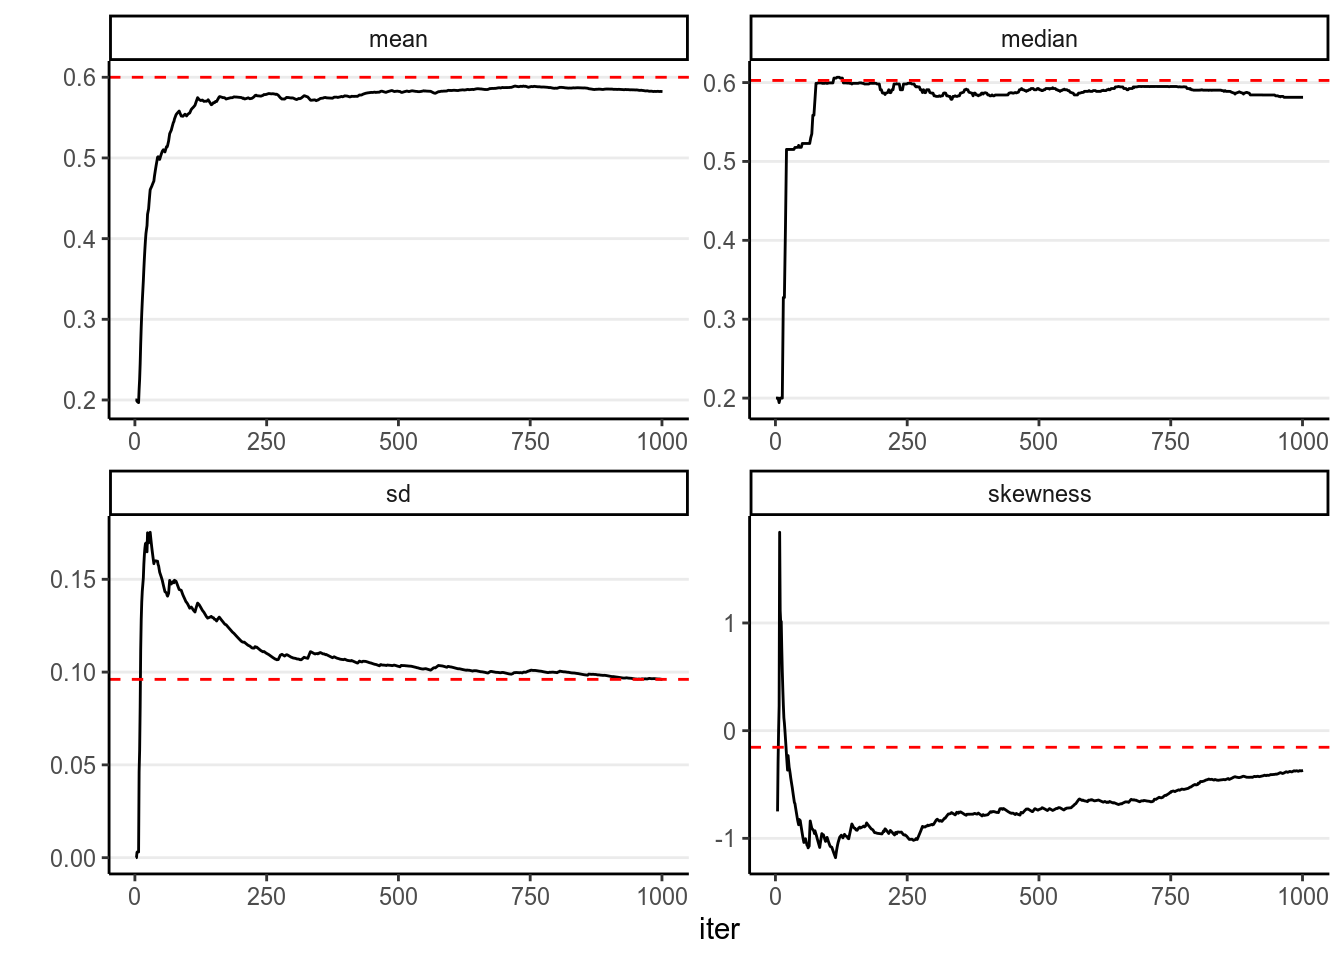
\includegraphics[width=0.8\linewidth]{/Users/corrado/_repositories/ds4psy/images/mcmc-chains-1} 

}

\caption{Convergenza delle simulazioni Monte Carlo.}\label{fig:mcmc-chains-1}
\end{figure}

\hypertarget{metodi-mc-basati-su-catena-di-markov}{%
\subsection{Metodi MC basati su Catena di Markov}\label{metodi-mc-basati-su-catena-di-markov}}

Nel Paragrafo \ref{chapter-simulazioneMC} la simulazione Monte Carlo produceva il risultato desiderato perché

\begin{itemize}
\tightlist
\item
  sapevamo che la distribuzione a posteriori era una \(\mbox{Beta}(25, 17)\),
\item
  era possibile usare le funzioni \(\R\) per estrarre campioni casuali da tale distribuzione.
\end{itemize}

Tuttavia, capita raramente di usare una distribuzione a priori coniugata alla verosimiglianza. Quindi, in generale, le due condizioni descritte sopra non si applicano. Ad esempio, nel caso di una verosimiglianza binomiale e di una distribuzione a priori gaussiana, la distribuzione a posteriori di \(\theta\) è

\[
p(\theta \mid y) = \frac{\mathrm{e}^{-(\theta - 1 / 2)^2} \theta^y (1 - \theta)^{n - y}} {\int_0^1 \mathrm{e}^{-(t - 1 / 2)^2} t^y (1 - t)^{n - y} dt}.
\]

Una tale distribuzione non è implementata in \(\R\) e dunque non possiamo campionare da essa.

Il vantaggio degli algoritmi MCMC è che essi consentono il campionamento da una distribuzione a posteriori \emph{senza che sia necessario conoscere la rappresentazione analitica di una tale distribuzione}.

I metodi MCMC consentono di costruire sequenze di punti (detti catene di Markov) nello spazio dei parametri le cui densità sono proporzionali alla distribuzione a posteriori --- in altre parole, dopo aver simulato un grande numero di passi della catena si possono usare i valori così generati come se fossero un campione casuale della distribuzione a posteriori. Le tecniche MCMC sono attualmente il metodo computazionale maggiormente usato per risolvere i problemi dell'inferenza bayesiana. Un'introduzione alle catene di Markov è fornita nell'Appendice \ref{markov-chains}.

\hypertarget{campionamento-mediante-algoritmi-mcmc}{%
\subsection{Campionamento mediante algoritmi MCMC}\label{campionamento-mediante-algoritmi-mcmc}}

Il metodo (computazionalmente) più semplice per ottenere una catena di Markov la cui distribuzione equivale alla distribuzione a posteriori \(p(\theta \mid y)\) è quello di usare l'algoritmo di Metropolis. L'algoritmo di Metropolis è il primo algoritmo MCMC che è stato proposto ed è applicabile ad una grande varietà di problemi inferenziali di tipo bayesiano. Questo algoritmo è stato in seguito sviluppato allo scopo di renderlo via via più efficente.

\hypertarget{una-passeggiata-casuale-sui-numeri-naturali}{%
\subsection{Una passeggiata casuale sui numeri naturali}\label{una-passeggiata-casuale-sui-numeri-naturali}}

Per introdurre l'algoritmo di di Metropolis in una forma intuitiva consideriamo ora il campionamento da una distribuzione discreta.\footnote{Seguiamo qui la trattazione di \citet{albert2019probability}. Per una presentazione dell'idea che sta alla base dell'algoritmo di Metropolis, si vedano anche \citet{doing_bayesian_data_an}; \citet{McElreath_rethinking}.} Supponiamo di definire una distribuzione di probabilità discreta sugli interi \(1,\dots, K\). Scriviamo in \(\R\) la funzione \texttt{pd()} che assegna ai valori \(1,\dots, 8\) valori di probabilità proporzionali a 5, 10, 4, 4, 20, 20, 12 e 5.

\begin{Shaded}
\begin{Highlighting}[]
\NormalTok{pd }\OtherTok{\textless{}{-}} \ControlFlowTok{function}\NormalTok{(x)\{}
\NormalTok{  values }\OtherTok{\textless{}{-}} \FunctionTok{c}\NormalTok{(}\DecValTok{5}\NormalTok{, }\DecValTok{10}\NormalTok{, }\DecValTok{4}\NormalTok{, }\DecValTok{4}\NormalTok{, }\DecValTok{20}\NormalTok{, }\DecValTok{20}\NormalTok{, }\DecValTok{12}\NormalTok{, }\DecValTok{5}\NormalTok{)}
  \FunctionTok{ifelse}\NormalTok{(}
\NormalTok{    x }\SpecialCharTok{\%in\%} \DecValTok{1}\SpecialCharTok{:}\FunctionTok{length}\NormalTok{(values),}
\NormalTok{    values[x] }\SpecialCharTok{/} \FunctionTok{sum}\NormalTok{(values),}
    \DecValTok{0}
\NormalTok{  )}
\NormalTok{\}}
\NormalTok{prob\_dist }\OtherTok{\textless{}{-}} \FunctionTok{tibble}\NormalTok{(}
  \AttributeTok{x =} \DecValTok{1}\SpecialCharTok{:}\DecValTok{8}\NormalTok{,}
  \AttributeTok{prob =} \FunctionTok{pd}\NormalTok{(}\DecValTok{1}\SpecialCharTok{:}\DecValTok{8}\NormalTok{)}
\NormalTok{)}
\end{Highlighting}
\end{Shaded}

La figura \ref{fig:formetropolisdistr} illustra la distribuzione di probabilità che è stata generata in questo modo.

\begin{Shaded}
\begin{Highlighting}[]
\NormalTok{x }\OtherTok{\textless{}{-}} \DecValTok{1}\SpecialCharTok{:}\DecValTok{8}
\NormalTok{prob\_dist }\SpecialCharTok{\%\textgreater{}\%}
  \FunctionTok{ggplot}\NormalTok{(}\FunctionTok{aes}\NormalTok{(}\AttributeTok{x =}\NormalTok{ x, }\AttributeTok{y =}\NormalTok{ prob)) }\SpecialCharTok{+}
  \FunctionTok{geom\_bar}\NormalTok{(}\AttributeTok{stat =} \StringTok{"identity"}\NormalTok{, }\AttributeTok{width =} \FloatTok{0.06}\NormalTok{) }\SpecialCharTok{+}
  \FunctionTok{scale\_x\_continuous}\NormalTok{(}\StringTok{"x"}\NormalTok{, }\AttributeTok{labels =} \FunctionTok{as.character}\NormalTok{(x), }\AttributeTok{breaks =}\NormalTok{ x) }\SpecialCharTok{+}
  \FunctionTok{labs}\NormalTok{(}
    \AttributeTok{y =} \StringTok{"Probabilità"}\NormalTok{,}
    \AttributeTok{x =} \StringTok{"X"}
\NormalTok{  )}
\end{Highlighting}
\end{Shaded}

\begin{figure}[h]

{\centering 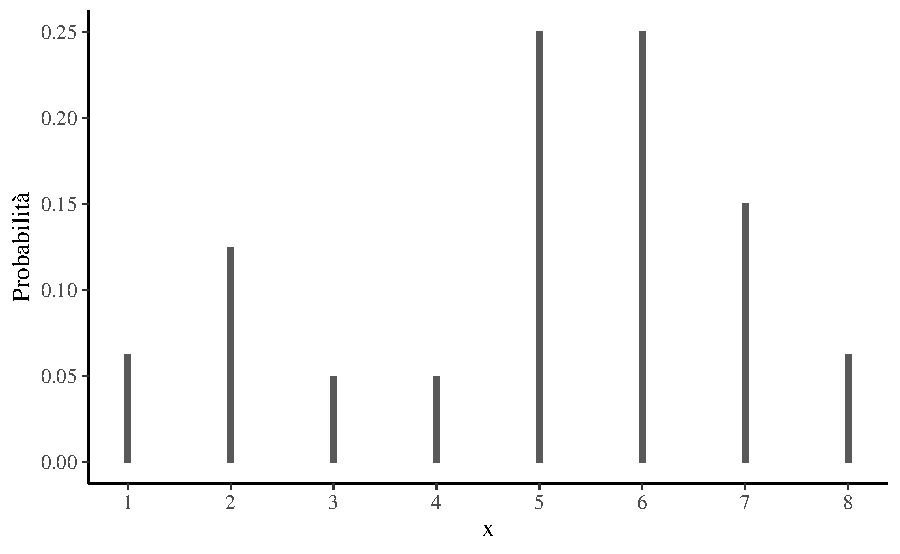
\includegraphics{ds4psy_files/figure-latex/formetropolisdistr-1} 

}

\caption{Distribuzione di massa di probabilità della variabile casuale discreta $X$ avente supporto $\{1, 2, ..., 8\}$.}\label{fig:formetropolisdistr}
\end{figure}

L'algoritmo di Metropolis corrisponde alla seguente passeggiata casuale.

\begin{enumerate}
\def\labelenumi{\arabic{enumi}.}
\tightlist
\item
  L'algoritmo inizia con un valore iniziale qualsiasi da 1 a \(K=8\) della variabile casuale.
\item
  Per simulare il valore successivo della sequenza, lanciamo una moneta equilibrata. Se esce testa, consideriamo come valore candidato il valore immediatamente precedente al valore corrente nella sequenza \(1, \dots, 8\); se esce croce, il candidato è il valore immediatamente successivo a quello corrente nella sequenza.
\item
  Si calcola il rapporto \(R\) tra la probabilità del valore candidato e la probabilità del valore corrente:
\end{enumerate}

\[
R = \frac{pd(\text{valore candidato})}{pd(\text{valore corrente})}.
\]

\begin{enumerate}
\def\labelenumi{\arabic{enumi}.}
\setcounter{enumi}{3}
\tightlist
\item
  Si estrae un numero a caso \(\in [0, 1]\). Se tale valore è minore di \(R\) si accetta il valore candidato come valore successivo della catena markoviana; altrimenti il valore successivo della catena rimane il valore corrente.
\end{enumerate}

In termini tecnici (si veda l'Appendice \ref{markov-chains}), i passi da 1 a 4 definiscono una catena di Markov irriducibile e aperiodica sui valori di stato \(\{1, 2,\dots, 8\}\), dove il passo 1 fornisce il valore iniziale della catena e i passi da 2 a 4 definiscono la matrice di transizione \(P\). Il campionamento dalla distribuzione di massa \texttt{pd} corrisponde ad una passeggiata casuale, che inizia da una posizione qualsiasi, e che ripete le fasi 2, 3 e 4 dell'algoritmo di Metropolis. Dopo un grande numero di passi, la distribuzione dei valori della catena markoviana approssimerà la distribuzione di probabilità \texttt{pd}.

La seguente funzione \texttt{random\_walk()} implementa l'algoritmo di Metropolis. Tale funzione prende in input la distribuzione di probabilità \texttt{pd}, la posizione di partenza \texttt{start} e il numero di passi dell'algoritmo \texttt{num\_steps}.

\begin{Shaded}
\begin{Highlighting}[]
\NormalTok{random\_walk }\OtherTok{\textless{}{-}} \ControlFlowTok{function}\NormalTok{(pd, start, num\_steps)\{}
\NormalTok{  y }\OtherTok{\textless{}{-}} \FunctionTok{rep}\NormalTok{(}\DecValTok{0}\NormalTok{, num\_steps)}
\NormalTok{  current }\OtherTok{\textless{}{-}}\NormalTok{ start}
  \ControlFlowTok{for}\NormalTok{ (j }\ControlFlowTok{in} \DecValTok{1}\SpecialCharTok{:}\NormalTok{num\_steps)\{}
\NormalTok{    candidate }\OtherTok{\textless{}{-}}\NormalTok{ current }\SpecialCharTok{+} \FunctionTok{sample}\NormalTok{(}\FunctionTok{c}\NormalTok{(}\SpecialCharTok{{-}}\DecValTok{1}\NormalTok{, }\DecValTok{1}\NormalTok{), }\DecValTok{1}\NormalTok{)}
\NormalTok{    prob }\OtherTok{\textless{}{-}} \FunctionTok{pd}\NormalTok{(candidate) }\SpecialCharTok{/} \FunctionTok{pd}\NormalTok{(current)}
    \ControlFlowTok{if}\NormalTok{ (}\FunctionTok{runif}\NormalTok{(}\DecValTok{1}\NormalTok{) }\SpecialCharTok{\textless{}}\NormalTok{ prob)}
\NormalTok{      current }\OtherTok{\textless{}{-}}\NormalTok{ candidate}
\NormalTok{    y[j] }\OtherTok{\textless{}{-}}\NormalTok{ current}
\NormalTok{  \}}
  \FunctionTok{return}\NormalTok{(y)}
\NormalTok{\}}
\end{Highlighting}
\end{Shaded}

Di seguito, implementiamo l'algoritmo di Metropolis utilizzando, quale valore iniziale, \(X=4\). Ripetiamo la simulazione 10,000 volte.

\begin{Shaded}
\begin{Highlighting}[]
\NormalTok{out }\OtherTok{\textless{}{-}} \FunctionTok{random\_walk}\NormalTok{(pd, }\DecValTok{4}\NormalTok{, }\FloatTok{1e4}\NormalTok{)}

\NormalTok{S }\OtherTok{\textless{}{-}} \FunctionTok{tibble}\NormalTok{(out) }\SpecialCharTok{\%\textgreater{}\%}
  \FunctionTok{group\_by}\NormalTok{(out) }\SpecialCharTok{\%\textgreater{}\%}
  \FunctionTok{summarize}\NormalTok{(}
    \AttributeTok{N =} \FunctionTok{n}\NormalTok{(),}
    \AttributeTok{Prob =}\NormalTok{ N }\SpecialCharTok{/} \DecValTok{10000}
\NormalTok{  )}

\NormalTok{prob\_dist2 }\OtherTok{\textless{}{-}} \FunctionTok{rbind}\NormalTok{(}
\NormalTok{  prob\_dist,}
  \FunctionTok{tibble}\NormalTok{(}
    \AttributeTok{x =}\NormalTok{ S}\SpecialCharTok{$}\NormalTok{out,}
    \AttributeTok{prob =}\NormalTok{ S}\SpecialCharTok{$}\NormalTok{Prob}
\NormalTok{  )}
\NormalTok{)}
\NormalTok{prob\_dist2}\SpecialCharTok{$}\NormalTok{Type }\OtherTok{\textless{}{-}} \FunctionTok{rep}\NormalTok{(}
  \FunctionTok{c}\NormalTok{(}\StringTok{"Prob. corrette"}\NormalTok{, }\StringTok{"Prob. simulate"}\NormalTok{),}
  \AttributeTok{each =} \DecValTok{8}
\NormalTok{)}
\end{Highlighting}
\end{Shaded}

\begin{Shaded}
\begin{Highlighting}[]
\NormalTok{x }\OtherTok{\textless{}{-}} \DecValTok{1}\SpecialCharTok{:}\DecValTok{8}
\NormalTok{prob\_dist2 }\SpecialCharTok{\%\textgreater{}\%}
  \FunctionTok{ggplot}\NormalTok{(}\FunctionTok{aes}\NormalTok{(}\AttributeTok{x =}\NormalTok{ x, }\AttributeTok{y =}\NormalTok{ prob, }\AttributeTok{fill =}\NormalTok{ Type)) }\SpecialCharTok{+}
  \FunctionTok{geom\_bar}\NormalTok{(}
    \AttributeTok{stat =} \StringTok{"identity"}\NormalTok{,}
    \AttributeTok{width =} \FloatTok{0.1}\NormalTok{,}
    \AttributeTok{position =} \FunctionTok{position\_dodge}\NormalTok{(}\FloatTok{0.3}\NormalTok{)}
\NormalTok{  ) }\SpecialCharTok{+}
  \FunctionTok{scale\_x\_continuous}\NormalTok{(}
    \StringTok{"x"}\NormalTok{,}
    \AttributeTok{labels =} \FunctionTok{as.character}\NormalTok{(x),}
    \AttributeTok{breaks =}\NormalTok{ x}
\NormalTok{  ) }\SpecialCharTok{+}
  \FunctionTok{scale\_fill\_manual}\NormalTok{(}\AttributeTok{values =} \FunctionTok{c}\NormalTok{(}\StringTok{"black"}\NormalTok{, }\StringTok{"gray80"}\NormalTok{)) }\SpecialCharTok{+}
  \FunctionTok{theme}\NormalTok{(}\AttributeTok{legend.title =} \FunctionTok{element\_blank}\NormalTok{()) }\SpecialCharTok{+}
  \FunctionTok{labs}\NormalTok{(}
    \AttributeTok{y =} \StringTok{"Probabilità"}\NormalTok{,}
    \AttributeTok{x =} \StringTok{"X"}
\NormalTok{  )}
\end{Highlighting}
\end{Shaded}

\begin{figure}[h]

{\centering 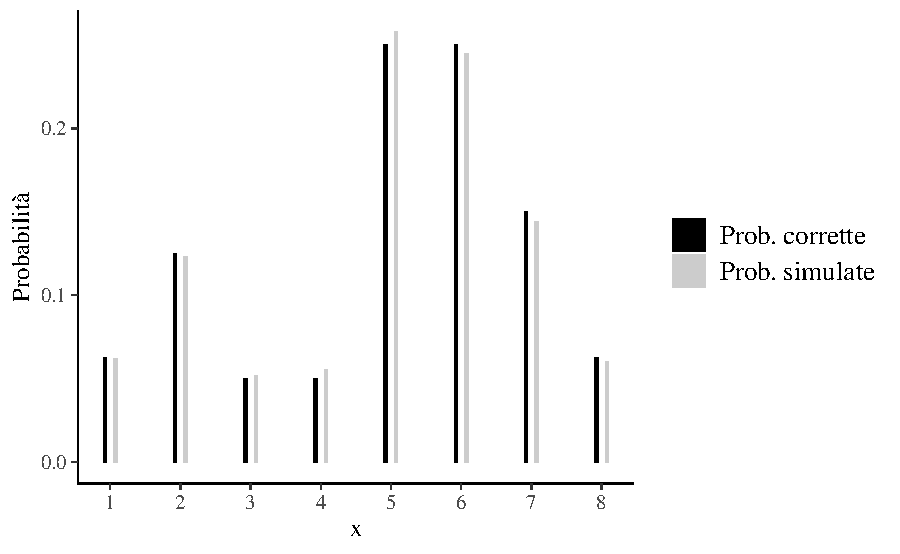
\includegraphics{ds4psy_files/figure-latex/metropolishistogramsim-1} 

}

\caption{L'istogramma confronta i valori prodotti dall'algoritmo di Metropolis con i valori corretti della distribuzione di massa di probabilità.}\label{fig:metropolishistogramsim}
\end{figure}

La figura \ref{fig:metropolishistogramsim} confronta l'istogramma dei valori simulati dalla passeggiata casuale con l'effettiva distribuzione di probabilità \texttt{pd}. Si noti la somiglianza tra le due distribuzioni.

\hypertarget{lalgoritmo-di-metropolis}{%
\subsection{L'algoritmo di Metropolis}\label{lalgoritmo-di-metropolis}}

Dopo avere introdotto l'algoritmo di Metropolis con l'esempio proposto da \citet{albert2019probability}, esaminiamo nuovamente tale algoritmo considerando un caso più generale. Ci poniamo ora il problema di usare l'algoritmo di Metropolis per per generare una catena di Markov irriducibile e aperiodica la cui distribuzione stazionaria corrisponde alla distribuzione a posteriori di interesse.\footnote{Una illustrazione visiva di come si svolge il processo di ``esplorazione'' dell'algoritmo di Metropolis è fornita in questo \href{https://elevanth.org/blog/2017/11/28/build-a-better-markov-chain/}{post}.} In termini generali, l'algoritmo di Metropolis include due fasi.

\begin{itemize}
\tightlist
\item
  \emph{Fase 1.} La selezione di un valore candidato \(\theta'\) del parametro mediante il campionamento da una distribuzione proposta.
\item
  \emph{Fase 2.} La decisione tra la possibilità di accettare il valore candidato \(\theta^{(m+1)} = \theta'\) o di mantenere il valore corrente \(\theta^{(m+1)} = \theta\) sulla base del seguente criterio:

  \begin{itemize}
  \tightlist
  \item
    se \(\mathcal{L}(\theta' \mid y)p(\theta') > \mathcal{L}(\theta \mid y)p(\theta)\) il valore candidato viene sempre accettato;
  \item
    altrimenti il valore candidato viene accettato solo in una certa proporzione di casi.
  \end{itemize}
\end{itemize}

In maggiori dettagli, l'algoritmo di Metropolis può essere descritto nel modo seguente.

\begin{enumerate}
\def\labelenumi{(\alph{enumi})}
\item
  Si inizia con un punto arbitrario \(\theta^{(1)}\); quindi il primo valore della catena di Markov \(\theta^{(1)}\) può corrispondere semplicemente ad un valore a caso tra i valori possibili del parametro.
\item
  Per ogni passo successivo della catena, \(m + 1\), si campiona un valore candidato \(\theta'\) da una distribuzione proposta: \(\theta' \sim \Pi(\theta)\). La distribuzione proposta può essere qualunque distribuzione, anche se, idealmente, è meglio che sia simile alla distribuzione a posteriori. In pratica, però, la distribuzione a posteriori è sconosciuta e quindi il valore \(\theta'\) viene campionato da una qualche distribuzione simmetrica centrata sul valore corrente \(\theta^{(m)}\) del parametro. Nell'esempio discusso qui di seguito, useremo la distribuzione gaussiana. Tale distribuzione sarà centrata sul valore corrente della catena e avrà una appropriata deviazione standard: \(\theta' \sim \mathcal{N}(\theta^{(m)}, \sigma)\). In pratica, questo significa che, se \(\sigma\) è piccola, il candidato \(\theta'\) avrà un valore simile al valore corrente \(\theta^{(m)}\).
\item
  Una volta generato il valore candidato \(\theta'\) si calcola il rapporto tra la densità della distribuzione a posteriori non normalizzata nel punto \(\theta'\) {[}ovvero, il prodotto tra la verosimiglianza \(\mathcal{L}(y \mid \theta')\) nel punto \(\theta'\) e la densità della distribuzione a priori nel punto \(\theta'\){]} e la densità della distribuzione a posteriori non normalizzata nel punto \(\theta^{(m)}\) {[}ovvero, il prodotto tra la verosimiglianza \(\mathcal{L}(y \mid \theta^{(m)})\) nel punto \(\theta^{(m)}\) e la densità della distribuzione a priori nel punto \(\theta^{(m)}\){]}:
\end{enumerate}

\begin{equation}
\alpha = \frac{p(y \mid \theta') p(\theta')}{p(y \mid \theta^{(m)}) p(\theta^{(m)})}.
\label{eq:ratio-metropolis}
\end{equation}

Si noti che, essendo un rapporto, la \eqref{eq:ratio-metropolis} cancella la costante di normalizzazione.

\begin{enumerate}
\def\labelenumi{(\alph{enumi})}
\setcounter{enumi}{3}
\item
  Il rapporto \(\alpha\) viene utilizzato per decidere se accettare il valore candidato \(\theta'\), oppure se campionare un diverso candidato. Possiamo pensare al rapporto \(\alpha\) come alla risposta alla seguente domanda: alla luce dei dati, è più plausibile il valore candidato del parametro o il valore corrente? Se \(\alpha\) è maggiore di 1 ciò significa che il valore candidato è più plausibile del valore corrente; in tali circostanze il valore candidato viene sempre accettato. Altrimenti, si decide di accettare il valore candidato con una probabilità minore di 1, ovvero non sempre, ma soltanto con una probabilità uguale ad \(\alpha\). Se \(\alpha\) è uguale a 0.10, ad esempio, questo significa che la credibilità a posteriori del valore candidato è 10 volte più piccola della credibilità a posteriori del valore corrente. Dunque, il valore candidato verrà accettato solo nel 10\% dei casi. Come conseguenza di questa strategia di scelta, l'algoritmo di Metropolis ottiene un campione casuale dalla distribuzione a posteriori, dato che la probabilità di accettare il valore candidato è proporzionale alla densità del candidato nella distribuzione a posteriori. Dal punto di vista algoritmico, la procedura descritta sopra viene implementata confrontando il rapporto \(\alpha\) con un valore casuale estratto da una distribuzione uniforme \(\mbox{Unif}(0, 1)\). Se \(\alpha > u \sim \mbox{Unif}(0, 1)\), allora il valore candidato \(\theta'\) viene accettato e la catena si muove in quella nuova posizione, ovvero \(\theta^{(m+1)} = \theta'\). Altrimenti \(\theta^{(m+1)} = \theta^{(m)}\) e si campiona un nuovo valore candidato \(\theta'\).
\item
  Il passaggio finale dell'algoritmo calcola l'\emph{accettanza} in una specifica esecuzione dell'algoritmo, ovvero la proporzione dei valori candidati \(\theta'\) che sono stati accettati come valori successivi nella sequenza.
\end{enumerate}

L'algoritmo di Metropolis prende come input il numero \(M\) di passi da simulare, la deviazione standard \(\sigma\) della distribuzione proposta e la densità a priori, e ritorna come output la sequenza \(\theta^{(1)}, \theta^{(2)}, \dots, \theta^{(M)}\). La chiave del successo dell'algoritmo di Metropolis è il numero di passi fino a che la catena approssima la stazionarietà. Tipicamente i primi da 1000 a 5000 elementi sono scartati. Dopo un certo periodo \(k\) (detto di \emph{burn-in}), la catena di Markov converge ad una variabile casuale che è distribuita secondo la distribuzione a posteriori. In altre parole, i campioni del vettore \(\left(\theta^{(k+1)}, \theta^{(k+2)}, \dots, \theta^{(M)}\right)\) diventano campioni di \(p(\theta \mid y)\).

\hypertarget{un-esempio-concreto-4}{%
\subsection{Un esempio concreto}\label{un-esempio-concreto-4}}

Consideriamo nuovamente i 30 pazienti esaminati da \citet{zetschefuture2019}. Di essi, 23 hanno manifestato aspettative distorte negativamente sul loro stato d'animo futuro. Utilizzando l'algoritmo di Metropolis, ci poniamo il problema di ottenere la stima a posteriori di \(\theta\) (probabilità di manifestare un'aspettativa distorta negativamente), dati 23 ``successi'' in 30 prove, e imponendo su \(\theta\) la stessa distribuzione a priori usata nel Capitolo \ref{chapter-distr-coniugate}, ovvero \(\mbox{Beta}(2, 10)\).\footnote{L'Appendice \ref{es-pratico-zetsche-funzioni} mostra come un'approssimazione della distribuzione a posteriori \(p(\theta \mid y)\) per questi dati possa essere ottenuta mediante il metodo basato su griglia.}

\hypertarget{funzioni}{%
\subsubsection{Funzioni}\label{funzioni}}

Per calcolare la funzione di verosimiglianza definiamo la funzione \texttt{likelihood()}

\begin{Shaded}
\begin{Highlighting}[]
\NormalTok{likelihood }\OtherTok{\textless{}{-}} \ControlFlowTok{function}\NormalTok{(param, }\AttributeTok{x =} \DecValTok{23}\NormalTok{, }\AttributeTok{N =} \DecValTok{30}\NormalTok{) \{}
  \FunctionTok{dbinom}\NormalTok{(x, N, param)}
\NormalTok{\}}
\end{Highlighting}
\end{Shaded}

che, avendo fissato i dati di \citet{zetschefuture2019}, ritorna l'ordinata della verosimiglianza binomiale per ciascun valore \texttt{param} in input.

La distribuzione a priori \(\mbox{Beta}(2, 10)\) è implementata nella funzione \texttt{prior()}:

\begin{Shaded}
\begin{Highlighting}[]
\NormalTok{prior }\OtherTok{\textless{}{-}} \ControlFlowTok{function}\NormalTok{(param, }\AttributeTok{alpha =} \DecValTok{2}\NormalTok{, }\AttributeTok{beta =} \DecValTok{10}\NormalTok{) \{}
  \FunctionTok{dbeta}\NormalTok{(param, alpha, beta) }
\NormalTok{\}}
\end{Highlighting}
\end{Shaded}

Questa funzione ritorna l'ordinata della distribuzione a priori che è stata definita, per ciascun valore \texttt{param} in input.

La funzione \texttt{posterior()} ritorna, per ciascun valore \texttt{param} in input, il prodotto della densità a priori e della verosimiglianza:

\begin{Shaded}
\begin{Highlighting}[]
\NormalTok{posterior }\OtherTok{\textless{}{-}} \ControlFlowTok{function}\NormalTok{(param) \{}
  \FunctionTok{likelihood}\NormalTok{(param) }\SpecialCharTok{*} \FunctionTok{prior}\NormalTok{(param)}
\NormalTok{\}}
\end{Highlighting}
\end{Shaded}

\hypertarget{implementazione}{%
\subsubsection{Implementazione}\label{implementazione}}

Per implementare l'algoritmo di Metropolis utilizzeremo una distribuzione proposta gaussiana. Il valore candidato sarà dunque un valore selezionato a caso da una gaussiana di parametri \(\mu\) uguale al valore corrente nella catena e \(\sigma = 0.9\). In questo esempio, la deviazione standard \(\sigma\) è stata scelta empiricamente in modo tale da ottenere una accettanza adeguata. L'accettanza ottimale èpari a circa 0.20/0.30 --- se l'accettanza è troppo grande, l'algoritmo esplora uno spazio troppo ristretto della distribuzione a posteriori.\footnote{L'accettanza dipende dalla distribuzione proposta: in generale, tanto più la distribuzione proposta è simile alla distribuzione target, tanto più alta diventa l'accettanza.}

\begin{Shaded}
\begin{Highlighting}[]
\NormalTok{proposal\_distribution }\OtherTok{\textless{}{-}} \ControlFlowTok{function}\NormalTok{(param) \{}
  \ControlFlowTok{while}\NormalTok{(}\DecValTok{1}\NormalTok{) \{}
\NormalTok{    res }\OtherTok{=} \FunctionTok{rnorm}\NormalTok{(}\DecValTok{1}\NormalTok{, }\AttributeTok{mean =}\NormalTok{ param, }\AttributeTok{sd =} \FloatTok{0.9}\NormalTok{)}
    \ControlFlowTok{if}\NormalTok{ (res }\SpecialCharTok{\textgreater{}} \DecValTok{0} \SpecialCharTok{\&}\NormalTok{ res }\SpecialCharTok{\textless{}} \DecValTok{1}\NormalTok{)}
      \ControlFlowTok{break}
\NormalTok{  \}}
\NormalTok{  res}
\NormalTok{\}}
\end{Highlighting}
\end{Shaded}

Nella presente implementazione del campionamento dalla distribuzione proposta è stato inserito un controllo che impone al valore candidato di essere incluso nell'intervallo {[}0, 1{]}, com'è necessario per il valore di una proporzione.\footnote{Si possono trovare implementazioni più eleganti dell'algoritmo di Metropolis di quella presentata qui. Il presente esercizio ha solo lo scopo di illustrare la logica soggiacente all'algoritmo di Metropolis; non ci poniamo qui il problema di trovare un'implementazione efficente dell'algoritmo.}

L'algoritmo di Metropolis viene implementato nella seguente funzione:

\begin{Shaded}
\begin{Highlighting}[]
\NormalTok{run\_metropolis\_MCMC }\OtherTok{\textless{}{-}} \ControlFlowTok{function}\NormalTok{(startvalue, iterations) \{}
\NormalTok{  chain }\OtherTok{\textless{}{-}} \FunctionTok{vector}\NormalTok{(}\AttributeTok{length =}\NormalTok{ iterations }\SpecialCharTok{+} \DecValTok{1}\NormalTok{)}
\NormalTok{  chain[}\DecValTok{1}\NormalTok{] }\OtherTok{\textless{}{-}}\NormalTok{ startvalue}
  \ControlFlowTok{for}\NormalTok{ (i }\ControlFlowTok{in} \DecValTok{1}\SpecialCharTok{:}\NormalTok{iterations) \{}
\NormalTok{    proposal }\OtherTok{\textless{}{-}} \FunctionTok{proposal\_distribution}\NormalTok{(chain[i])}
\NormalTok{    r }\OtherTok{\textless{}{-}} \FunctionTok{posterior}\NormalTok{(proposal) }\SpecialCharTok{/} \FunctionTok{posterior}\NormalTok{(chain[i])}
    \ControlFlowTok{if}\NormalTok{ (}\FunctionTok{runif}\NormalTok{(}\DecValTok{1}\NormalTok{) }\SpecialCharTok{\textless{}}\NormalTok{ r) \{}
\NormalTok{      chain[i }\SpecialCharTok{+} \DecValTok{1}\NormalTok{] }\OtherTok{\textless{}{-}}\NormalTok{ proposal}
\NormalTok{    \} }\ControlFlowTok{else}\NormalTok{ \{}
\NormalTok{      chain[i }\SpecialCharTok{+} \DecValTok{1}\NormalTok{] }\OtherTok{\textless{}{-}}\NormalTok{ chain[i]}
\NormalTok{    \}}
\NormalTok{  \}}
\NormalTok{  chain}
\NormalTok{\}}
\end{Highlighting}
\end{Shaded}

Avendo definito le funzioni precedenti, possiamo ora generare una catena di valori \(\theta\):

\begin{Shaded}
\begin{Highlighting}[]
\FunctionTok{set.seed}\NormalTok{(}\DecValTok{84735}\NormalTok{)}
\NormalTok{startvalue }\OtherTok{\textless{}{-}} \FunctionTok{runif}\NormalTok{(}\DecValTok{1}\NormalTok{, }\DecValTok{0}\NormalTok{, }\DecValTok{1}\NormalTok{)}
\NormalTok{niter }\OtherTok{\textless{}{-}} \FloatTok{1e4}
\NormalTok{chain }\OtherTok{\textless{}{-}} \FunctionTok{run\_metropolis\_MCMC}\NormalTok{(startvalue, niter)}
\end{Highlighting}
\end{Shaded}

Mediante le istruzioni precedenti otteniamo una catena di Markov costituita da 10,001 valori. Escludiamo i primi 5,000 valori considerati come burn-in. Ci restano dunque con 5,001 valori che verranno considerati come un campione casuale estratto dalla distribuzione a posteriori \(p(\theta \mid y)\).

L'accettanza è pari a

\begin{Shaded}
\begin{Highlighting}[]
\NormalTok{burnIn }\OtherTok{\textless{}{-}}\NormalTok{ niter }\SpecialCharTok{/} \DecValTok{2}
\NormalTok{acceptance }\OtherTok{\textless{}{-}} \DecValTok{1} \SpecialCharTok{{-}} \FunctionTok{mean}\NormalTok{(}\FunctionTok{duplicated}\NormalTok{(chain[}\SpecialCharTok{{-}}\NormalTok{(}\DecValTok{1}\SpecialCharTok{:}\NormalTok{burnIn)]))}
\NormalTok{acceptance}
\CommentTok{\#\textgreater{} [1] 0.2585}
\end{Highlighting}
\end{Shaded}

\noindent il che conferma la bontà della deviazione standard (\(\sigma\) = 0.9) scelta per la distribuzione proposta.

A questo punto è facile ottenere una stima a posteriori del parametro \(\theta\). Per esempio, la stima della media a posteriori è:

\begin{Shaded}
\begin{Highlighting}[]
\FunctionTok{mean}\NormalTok{(chain[}\SpecialCharTok{{-}}\NormalTok{(}\DecValTok{1}\SpecialCharTok{:}\NormalTok{burnIn)])}
\CommentTok{\#\textgreater{} [1] 0.5957}
\end{Highlighting}
\end{Shaded}

Una figura che mostra l'approssimazione di \(p(\theta \mid y)\) ottenuta con l'algoritmo di Metropolis, insieme ad un \emph{trace plot} dei valori della catena di Markov, viene prodotta usando le seguenti istruzioni:

\begin{Shaded}
\begin{Highlighting}[]
\NormalTok{p1 }\OtherTok{\textless{}{-}} \FunctionTok{tibble}\NormalTok{(}
  \AttributeTok{x =}\NormalTok{ chain[}\SpecialCharTok{{-}}\NormalTok{(}\DecValTok{1}\SpecialCharTok{:}\NormalTok{burnIn)]}
\NormalTok{) }\SpecialCharTok{\%\textgreater{}\%}
  \FunctionTok{ggplot}\NormalTok{(}\FunctionTok{aes}\NormalTok{(x)) }\SpecialCharTok{+}
  \FunctionTok{geom\_histogram}\NormalTok{() }\SpecialCharTok{+}
  \FunctionTok{labs}\NormalTok{(}
    \AttributeTok{x =} \FunctionTok{expression}\NormalTok{(theta),}
    \AttributeTok{y =} \StringTok{"Frequenza"}\NormalTok{,}
    \AttributeTok{title =} \StringTok{"Distribuzione a posteriori"}
\NormalTok{  ) }\SpecialCharTok{+}
  \FunctionTok{geom\_vline}\NormalTok{(}
    \AttributeTok{xintercept =} \FunctionTok{mean}\NormalTok{(chain[}\SpecialCharTok{{-}}\NormalTok{(}\DecValTok{1}\SpecialCharTok{:}\NormalTok{burnIn)])}
\NormalTok{  ) }\SpecialCharTok{+}
  \FunctionTok{xlim}\NormalTok{(}\FunctionTok{c}\NormalTok{(}\FloatTok{0.3}\NormalTok{, }\FloatTok{0.85}\NormalTok{)) }\SpecialCharTok{+}
  \FunctionTok{coord\_flip}\NormalTok{()}

\NormalTok{p2 }\OtherTok{\textless{}{-}} \FunctionTok{tibble}\NormalTok{(}
  \AttributeTok{x =} \DecValTok{1}\SpecialCharTok{:}\FunctionTok{length}\NormalTok{(chain[}\SpecialCharTok{{-}}\NormalTok{(}\DecValTok{1}\SpecialCharTok{:}\NormalTok{burnIn)]),}
  \AttributeTok{y =}\NormalTok{ chain[}\SpecialCharTok{{-}}\NormalTok{(}\DecValTok{1}\SpecialCharTok{:}\NormalTok{burnIn)]}
\NormalTok{) }\SpecialCharTok{\%\textgreater{}\%}
  \FunctionTok{ggplot}\NormalTok{(}\FunctionTok{aes}\NormalTok{(x, y)) }\SpecialCharTok{+}
  \FunctionTok{geom\_line}\NormalTok{() }\SpecialCharTok{+}
  \FunctionTok{labs}\NormalTok{(}
    \AttributeTok{x =} \StringTok{"Numero di passi"}\NormalTok{,}
    \AttributeTok{y =} \FunctionTok{expression}\NormalTok{(theta),}
    \AttributeTok{title =} \StringTok{"Valori della catena"}
\NormalTok{  ) }\SpecialCharTok{+}
  \FunctionTok{geom\_hline}\NormalTok{(}
    \AttributeTok{yintercept =} \FunctionTok{mean}\NormalTok{(chain[}\SpecialCharTok{{-}}\NormalTok{(}\DecValTok{1}\SpecialCharTok{:}\NormalTok{burnIn)]),}
    \AttributeTok{colour =} \StringTok{"gray"}
\NormalTok{  ) }\SpecialCharTok{+}
  \FunctionTok{ylim}\NormalTok{(}\FunctionTok{c}\NormalTok{(}\FloatTok{0.3}\NormalTok{, }\FloatTok{0.85}\NormalTok{)) }

\NormalTok{p1 }\SpecialCharTok{+}\NormalTok{ p2}
\end{Highlighting}
\end{Shaded}

\begin{figure}[h]

{\centering 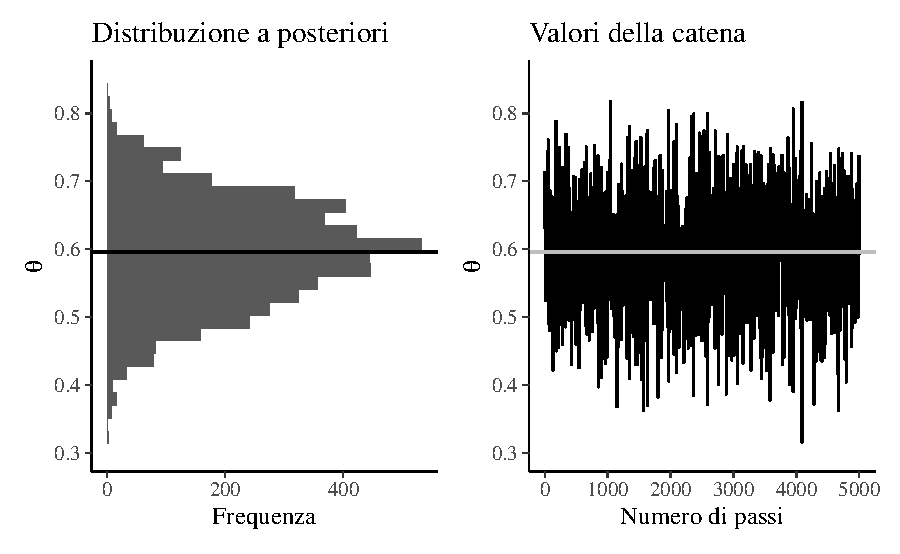
\includegraphics{ds4psy_files/figure-latex/sim-markov-chain-zetsche-1} 

}

\caption{Sinistra. Stima della distribuzione a posteriori della probabilità di una aspettativa futura distorta negativamente per i dati di Zetsche et al. (2019). Destra. Trace plot dei valori della catena di Markov escludendo il periodo di burn-in.}\label{fig:sim-markov-chain-zetsche}
\end{figure}

\hypertarget{input}{%
\subsection{Input}\label{input}}

Negli esempi discussi in questo Capitolo abbiamo illustrato l'esecuzione di una singola catena in cui si parte un unico valore iniziale e si raccolgono i valori simulati da molte iterazioni. È possibile però che i valori di una catena siano influenzati dalla scelta del valore iniziale. Quindi una raccomandazione generale è di eseguire l'algoritmo di Metropolis più volte utilizzando diversi valori di partenza. In questo caso, si avranno più catene di Markov. Confrontando le proprietà delle diverse catene si esplora la sensibilità dell'inferenza alla scelta del valore di partenza. I software MCMC consentono sempre all'utente di specificare diversi valori di partenza e di generare molteplici catene di Markov.

\hypertarget{stazionarietuxe0}{%
\subsection{Stazionarietà}\label{stazionarietuxe0}}

Un punto importante da verificare è se il campionatore ha raggiunto la sua distribuzione stazionaria. La convergenza di una catena di Markov alla distribuzione stazionaria viene detta ``mixing''.

\hypertarget{approx-post-autocor}{%
\subsubsection{Autocorrelazione}\label{approx-post-autocor}}

Informazioni sul ``mixing'' della catena di Markov sono fornite dall'autocorrelazione. L'autocorrelazione misura la correlazione tra i valori successivi di una catena di Markov. Il valore \(m\)-esimo della serie ordinata viene confrontato con un altro valore ritardato di una quantità \(k\) (dove \(k\) è l'entità del ritardo) per verificare quanto si correli al variare di \(k\). L'autocorrelazione di ordine 1 (\emph{lag 1}) misura la correlazione tra valori successivi della catena di Markow (cioè, la correlazione tra \(\theta^{(m)}\) e \(\theta^{(m-1)}\)); l'autocorrelazione di ordine 2 (\emph{lag 2}) misura la correlazione tra valori della catena di Markow separati da due ``passi'' (cioè, la correlazione tra \(\theta^{(m)}\) e \(\theta^{(m-2)}\)); e così via.

L'autocorrelazione di ordine \(k\) è data da \(\rho_k\) e può essere stimata come:

\begin{align}
\rho_k &= \frac{\Cov(\theta_m, \theta_{m+k})}{\Var(\theta_m)}\notag\\
&= \frac{\sum_{m=1}^{n-k}(\theta_m - \bar{\theta})(\theta_{m-k} - \bar{\theta})}{\sum_{m=1}^{n-k}(\theta_m - \bar{\theta})^2} \qquad\text{con }\quad \bar{\theta} = \frac{1}{n}\sum_{m=1}^{n}\theta_m.
\label{eq:autocor}
\end{align}

Per fare un esempio pratico, simuliamo dei dati autocorrelati con la funzione R \texttt{colorednoise::colored\_noise()}:

\begin{Shaded}
\begin{Highlighting}[]
\FunctionTok{suppressPackageStartupMessages}\NormalTok{(}\FunctionTok{library}\NormalTok{(}\StringTok{"colorednoise"}\NormalTok{))}
\FunctionTok{set.seed}\NormalTok{(}\DecValTok{34783859}\NormalTok{)}
\NormalTok{rednoise }\OtherTok{\textless{}{-}} \FunctionTok{colored\_noise}\NormalTok{(}
  \AttributeTok{timesteps =} \DecValTok{30}\NormalTok{, }\AttributeTok{mean =} \FloatTok{0.5}\NormalTok{, }\AttributeTok{sd =} \FloatTok{0.05}\NormalTok{, }\AttributeTok{phi =} \FloatTok{0.3}
\NormalTok{)}
\end{Highlighting}
\end{Shaded}

L'autocorrelazione di ordine 1 è semplicemente la correlazione tra ciascun elemento e quello successivo nella sequenza. Nell'esempio, il vettore \texttt{rednoise} è una sequenza temporale di 30 elementi. Il vettore \texttt{rednoise{[}-length(rednoise){]}} include gli elementi con gli indici da 1 a 29 nella sequenza originaria, mentre il vettore \texttt{rednoise{[}-1{]}} include gli elementi 2:30. Gli elementi delle coppie ordinate dei due vettori avranno dunque gli indici \((1, 2), (2, 3), \dots (29, 30)\) degli elementi della sequenza originaria. La correlazione di Pearson tra i vettori \texttt{rednoise{[}-length(rednoise){]}} e \texttt{rednoise{[}-1{]}} corrisponde all'autocorrelazione di ordine 1 della serie temporale.

\begin{Shaded}
\begin{Highlighting}[]
\FunctionTok{cor}\NormalTok{(rednoise[}\SpecialCharTok{{-}}\FunctionTok{length}\NormalTok{(rednoise)], rednoise[}\SpecialCharTok{{-}}\DecValTok{1}\NormalTok{])}
\CommentTok{\#\textgreater{} [1] 0.3967}
\end{Highlighting}
\end{Shaded}

Il Correlogramma è uno strumento grafico usato per la valutazione della tendenza di una catena di Markov nel tempo. Il correlogramma si costruisce a partire dall'autocorrelazione \(\rho_k\) di una catena di Markov in funzione del ritardo (\emph{lag}) \(k\) con cui l'autocorrelazione è calcolata: nel grafico ogni barretta verticale riporta il valore dell'autocorrelazione (sull'asse delle ordinate) in funzione del ritardo (sull'asse delle ascisse). In \(\R\), il correlogramma può essere prodotto con una chiamata a \texttt{acf()}:

\begin{Shaded}
\begin{Highlighting}[]
\FunctionTok{acf}\NormalTok{(rednoise)}
\end{Highlighting}
\end{Shaded}

\begin{center}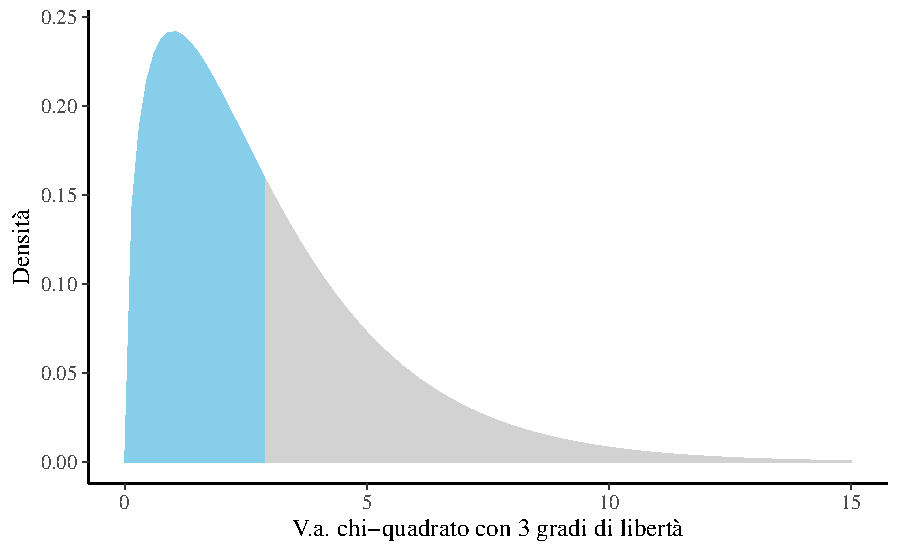
\includegraphics{ds4psy_files/figure-latex/unnamed-chunk-56-1} \end{center}

Nel correlogramma precedente vediamo che l'autocorrelazione di ordine 1 è circa pari a 0.4 e diminuisce per lag maggiori; per lag di 4, l'autocorrelazione diventa negativa e aumenta progressivamente fino ad un lag di 8; eccetera.

In situazioni ottimali l'autocorrelazione diminuisce rapidamente ed è effettivamente pari a 0 per piccoli lag. Ciò indica che i valori della catena di Markov che si trovano a più di soli pochi passi di distanza gli uni dagli altri non risultano associati tra loro, il che fornisce una conferma del ``mixing'' della catena di Markov, ossia della convergenza alla distribuzione stazionaria. Nelle analisi bayesiane, una delle strategie che consentono di ridurre l'autocorrelazione è quella di assottigliare l'output immagazzinando solo ogni \(m\)-esimo punto dopo il periodo di burn-in. Una tale strategia va sotto il nome di \emph{thinning}.

\hypertarget{test-di-convergenza}{%
\subsection{Test di convergenza}\label{test-di-convergenza}}

Un test di convergenza può essere svolto in maniera grafica mediante le tracce delle serie temporali (\emph{trace plot}), cioè il grafico dei valori simulati rispetto al numero di iterazioni. Se la catena è in uno stato stazionario le tracce mostrano assenza di periodicità nel tempo e ampiezza costante, senza tendenze visibili o andamenti degni di nota. Un esempio di \emph{trace plot} è fornito nella figura \ref{fig:sim-markov-chain-zetsche} (destra).

Ci sono inoltre alcuni test che permettono di verificare la stazionarietà del campionatore dopo un dato punto. Uno è il test di Geweke che suddivide il campione, dopo aver rimosso un periodo di burn in, in due parti. Se la catena è in uno stato stazionario, le medie dei due campioni dovrebbero essere uguali. Un test modificato, chiamato Geweke z-score, utilizza un test \(z\) per confrontare i due subcampioni ed il risultante test statistico, se ad esempio è più alto di 2, indica che la media della serie sta ancora muovendosi da un punto ad un altro e quindi è necessario un periodo di burn-in più lungo.

\hypertarget{commenti-e-considerazioni-finali-3}{%
\section*{Commenti e considerazioni finali}\label{commenti-e-considerazioni-finali-3}}


In generale, la distribuzione a posteriori dei parametri di un modello statistico non può essere determinata per via analitica. Tale problema viene invece affrontato facendo ricorso ad una classe di algoritmi per il campionamento da distribuzioni di probabilità che sono estremamente onerosi dal punto di vista computazionale e che possono essere utilizzati nelle applicazioni pratiche solo grazie alla potenza di calcolo dei moderni computer. Lo sviluppo di software che rendono sempre più semplice l'uso dei metodi MCMC, insieme all'incremento della potenza di calcolo dei computer, ha contribuito a rendere sempre più popolare il metodo dell'inferenza bayesiana che, in questo modo, può essere estesa a problemi di qualunque grado di complessità.

\mainmatter

\hypertarget{part-appendici}{%
\part{Appendici}\label{part-appendici}}

\hypertarget{appendix-appendici}{%
\appendix \addcontentsline{toc}{chapter}{\appendixname}}


\hypertarget{appendix:quadratic-approx}{%
\chapter{Approssimazione quadratica}\label{appendix:quadratic-approx}}

L'approssimazione quadratica è un metodo analitico approssimato che può essere usato per superare il problema della ``maledizione della dimensionalità''. La motivazione di tale metodo è la seguente. Sappiamo che, in generale, la regione della distribuzione a posteriori che si trova in prossimità del suo massimo può essere ben approssimata dalla forma di una distribuzione gaussiana.\footnote{Descrivere la distribuzione a posteriori mediante la distribuzione gaussiana significa utilizzare un'approssimazione che viene, appunto, chiamata ``quadratica''. Tale approssimazione si dice quadratica perché il logaritmo di una distribuzione gaussiana forma una parabola e la parabola è una funzione quadratica -- dunque, mediante questa approssimazione descriviamo il logaritmo della distribuzione a posteriori mediante una parabola.}

L'approssimazione quadratica si pone due obiettivi.

\begin{enumerate}
\def\labelenumi{\arabic{enumi}.}
\tightlist
\item
  Trovare la moda della distribuzione a posteriori. Ci sono varie procedure di ottimizzazione, implementate in \(\R\), in grado di trovare il massimo di una distribuzione.
\item
  Stimare la curvatura della distribuzione in prossimità della moda. Una stima della curvatura è sufficiente per trovare un'approssimazione quadratica dell'intera distribuzione. In alcuni casi, questi calcoli possono essere fatti seguendo una procedura analitica, ma solitamente vengono usate delle tecniche numeriche.
\end{enumerate}

Per fare un esempio concreto, consideriamo nuovamente i dati di \citet{zetschefuture2019} (ovvero, 23 ``successi'' in 30 prove Bernoulliane). Supponiamo di usare una \(\mbox{Beta}(2, 10)\) quale distribuzione a priori per il parametro sconosciuto \(\theta\) (probabilità che l'aspettativa dell'umore futuro sia distorta negativamente). Una descrizione della distribuzione a posteriori ottenuta mediante l'approssimazione quadratica si ottiene utilizzando la funzione \texttt{quap()} del pacchetto \texttt{rethinking}:\footnote{Il pacchetto \texttt{rethinking} è stato creato da \citet{McElreath_rethinking} per accompagnare il suo testo \emph{Statistical Rethinking}\(^2\). Per l'installazione si veda \url{https://github.com/rmcelreath/rethinking}.} Dopo avere specificato il modello utilizzando la sintassi appropriata

\begin{Shaded}
\begin{Highlighting}[]
\FunctionTok{suppressPackageStartupMessages}\NormalTok{(}\FunctionTok{library}\NormalTok{(}\StringTok{"rethinking"}\NormalTok{))}

\NormalTok{mod }\OtherTok{\textless{}{-}} \FunctionTok{quap}\NormalTok{(}
  \FunctionTok{alist}\NormalTok{(}
\NormalTok{  N }\SpecialCharTok{\textasciitilde{}} \FunctionTok{dbinom}\NormalTok{(N }\SpecialCharTok{+}\NormalTok{ P, p),}
\NormalTok{  p }\SpecialCharTok{\textasciitilde{}} \FunctionTok{dbeta}\NormalTok{(}\DecValTok{2}\NormalTok{, }\DecValTok{10}\NormalTok{) }
\NormalTok{  ),}
  \AttributeTok{data =} \FunctionTok{list}\NormalTok{(}\AttributeTok{N =} \DecValTok{23}\NormalTok{, }\AttributeTok{P =} \DecValTok{7}\NormalTok{)}
\NormalTok{)}
\end{Highlighting}
\end{Shaded}

un sommario dell'approssimazione quadratica si ottiene con la funzione \texttt{precis()}:

\begin{Shaded}
\begin{Highlighting}[]
\FunctionTok{precis}\NormalTok{(mod, }\AttributeTok{prob =} \FloatTok{0.95}\NormalTok{)}
\CommentTok{\#\textgreater{}   mean      sd   2.5\%  97.5\%}
\CommentTok{\#\textgreater{} p  0.6 0.07746 0.4482 0.7518}
\end{Highlighting}
\end{Shaded}

La figura seguente fornisce un confronto tra la corretta distribuzione a posteriori (linea continua) e l'approssimazione quadratica (linea trateggiata).

\begin{Shaded}
\begin{Highlighting}[]
\NormalTok{N }\OtherTok{\textless{}{-}} \DecValTok{23}
\NormalTok{P }\OtherTok{\textless{}{-}} \DecValTok{7}
\NormalTok{a }\OtherTok{\textless{}{-}}\NormalTok{ N }\SpecialCharTok{+} \DecValTok{2}
\NormalTok{b }\OtherTok{\textless{}{-}}\NormalTok{ P }\SpecialCharTok{+} \DecValTok{10}
\FunctionTok{curve}\NormalTok{(}\FunctionTok{dbeta}\NormalTok{(x, a, b), }\AttributeTok{from=}\DecValTok{0}\NormalTok{, }\AttributeTok{to=}\DecValTok{1}\NormalTok{, }\AttributeTok{ylab=}\StringTok{"Densità"}\NormalTok{)}
\CommentTok{\# approssimazione quadratica}
\FunctionTok{curve}\NormalTok{(}
  \FunctionTok{dnorm}\NormalTok{(x, a}\SpecialCharTok{/}\NormalTok{(a}\SpecialCharTok{+}\NormalTok{b), }\FunctionTok{sqrt}\NormalTok{((a}\SpecialCharTok{*}\NormalTok{b)}\SpecialCharTok{/}\NormalTok{((a}\SpecialCharTok{+}\NormalTok{b)}\SpecialCharTok{\^{}}\DecValTok{2}\SpecialCharTok{*}\NormalTok{(a}\SpecialCharTok{+}\NormalTok{b}\SpecialCharTok{+}\DecValTok{1}\NormalTok{)))),}
  \AttributeTok{lty =} \DecValTok{2}\NormalTok{,}
  \AttributeTok{add =} \ConstantTok{TRUE}
\NormalTok{)}
\end{Highlighting}
\end{Shaded}

\begin{center}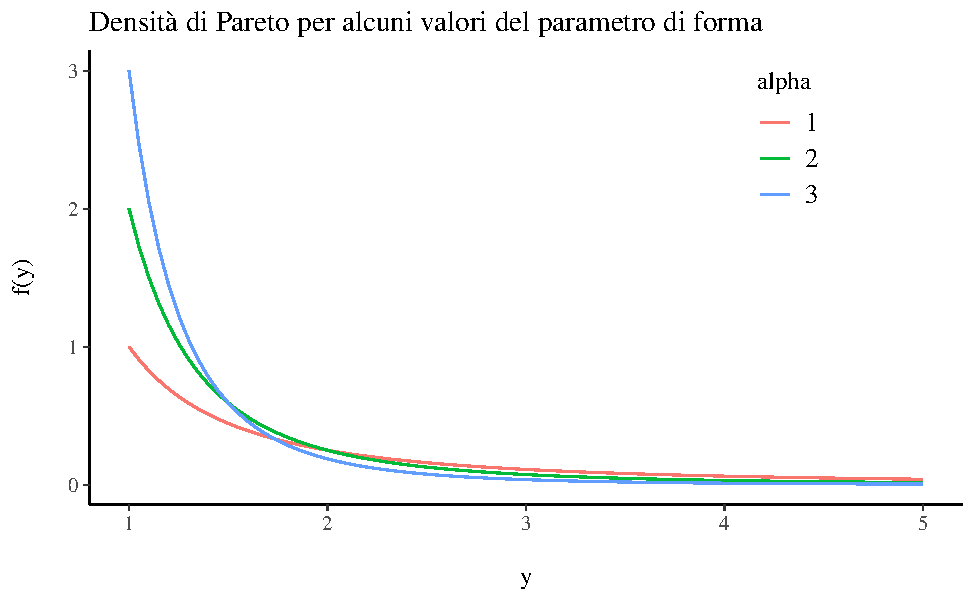
\includegraphics{ds4psy_files/figure-latex/unnamed-chunk-60-1} \end{center}

Il grafico precedente mostra che, nel caso dell'esempio, l'approssimazione quadratica fornisce un risultato soddisfacente. Tale risultato è quasi identico a quello che può essere trovato con il metodo \emph{grid-based}, con il vantaggio aggiuntivo che abbiamo accesso ad una serie di funzioni \(\R\) in grado di svolgere i calcoli per noi. In realtà, però, l'approssimazione quadratica è poco usata perché, per problemi complessi, è più conveniente fare ricorso ai metodi MCMC.

  \bibliography{refs.bib,book.bib,packages.bib}

\printindex

\end{document}
